\documentclass[
	12pt, %Schriftgröße
	a4paper, %Papierformat
	oneside, %einseitiger Druck, für zweiseitigen Druck weglassen
%	openany, %neue Kapitel dürfen auch auf linker Seite beginnen (beidseitiger Druck), sonst openright (default)
	chapterprefix, %Kapitelüberschriften zu Beginn eines Kapitels anzeigen
	listof=totoc, %Verzeichnisse (Abbildungen/Tabellen) im Inhaltsverzeichnis aufführen
%	draft, %Entwurfsmodus: lässt Links und Abbildungen weg, zeigt übervolle Zeilen an, wird schneller gesetzt
]{scrbook}

\newcommand*{\universitaet}[1]{\def\universitaet{#1}}
\newcommand*{\fach}[1]{\def\fach{#1}}
\newcommand*{\arbeitsart}[1]{\def\arbeitsart{#1}}
\newcommand*{\titel}[1]{\def\titel{#1}}
\newcommand*{\autor}[1]{\def\autor{#1}}
\newcommand*{\gutachter}[1]{\def\gutachter{#1}}
\newcommand*{\zweitgutachter}[1]{\def\zweitgutachter{#1}}
\newcommand*{\abteilung}[1]{\def\abteilung{#1}}
\newcommand*{\department}[1]{\def\department{#1}}
\newcommand*{\ort}[1]{\def\ort{#1}}
\newcommand*{\datum}[1]{\def\datum{#1}}

%---------------------------------
%---Sprache, Schrift & Encoding---
%---------------------------------

\usepackage[ngerman]{babel} %neue deutsche Rechtschreibung
\usepackage[utf8]{inputenc} %alternativ: ansinew (windows), latin1, latin9 (Linux/UNIX/Mac)

%\usepackage[T1]{fontenc} %einkommentieren, wenn Buchstaben/Schriftbild schief aussehen!
%\usepackage{lmodern} %andere Schrift, sieht evtl. besser aus

%------------
%---Layout---
%------------

\usepackage[
	left=3cm, %linker Seitenrand
	right=3cm, %rechter Seitenrand
	top=2.5cm, %oberer Seitenrand
	bottom=2.5cm, %unterer Seitenrand
]{geometry}
\usepackage[onehalfspacing]{setspace} %1,5-facher Zeilenabstand

%\usepackage{indentfirst} %rückt auch den ersten Absatz eines (Unter)abschnitts ein, so wie alle anderen Absätze auch

\usepackage[
	headsepline, %Kopfzeile durch Querlinie abheben
%	footsepline, %Fußzeile durch Querlinie abheben
	draft=false, %Kopf-/Fußzeile auch im draft-Modus (siehe documentclass) anzeigen
]{scrlayer-scrpage}
\clearpairofpagestyles
\ihead[]{\headmark} %Kapitel-/Abschnittsname innen in der Kopfzeile, außer zu Beginn neuer Kapitel
%\chead[]{}
\ohead*[]{\pagemark} %Seitenzahl außen in der Kopfzeile, außer zu Beginn neuer Kapitel
%\ifoot[]{}
%\cfoot[]{}
\ofoot*[\pagemark]{} %Seitenzahl außen in die Fußzeile, aber nur zu Beginn neuer Kapitel

\renewcommand*\chapterformat{\chapapp~\thechapter} %Kapitelüberschriften in der Form Kapitel~<Nummer>, siehe dazu chapterprefix in der documentclass

%-----------
%---Mathe---
%-----------

\usepackage{amsmath}
\usepackage{amsfonts}
\usepackage{amssymb}

%---------------
%---Sonstiges---
%---------------

\usepackage[sort&compress]{natbib} %ermöglicht die Verwendung von \citet{} und \citep{}
\bibliographystyle{dinat} %Zitierstil: andere auch möglich, z.B. alphadin, plain, ...

\usepackage{caption}
\usepackage{subcaption}
\usepackage{graphicx}
\usepackage{color}
\usepackage{transparent}
\usepackage{enumerate}
\usepackage{longtable}
\usepackage{wrapfig}
\usepackage{listings}
\usepackage{float}
%\usepackage[inkscape={C:/Program Files/Inkscape/bin/inkscape -z -C}]{svg}
\restylefloat{figure}
\graphicspath{{./Abbildungen/}, {./Abbildungen/Implementierung/}}

\DeclareFixedFont{\ttb}{T1}{txtt}{bx}{n}{10} % for bold
\DeclareFixedFont{\ttm}{T1}{txtt}{m}{n}{10}  % for normal

\definecolor{deepblue}{rgb}{0,0,0.5}
\definecolor{deepred}{rgb}{0.8,0,0}
\definecolor{deepgreen}{rgb}{0,0.5,0}
\definecolor{grey1}{rgb}{0.5,0.5,0.5}


% Python style for highlighting
\newcommand\pythonstyle{\lstset{
		language=Python,
		basicstyle=\small\ttm,
		otherkeywords={self},             % Add keywords here
		keywordstyle=\small\ttb\color{deepblue},
		emph={},          % Custom highlighting
		emphstyle=\small\color{deepred},    % Custom highlighting style
		stringstyle=\small\color{deepgreen},
		commentstyle=\small\color{grey1}\ttm,
		frame=tb,                         % Any extra options here
		showstringspaces=false,            % 
		breaklines=true,
		tabsize=2
}}
% Python environment
\lstnewenvironment{python}[1][] {
	\pythonstyle
	\lstset{#1}
}{}

% Python for external files
\newcommand\pythonexternal[2][]{{
		\pythonstyle
		\lstinputlisting[#1]{#2}}}

% Python for inline
\newcommand\pythoninline[1]{{\pythonstyle\lstinline!#1!}}

\usepackage[
	textsize=tiny, %kleinere Schrift als die default-Größe in den Notizen, damit mehr reinpasst
]{todonotes} %Notizen im Text mit

%------------------
%---Links & URLs---
%------------------

%hyperref möglichst als letztes package laden (es gibt aber Ausnahmen)!

\usepackage[
	urlcolor=black, %Textfarbe von Links schwarz statt blau (default)
]{hyperref} %für Referenzen, Verweise, Links, ...



%-----------------------------
%---Variablen zum ausfüllen---
%-----------------------------

\universitaet{Carl von Ossietzky Universität Oldenburg}
\fach{Wirtschaftsinformatik} %Informatik, ...
\arbeitsart{Bachelorarbeit} %Masterarbeit, Diplomarbeit, ...
\titel{Vergleich von verschiedenen Deep Reinforcement Learning Agenten am Beispiel des Videospiels Snake}
\autor{Lorenz Mumm}
\gutachter{Apl. Prof. Dr. Jürgen Sauer}
\zweitgutachter{M. Sc. Julius Möller}
\abteilung{Abteilung Systemanalyse und -optimierung}
\department{Department für Informatik}
\ort{Oldenburg}
\datum{\today} %Tag der Abgabe BEIM PRÜFUNGSAMT

%----------------
%---Titelseite---
%----------------
\begin{document}
\frontmatter %römische Seitennummerierung für den Anfang



\makeatletter
\begin{titlepage}
\centering
\begin{figure}[htb]
  \centering
  \begin{subfigure}{0.5\textwidth}
    \centering
    \includegraphics[scale=1.8]{Abbildungen/uni_ol_logo.png}
    \end{subfigure}%
    \begin{subfigure}{0.5\textwidth}
      \centering
      \includegraphics[scale=0.35]{Abbildungen/abteilungslogo.jpg}
    \end{subfigure}
\end{figure}

{\scshape\Large\universitaet\par}
\vspace{1cm}
{\scshape\normalsize\fach\par}
{\scshape\normalsize\arbeitsart\par}

\vfill

\hrule
\vspace{1cm}
{\LARGE\bfseries\titel\par}
\vspace{1cm}
\hrule

\vfill

\begin{minipage}[t]{0.4\textwidth}
  \begin{flushleft}
    {\normalsize\itshape Autor:\par}
    {\normalsize\autor}
  \end{flushleft}
\end{minipage}%
\begin{minipage}[t]{0.4\textwidth}
  \begin{flushright}
    {\normalsize\itshape Erstgutachter:\par}
    {\normalsize\gutachter}
  \end{flushright}
  \begin{flushright}
    {\normalsize\itshape Zweitgutachter:\par}
    {\normalsize\zweitgutachter}
  \end{flushright} 
\end{minipage}

\vfill

{\normalsize\abteilung\par}
{\normalsize\department\par}
\vspace{1cm}
{\normalsize\ort{}, \datum\par}
\end{titlepage}
\makeatother

%---------------
%---Abstracts---
%---------------

%einkommentieren, falls benötigt
%\input{Sonstiges/Abstract_deutsch.tex}
%\input{Sonstiges/Abstract_englisch.tex}

%-------------------
%---Verzeichnisse---
%-------------------

\tableofcontents %Inhaltsverzeichnis erzeugen
\listoffigures %Abbildungsverzeichnis erzeugen
\listoftables %Tabellenverzeichnis erzeugen

\chapter{Abkürzungsverzeichnis}
\begin{acronym}
	\acro{KI}[KI]{Künstliche Intelligenz}
	\acro{RL}[RL]{Reinforcement Learning}
	\acro{DQN}[DQN]{Deep Q-Network}
	\acro{DQL}[DQL]{Deep Q-Learning}
	\acro{DDQN}[DDQN]{Double Deep Q-Network}
	\acro{PPO}[PPO]{Proximal Policy Optimization}
	\acro{SAC}[SAC]{Soft Actor Critic}
	\acro{A2C}[A2C]{Advantage Actor Critic}
	\acro{Env}[Env]{Environment}
	\acro{Obs}[Obs]{Observation}
	\acro{AV}[AV]{around\_view}
	\acro{SO}[SO]{scalar\_obs}
\end{acronym}
  %auskommentieren, falls nicht benötigt

%---------------
%---Hauptteil---
%---------------

\mainmatter %arabische Seitennummerierung und nummerierte Kapitel ab dem Hauptteil

%die Kapitel der Arbeit in einzelnen Dateien anlegen und mit \input{} importieren
\chapter{Einleitung}\label{chap:Einleitung}
In dieser Ausarbeitung wird das Generische Maskulinum verwendet. Dieses soll niemanden beleidigen und oder diskriminieren.\\
\\Das Machine Learning ist weltweit auf dem Vormarsch und große Unternehmen investieren riesige Beträge, um mit KI basierten Lösungen größere Effizienz zu erreichen. Auch der Bereich des Reinforcement Learning gerät dabei immer mehr in das Blickfeld der Weltöffentlichkeit. Besonders im Gaming Bereich hat das Reinforcement Learning schon beeindruckende Resultate erbringen können, wie z.B. die KI AlphaGO, welche den amtierenden Weltmeister Lee Sedol im Spiel GO besiegt hat \citep{UAV}. In Anlehnung an die vielen neuen Reinforcement Learning Möglichkeiten, welche in der letzten Zeit entwickelt wurden und vor dem Hintergrund der immer größer werdenden Beliebtheit von KI basierten Lösungsstrategien, soll es in dieser Bachelorarbeit darum gehen, einzelnen Reinforcement Learning Agenten, mittels statistischer Methoden, genauer zu untersuchen und den optimalen Agenten für ein entsprechendes Problem zu bestimmen.

\section{Motivation} \label{sec:Einleitung_Motivation}
In den letzten Jahren erregte das Reinforcement Learning eine immer größer werdende Aufmerksamkeit. Siege über die amtierenden Weltmeister in den Spielen GO oder Schach führten zu einer zunehmenden Beliebtheit des RL. Weiterhin wurde dieser Effekt durch neue Verfahren, wie z.B. der Deep Q-Network Algorithmus auf dem Jahr 2015 \citep{DQN}, der Proximal Policy Optimization (PPO) aus dem Jahr 2017 \citep{PPO} oder der Soft Actor Critic (SAC) aus dem Jahr 2018 \citep{SAC}, verstärkt. Heutzutage findet das RL auch in anderen Bereichen Anwendung, wie z.B. in der Finanzwelt, im autonomen Fahren usw.\\
Durch die jedoch große Menge an RL Verfahren gerät man zunehmend in die problematische Situation, sich für einen diskreten RL Ansatz zu entscheiden. Weiter wird dieser Auswahlprozess erschwert durch die Tatsache, dass die einzelnen RL Agenten jeweils untereinander große Unterschiede aufweisen. Auch existieren gelegentlich mehrere Ausprägungen eines RL Algorithmus, so wird z.B. der Deep Q-Network Algorithmus (DQN) durch den Double Deep Q-Network Algorithmus (DDQN) erweitert. Die Wahl des Agenten kann großen Einfluss auf die Performance und andere Bewertungskriterien haben \citep{Exploration_of_Reinforcement_Learning_to_SNAKE}, deshalb soll in dieser Ausarbeitung ein Vorgehen entwickelt werden, welches, basierend auf einem Vergleich, den optimalen Agenten für ein entsprechendes Problem bestimmt.\\
\\Eine potenzielle Umgebung, in welcher Agenten getestet und verglichen werden können, ist das Spiel Snake.
Mit der Wahl dieses Spiels ist zusätzlich noch ein weiterer Mehrwert in Erscheinung getreten.\\ 
So interpretieren neue Forschungsansätze das Spiel Snake als ein dynamisches Pathfinding Problem. Mit dieser Art von Problemen sind auch unbemannte Drohne (UAV Drohnen) konfrontiert, welche beispielsweise Menschen in komplexen Katastrophensituationen, wie z.B. auf zerstörten Rohölbohrplattformen, finden und unterstützen sollen. 
Auch das Liefen von wichtigen Gütern in solche Gebiete zählt zu den Aufgaben dieser Drohnen.
Mit der Forschung am Spiel Snake ist es möglich, zumindest einen kleinen Beitrag zu diesem Forschungsfeld zu leisten. \citep{UAV}

\section{Zielsetzung} \label{sec:Einleitung_Forschungsfrage}
Basierend auf der Motivation ergibt sich folgende Fragestellung für diese Ausarbeitung:\\
\textbf{Wie kann am Beispiel des Spiels Snake für eine nicht triviale gering dimensionale Umgebung ein möglichst optimaler RL Agent ermittelt werden?}\\
Diese Fragestellung zielt darauf ab, für die Umgebung Snake einen möglichst optimalen Agenten zu bestimmen, welcher spezifische Anforderungen erfüllen soll.\\
Durch Abnahme des Entscheidungsfindungsprozesses müssen Forscher und Anwender von RL Verfahren nicht mehr unreflektiert RL Agenten auswählen, sondern können auf Grundlage der Methodik und der daraus hervorgehenden Daten den passenden Agenten bestimmen.



\chapter{Grundlagen}\label{sec:Grundlagen}
Im folgenden Kapitel soll das benötigte Wissen vermittelt werden, welcher zum Verständnis dieser Arbeit benötigt wird. Dabei sollen verschiedene Reinforcement Learning Algorithmen, wie auch grundlegende Informationen des Reinforcement Learnings selbst thematisiert werden. 
\section{Game of Snake}
Snake (englisch für Schlange) zählt zu den meist bekannten Computerspielen unserer Zeit. Es zeichnet sich durch sein simples und einfach zu verstehendes Spielprinzip aus.
In seiner ursprünglichen Form ist Snake als ein zweidimensionales rechteckiges Feld. Dieses Beschreibe das komplette Spielfeld, in welchem man sich als Snake bewegt. Häufig wird diese als einfacher grüner Punkt (Quadrat) dargestellt. Dieser stellt den Kopf der Snake dar. Neben dem Kopf der Snake befindet sich auf dem Spielfeld auch noch der sogenannte Apfel. Dieser wird häufig als roter Punkt (Quadrat) dargestellt.
\begin{figure}[H]
	\centering
	\def\svgscale{0.80}
	\input{Abbildungen/Game_of_Snake.pdf_tex}
	\caption[Game of Snake]{Game of Snake - Abbildung eines Snake Spiels in welchem der Apfel durch das rote und der Snake Kopf durch das dunkelgrüne Quadrat dargestellt wird. Die hellgrünen Quadrate stellen den Schwanz der Snake dar.}
	\label{fig:Game_of_Snake}
\end{figure}
Ziel der Snake ist es nun Äpfel zu fressen. Dies geschieht, wenn der Kopf der Snake auf das Feld des Apfels läuft. Danach verschwindet der Apfel und ein neuer erscheint in einem noch freies Feld). Außerdem wächst, durch das Essen des Apfels, die Snake um ein Schwanzglied. Diese Glieder folgen dabei in ihren Bewegungen den vorangegangenen Schwanzglied bis hin zum Kopf. Dem Spieler ist es nur möglich den Kopf der Snake zu steuern.
Der Snake ist es nicht erlaubt die Wände oder sich selbst zu berühren, geschieht dies, im Laufe des Spiels, trotzdem endet dieses sofort. Diese Einschränkung führt zu einem Ansteigen der Komplexität gegen Ende des Spiels. Ein Spiel gilt als gewonnen, wenn es der Snake gelungen ist, das komplette Spielfeld auszufüllen.

\section{Reinforcement Learning}
Das Reinforcement Learning (Bestärkendes Lernen) ist einer der drei großen Teilbereiche, die das Machine Learning zu bieten hat. Neben dem Reinforcement Learning zählen das supervised Learning (Überwachtes Lernen) und das unsupervised Learning (unüberwachtes Lernen) ebenfalls noch zum Machine Learning.\\
Einordnen lässt sich das Reinforcement Learning (RL) irgendwo zwischen vollständig überwachtem Lernen und dem vollständigen Fehlen vordefinierter Labels \cite[S. 26]{DRL_Lapan}. Viele Aspekte des (SL), wie z.B. neuronale Netze zum Approximation einer Lösungsfunktion, Gradientenabstiegsverfahren und Backpropagation zur Erlernung von Datenrepräsentationen, werden auch im RL verwendet.\\
Auf Menschen wirkt das RL, im Vergleich zu den anderen Disziplinen des Machine Learnings, am nachvollziehbarsten. Dies liegt an der Lernstrategie die sich dieses Verfahren zu Nutze macht. Beim RL wird anhand eines 
\grqq trial-and-error\glqq{} Verfahrens gelernt. Ein gutes Beispiel für eine solche Art des Lernens ist die Erziehung eines Kindes. Wenn eben dieses Kind etwas gutes tut, dann wird es belohnt. Angetrieben von der Belohnung, versucht das Kind dieses Verhalten fortzusetzen. Entsprechend wird das Kind bestraft, wenn es etwas schlechtes tut. Schlechtes Verhalten kommt weniger häufig zum Vorschein, um Bestrafungen zu vermeiden. \cite[S.1 ff.]{Sutton1998}\\
Beim RL funktioniert es genau so. Das ist auch der Grund dafür, dass viele der Aufgaben des RL dem menschlichen Arbeitsspektrum sehr nahe sind. So wird das RL beispielsweise im Finanzhandel eingesetzt. Auch im Bereich der Robotik ist das RL auf dem vormarsch. Wo früher noch komplexe Bewegungsabfolgen eines Roboterarms mühevoll programmiert werden mussten, da können wir heute bereits Roboter mit RL Agenten ausstatten, welche selbstständig die Bewegungsabfolgen meisten. \cite[Kapitel 18]{DRL_Lapan}

\subsection{Vokabular}
Um ein tiefer gehendes Verständnis für das RL zu erhalten, ist es erforderlich die gängigen Begrifflichkeiten zu erlernen und deren Bedeutung zu verstehen.

\subsubsection{Agent}\label{sec:Agent}
Im Zusammenhang mit dem RL ist häufig die Rede von Agenten. Sie sind die zentralen Instanzen, welche die eigentlichen Algorithmen, wie z.B. den Algorithmus des Q-Learning oder eines Proximal Policy Optimization, in eine festes Objekt einbinden. Dabei werden zentrale Methoden, Hyperparameter der Algorithmen, Erfahrungen von Trainingsläufen, wie auch das NN in die Agenten eingebunden. \cite[S. 31]{DRL_Lapan}\\
Bei den Agenten handelt es sich gewöhnlich um die einzigen Instanzen, welche mit dem Environment (der Umgebung) interagieren. Zu dieser Interaktionen zählen das Entgegennehmen von Observations und Rewards, wie auch das Tätigen von Actions. \cite[S. 2ff.]{Sutton1998}

\subsubsection{Environment}\label{sec:Environment}
Das Environment (Env.) bzw. die  Umgebung ist vollständig außerhalb des Agenten angesiedelt. Es spannt das zu manipulierende Umfeld auf, in welchem der Agent Interaktionen tätigen kann. An ein Environment werden unter anderem verschiedene Ansprüche gestellt, damit ein RL Agent mit ihm in Interaktion treten kann. Zu diesen Ansprüchen gehört unter anderem die Fähigkeit Observations und Rewards zu liefen, Actions zu verarbeiten. \cite[S. 31 \& S.2 ff.]{DRL_Lapan, Sutton1998}\\
Actions, welche im momentanen State des Env. nicht gestattet sind, müssen entsprechend behandelt werden. 
Dies wirft die Frage auf, ob es in dem Env. einen terminalen Zustand (häufig done oder terminal genannt) geben soll. Existiert ein solcher terminaler Zustand, so muss eine Routine für den Reset (Neustart) des Env. implementiert sein.

\subsubsection{Action}\label{sec:Action}
Die Actions bzw. die Aktionen sind einer der drei Datenübermittlungswege. Bei ihnen handelt es sich um Handlungen welche im Env. ausgeführt werden. Actions können z.B. erlaubte Züge in Spielen, das Abbiegen im autonomen Fahren oder das Ausfüllen eines Antragen sein. Es wird ersichtlich, dass die Actions, welche ein RL Agent ausführen kann, prinzipiell nicht in der Komplexität beschränkt sind. 
Dennoch ist es hier gängige Praxis geworden, dass arbeitsteilig vorgegangen werden soll, da der Agent ansonsten zu viele Ressourcen in Anspruch nehmen müssten.\\
Im RL wird zwischen diskreten und stetigen Aktionsraum unterschieden. Der diskrete Aktionsraum umfassen eine endliche Menge an sich gegenseitig ausschließenden Actions. Beispielhaft dafür wäre das Gehen an einer T-Kreuzung. Der Agent kann entweder Links, Rechts oder zurück gehen. Es ist ihm aber nicht möglich ein bisschen Rechts und viel Links zu gehen.
Anders verhält es sich beim stetigen Aktionsraum. Dieser zeichnet sich durch stetige Werte aus. Hier ist das Steuern eines Autos beispielhaft. Um wie viel Grad muss der Agent das Steuer drehen, damit das Fahrzeug auf der Spur bleibt? \cite[S. 31 f.]{DRL_Lapan}

\subsubsection{Observation}\label{sec:Observation}
Die Observation (Obs.) bzw. die Beobachtung ist ein weiterer der drei Datenübermittlungswege, welche den Agenten mit dem Environment verbindet. Mathematisch, handelt es sich bei der Obs. um einen oder mehrere Vektoren bzw. Matrizen.\\
Die Obs beschreibt dabei den momentanen Zustand es Envs. Die Obs kann daher als eine numerische Repräsentation anzusehen. 
\cite[S. 381]{Sutton1998}\\
Die Obs. hat einen immensen Einfluss auf den Erfolg des Agenten und sollte daher klug gewählt werden.
Je nach Anwendungsbereich fällt die Obs. sehr unterschiedlich aus. In der Finanzwelt könnte diese z.B. die neusten Börsenkurse einer oder mehrerer Aktien beinhalten oder in der Welt der Spiele könnten diese die aktuelle erreichte Punktezahl wiedergeben. \cite[S. 32]{DRL_Lapan}
Es hat sich als Faustregel herausgestellt, dass man sich bei dem Designing der Obs. auf das wesentliche konzentrieren sollte. Unnötige Informationen können den die Effizienz des Lernen mindern und den Ressourcenverbrauch zudem steigen lassen.

\subsubsection{Reward}\label{sec:Reward}
Der Reward bzw. die Belohnung ist der letzte Datenübertragungsweg. Er ist neben der Action und der Obs. eines der wichtigsten Elemente des RL und von besonderer Bedeutung für den Lernerfolg.
Bei dem Reward handelt es sich um eine einfache skalare Zahl, welche vom Env. übermittelt wird. Sie gibt an, wie gut oder schlecht eine ausgeführte Action im Env. war. \cite[S. 42]{Sutton1998}\\
Um eine solche Einschätzung zu tätigen, ist es nötig eine Bewertungsfunktion zu implementieren, welche den Reward bestimmt.\\ 
Bei der Modellierung des Rewards kommt es voralledem darauf an, in welchen Zeitabständen dieser an den Agenten gesendet wird (sekündlich, minütlich, nur ein Mal). Aus Bequemlichkeitsgründen ist es jedoch gängige Praxis geworden, dass der Reward in fest definierten Zeitabständen erhoben und üermittelt wird. \cite[S. 29 f.]{DRL_Lapan}\\
Je nach Implementierung hat dies große Auswirkungen auf das zu erwartende Lernverhalten.

\subsubsection{State}\label{sec:State}
Der State bzw. der Zustand ist eine Widerspieglung der zum Zeitpunkt $t$ vorherrschenden Situation im Environments. 
Der State wird von der Obs. (Observation) repräsentiert. Häufig findet der Begriff des States in diversen Implementierungen, wie auch in vielen Ausarbeitung zum Themengebiet des RL Anwendung. \cite[s. 381 ff.]{Sutton1998}

\subsubsection{Policy} \label{sec:Policy}
Informell lässt sich die Policy als eine Menge an Regeln beschreiben, welche das Verhalten eines Agenten steuern. Formal ist die Policy $\pi$ als eine Wahrscheinlichkeitsverteilung über alle möglichen Aktionen $a$ im State $s$ des Env. definiert. \cite[S. 44]{DRL_Lapan}\\
Sollte daher ein Agent der Policy $\pi_{t}$ zum Zeitpunkt $t$ folgen, so ist $\pi_{t}(a_t|s_t)$ die Wahrscheinlichkeit, dass die Aktion $a_t$ im State $s_t$ unter den stochastischen Aktionswahlwahrscheinlichkeiten (Policy) $\pi_{t}$ zum Zeitpunkt $t$ gewählt wird. 
\cite[S. 45 ff.]{Sutton1998}

\subsubsection{Value}
Values geben eine Einschätzung ab, wie gut oder schlecht eine State oder State-Action-Pair ist. Sie werden gewöhnlich mit einer Funktion ermittelt. So bestimmt die Value-Function $V(s)$ beispielsweise den Wert des States $s$. Dieser ist ein Maß dafür, wie gut es für den Agenten ist, in diesen State zu wechseln. Ein andere Wert $Q$, welcher durch die Q-Value-Function $Q(s,a)$ bestimmt wird, gibt Aufschluss darüber, welche Action $a$ im State $s$ den größten Return (diskontierte gesamt Belohnung) über der gesamten Spielepisode erzielen wird.
Diese Values werden ebenfalls unter einer Policy (Regelwerk des Agenten) bestimmt, daher folgt: für die Value-Functions $V(s) = V_\pi(s)$ und
$Q(s,a) = Q_\pi(s,a)$. \cite[S. 46]{Sutton1998} \\
Bei einem Verfahren wie z.B. dem Q-Learning lässt sich die Policy formal angeben: $\pi(s) = \arg\max_{a} Q_\pi(s,a)$. Dies ist die Auswahlregel der Actions $a$ im State $s$. \cite[S.291]{DRL_Lapan}

\subsection{Funktionsweise} \label{sec:Funktionsweise}
\begin{figure}[H]
	\centering
	\def\svgscale{1.0}
	\input{Abbildungen/Reinforcement_Learning.pdf_tex}
	\caption[Reinforcement Learning]{Reinforcement Learning schematische Funktionsweise - Der Agent erhält einen State $S_{t}$ und falls 
		$t \neq 0$ einen Reward $R_{t}$. Daraufhin wird vom Agenten eine Action $A_{t}$ ermittelt, welche im Environment ausgeführt wird. Das Env. übermittelt den neu entstandenen State $S_{t+1}$ und Reward $R_{t+1}$ an den Agenten. Diese Prozedur wird wiederholt. Bildquelle:
	\cite[S. 38]{Sutton1998}}
	\label{fig:Reinforcement Learning}
\end{figure}
Zu Beginn wird dem Agenten vom Environment der initialer State übermittelt. Auf Grundlage dieses Stat $S_{t}$ wobei $t=0$ ist, welcher inhaltlich aus der zuvor besprochenen Obs. \ref{sec:Observation} besteht, wird im Agenten ein Entscheidungsfindungsprozess angestoßen. Es wird eine Action $A_{t}$ ermittelt, welcher der Agent an das Environment weiterleitet. Die vom Agenten ausgewählte Action $A_{t}$ wird nun im Env. ausgeführt. Dabei kann der Agent selbstständig das Env. manipuliert oder er kann die Action an das Env. weiterleitet.
Das manipulierte Environment befindet sich nun im neuen State $S_{t+1}$, welcher an den Agenten weitergeleitet wird. Des Weiteren wird noch einen Reward $R_{t+1}$, welcher vom Env. bestimmt wurde, an den Agenten übermittelt.\\ 
Mit dem neuen State $S_{t+1}$, kann der Agent wieder eine Action $A_{t+1}$ bestimmen, die ausgeführt wird. Daraufhin werden wieder der neue State $S_{t+2}$ und Reward $R_{t+2}$ ermittelt und übertragen usw. Der Zyklus beginnt von neuem \cite[S. 37 ff.]{Sutton1998}.

\subsection{Arten von RL-Verfahren}
Nach dem nun das Basisvokabular weitestgehend erklärt wurde, soll nun noch ein tieferer Blick in die verschiedenen Arten der RL geworfen werden.\\
Alle RL Verfahren lassen sich, unter gewissen Gesichtspunkten, in Klassen einordnen, welche Aufschluss über die Implementierung, den Entscheidungsfindungsprozess und die Datennutzung geben. 
Natürlich existieren noch viele weitere Möglichkeiten RL-Verfahren zu klassifizieren aber vorerst soll sich auf diese die folgenen drei beschränkt werden.

\subsubsection{Model-free und Model-based}
Die Unterscheidung in model-free (modellfrei) und in model-based (modellbasiert) gibt Aufschluss darüber, ob der Agent fähig ist, ein Modell des Zustandekommens der Belohnungen (Reward) zu entwickeln.\\
Model-free RL Verfahren sind nicht in der Lage das Zustandekommen der Belohnung vorherzusagen, vielmehr ordnen sie einfach die Beobachtung einer Aktion oder einem Zustand zu. Es werden keine zukünftigen Beobachtungen und/oder Belohnungen extrapoliert. 
\cite[S. 303 ff. / S. 100 ]{Sutton1998, DRL_Lapan}\\
Ganz anderes sieht es da bei den model-based RL-Verfahren aus. Diese versuchen eine oder mehrere zukünftige Beobachtungen und/oder Belohnungen zu ermitteln, um die beste Aktionsabfolge zu bestimmen. Dem Model-based RL-Verfahren liegt also ein Planungsprozess der nächsten Züge zugrunde. \cite[S. 303 ff.]{Sutton1998}\\
\\Beide Verfahrensklassen haben Vor- und Nachteile, so sind model-based Verfahren häufig in deterministischen Environments mit simplen Aufbau und strengen Regeln anfindbar. Die Bestimmung von Observations und/oder Rewards bei größerern Environments. wäre viel zu komplex und zu resourcenbindend. Model-Free Algorithmen haben dagegen den Vorteil, dass das Trainieren leichter ist, aufgrund des wegfallenden Aufwandes, welcher mit der Bestimmung zukünftiger Observations und/oder Rewards einhergeht. Sie performen zudem in großen Environments besser als model-based RL-Verfahren. Des Weiteren sind model-free RL-Verfahren universiell einsetzbar, im Gegensatz zu model-based Verfahren, welche ein Modell des Environment für das Planen benötigen \cite[S. 100 ff.]{DRL_Lapan}.

\subsubsection{Policy-Based und Value-Based Verfahren} \label{sec:RL_policy_value}
Die Einordnung in Policy-based und Value-Based Verfahren gibt Aufschluss über den Entscheidungsfindungsprozess des Verfahrens.
Agenten, welche policy-based arbeiten, versuchen unmittelbar die Policy zu berechnen, umzusetzen und sie zu optimieren. Policy-Based RL-Verfahren besitzen dafür meist ein eigenes NN (Policy-Network), welches die Policy $\pi$ für einen State $s$ bestimmt.
Gewöhnlich wird diese als eine Wahrscheinlichkeitsverteilung über alle Actions repräsentiert. Jede Action erhält damit einen Wert zwischen Null und Eins, welcher Aufschluss über die Qualität der Action im momentanen Zustand des Env. liefert. \cite[S. 100]{DRL_Lapan} \\
Basierend auf dieser Wahrscheinlichkeitsverteilung $\pi$ wird die nächste Action $a$ bestimmt. Dabei ist es offensichtlich, dass nicht immer die optimalste Action gewählt wird.\\
Anders als bei den policy-based wird bei den value-based Verfahren nicht mit Wahrscheinlichkeiten gearbeitet. Die Policy und damit die Entscheidungsfindung, wird indirekt mittels des Bestimmens aller Values über alle Actions ermittelt. Es wird daher immer die Action $a$ gewählt, welche zum dem State $s$ führt, der über den größten Value verfügt $Q$, basierend auf einer Q-Value-Function $Q_\pi(s,a)$. \cite[S. 100]{DRL_Lapan}

\subsubsection{On-Policy und Off-Policy Verfahren}
Eine Klassifikation in On-Policy und Off-Policy Verfahren hingegen, gibt Aufschluss über den Zustand der Daten, von welchen der Agent lernen soll. 
Einfach formuliert sind off-polic RL-Verfahren in der Lage von Daten zu lernen, welcher nicht unter der momentanen Policy generiert wurden. Diese können vom Menschen oder von älteren Agenten erzeugt worden sein. Es spielt keine Rolle mit welcher Entscheidungsfindungsqualität die Daten erhoben worden sind. Sie können zu Beginn, in der Mitte oder zum Ende des Lernprozesses ermittelt worden sein. Die Aktualität der Daten spielt daher keine Rolle für Off-Policy-Verfahren. \cite[S. 210 f.]{DRL_Lapan}\\
On-Policy-Verfahren sind dagegen sehr wohl abhängig von aktuellen Daten, da sie versuchen die Policy indirekt oder direkt zu optimieren.\\
\\Auch hier besitzen beide Klassen ihre Vor- und Nachteile. So können beispielsweise Off-Policy Verfahren mit älteren Daten immer noch trainiert werden. Dies macht Off-Policy RL Verfahren Daten effizienter als On-Policy Verfahren. Meist ist es jedoch so, dass diese Art von Verfahren langsamer konvergieren.\\
On-Policy Verfahren konvergieren dagegen meist schneller. Sie benötigen aber dafür auch mehr Daten aus dem Environment, dessen Beschaffung aufwendig und teuer sein könnte. Die dateneffizienz nimmt ab.\cite[S. 210 f.]{DRL_Lapan}

\section{Proximal Policy Optimization}
Der Proximal Policy Optimization Algorithmus oder auch PPO abgekürzt wurde von den Open-AI-Team entwickelt. Im Jahr 2017 erschien das gleichnamige Paper, welches von John Schulman et al. veröffentlicht wurde. In diesem werden die besonderen Funktionsweise genauer erläutert wird \cite{PPO}.

\subsection{Actor-Critic Modell} \label{sec:actor_critic}
Der PPO Algorithmus ist ein policy-based RL-Verfahren, welches, im Vergleich mit anderen Verfahren, einige Verbesserungen aufweist. Er ist eine Weiterentwicklung des Actor-Critic-Verfahrens und basiert intern auf zwei NN, dem sogenanntes Actor-Network bzw. Policy-Network und das Critic-Network bzw. Value-Network. \cite[S. 273 f.]{Sutton1998}\\
Beide NN können aus mehreren Schichten bestehen, jedoch sind Actor und Critic streng von einander getrennt und teilen keine gemeinsamen Parameter. Gelegentlich werden den beiden Netzen (Actor bzw. Critic) noch ein weiteres Netz vorgeschoben. In diesem Fall können Actor und Critic gemeinsame Parameter besitzen.
Das Actor- bzw. Policy-Network ist für die Bestimmung der Policy zuständig. Anders als bei Value-based RL-Verfahren wird diese direkt bestimmt und kann auch direkt angepasst werden. Die Policy wird als eine Wahrscheinlichkeitsverteilung über alle möglichen Actions vom Actor-NN zurückgegeben. \ref{sec:Policy}\\
Das Critic- bzw. Value-Network evaluiert die Actions, welche vom Actor-Network bestimmt worden sind. Genauer gesagt, schätzt das Value-Network die sogenannte ''Discounted Sum of Rewards'' zu einem Zeitpunkt $t$, basierend auf dem momentanen State $s$, welcher dem Value-Network als Input dient. ''Discounted Sum of Rewards'' wird im späteren Verlauf noch weiter vorgestellt und erklärt.

\subsection{PPO Training Objective Function}
Nun da einige Grundlagen näher beleuchtet worden sind, ist das nächste Ziel die dem PPO zugrunde liegende mathematische Funktion zu verstehen, um im späteren eine eigene Implementierung des PPO durchführen zu können und um einen objektiveren Vergleich der zwei RL-Verfahren durchführen zu können.
\\Der PPO basiert auf den folgenden mathematischen Formel, welche den Loss eines Updates bestimmt \cite[S. 5]{PPO}:
\begin{align}
	\label{PPO_Training_Loss}
	L^\text{PPO}_{t} (\theta) = L^\text{CLIP + VF + S}_{t} (\theta) = \mathbb{\hat{E}}_{t} [L^{\text{CLIP}}_{t}(\theta) - c_{1}L^{\text{VF}}_{t} + c_{2}S[\pi_{\theta}](s_{t})]
\end{align}
Dabei besteht die Loss-Function aus drei unterschiedlichen Teilen. Zum einen aus dem Actor-Loss bzw. Policy-Loss bzw. Main Objective Function $L^{\text{CLIP}}_{t}(\theta)$, zum anderen aus dem Critic-Loss bzw. Value-Loss $L^{\text{VF}}_{t}$ und aus dem Entropy Bonus $S[\pi_{\theta}](s_{t})$. Die Main Objective Function sei dabei durch folgenden Term gegeben \cite[S. 3]{PPO}.
\begin{align}
	\label{clip_loss_ppo}
	L^\text{CLIP}_{t} (\theta) = \mathbb{\hat{E}}_{t} [ \min(r_{t}(\theta) \hat{A}_{t}(s, a), \text{clip}(r_{t}(\theta), 1 - \epsilon, 1 + \epsilon) \hat{A}_{t}(s, a))]
\end{align}

\subsubsection{Formelelemente}
Um die dem PPO zugrundeliegende Update Methode besser zu verstehen folge eine Erklärung ihrer einzelnen mathematischen Elemente.
Die einzelnen Erklärungen basieren auf den PPO Paper \cite{PPO}.
\begin{longtable}[h]{|p{4cm}|p{\linewidth - 5cm}|}
	\caption{Formelelemente}
	\label{tab:FormelelementePPO} 
	\endfirsthead
	\endhead
	\hline
	Symbol & Erklärung \\
	\hline
	$\theta$ & Theta beschreibt die Parameter aus denen sich die Policy des PPO ergibt. Sie sind die Gewichte, welche das Policy-NN definiert. \\
	\hline
	$\pi_{\theta}$ & Die Policy bzw. Entscheidungsfindungsregeln sind eine Wahrscheinlichkeitsverteilung über alle möglichen Actions. Eine Action $a$ wird auf Basis der Wahrscheinlichkeitsverteilung gewählt. Siehe \ref{sec:Policy}. \cite[Summary of Notation S. xvi]{Sutton1998} \\
	\hline
	$L^\text{CLIP} (\theta)$ & $L^\text{CLIP} (\theta)$ bezeichnet den sogenannten Policy Loss, welche in Abhängigkeit zu der Policy $\pi_{\theta}$ steht. Dabei handelt es sich um einen Zahlenwert, welcher den Fehler über alle Parameter approximiert. Dieser wird für das Lernen des Netzes benötigt. \\
	\hline
	$t$ & Zeitpunkt \\
	\hline
	$\mathbb{\hat{E}}[X]$ & $\mathbb{\hat{E}}[X]$ ist der Erwartungswert einer zufälligen Variable $X$, z.B. $\mathbb{\hat{E}}[X] = \sum_{x}p(x)x$. \cite[Summary of Notation S. xv]{Sutton1998} \\
	\hline
	$r_{t}(\theta)$ & Quotient zwischen alter Policy (nicht als Abhängigkeit angegeben, da sie nicht verändert werden kann) und aktueller Policy zum Zeitpunkt $t$. Daher auch Probability Ratio genannt. \\
	\hline
	$\hat{A}_{t}(s, a)$ & erwarteter Vorteil bzw. Nachteil einer Action $a$, welche im State $s$ ausgeführt wurde. welcher sich in Abhängigkeit von dem State $s$ und der Action $a$ befindet. \\
	\hline
	$\text{clip}$ & Mathematische Funktion zum Beschneidung eines Eingabewertes. Clip setzt eine Ober- und Untergrenze fest. Sollte ein Wert der dieser Funktion übergeben wird sich nicht mehr in diesen Grenzen befinden, so wird der jeweilige Grenzwert zurückgegeben. \\
	\hline
	$\epsilon$ & Epsilon ist ein Hyperparameter, welcher die Ober- und Untergrenze der Clip Funktion festlegt. Gewöhnlich wird für $\epsilon$ ein Wert zwischen $0.1$ und $0.2$ gewählt. \\
	\hline
	$\gamma$ & Gamma bzw. Abzinsungsfaktor ist ein Hyperparameter, der die Zeitpräferenz des Agenten kontrolliert. Gewöhnlich liegt Gamma $\gamma$ zwischen 0.9 bis 0.99. Große Werte sorgen für ein weitsichtiges Lernen des Agenten wohingegen ein kleine Werte zu einem kurzfristigen Lernen führen \cite[S. 43 bzw. Summary of Notation S. xv]{Sutton1998}. \\
	\hline
\end{longtable}

\subsubsection{Return} \label{sec:Return}
Der Return $R_{t}$ stellt dabei die Summe der Rewards in der gesamten Spielepisode von dem Zeitpunkt $t$ an dar. Diese kann ermittelt werden, da alle Rewards, durch das Sammeln von Daten, bereits bekannt sind. Des Weiteren werden die einzelnen Summanden mit einem Discount Factor $\gamma$ multipliziert, um die Zeitpräferenz des Agenten besser zu steuern. Gamma liegt dabei gewöhnlich zwischen einem Wert von 0.9 bis 0.99. Kleine Werte für Gamma sorgen dafür, dass der Agent langfristig eher dazu tendiert Actions bzw. Aktionen zu wählen, welche unmittelbar zu positiven Reward führen. Entsprechend verhält es sich mit großen Werten für Gamma. \cite[S. 42 ff.]{Sutton1998}

\subsubsection{Baseline Estimate} \label{sec:Baseline_Estimate}
Der Baseline Estimate $b(s_{t})$ oder auch die Value function ist eine Funktion, welche durch ein NN realisiert wird. Es handelt sich dabei um den Critic des Actor-Critic-Verfahrens. Die Value function versucht eine Schätzung des zu erwartenden Discounted Rewards $R_{t}$ bzw. des Returns, vom aktuellen State $s_{t}$, zu bestimmen. Da es sich hierbei um die Ausgabe eines NN handelt, wird in der Ausgaben immer eine Varianz bzw. Rauschen vorhanden sein. \cite[Kapitel 3]{asynchronous_methods_for_deep_rl}

\subsubsection{Advantage} \label{sec:Advantages}
Der erste Funktionsbestandteil des $L^\text{CLIP}_{t} (\theta)$ \ref{clip_loss_ppo} behandelt den Advantage $\hat{A}_{t}(s, a)$. Dieser wird durch die Subtraktion der Discounted Sum of Rewards bzw. des Return $R_{t}$ und dem Baseline Estimate $b(s_{t})$ bzw. der Value-Function berechnet. Die folgende Formel ist eine zusammengefasste Version der original Formel aus \cite{PPO}:
\begin{align}
	\hat{A}_{t}(s, a) = R_{t} - b(s_{t})
\end{align}
Der Advantage gibt ein Mass an, um wie viel besser oder schlechter eine Action war, basierend auf der Erwartung der Value-Function bzw. des Critics. Es wird also die Frage beantwortet, ob eine gewählte Action $a$ im State $s_{t}$ zum Zeitpunkt $t$ besser oder schlechter als erwartet war. \cite[Kapitel 3]{asynchronous_methods_for_deep_rl}


\subsubsection{Probability Ratio} \label{sec:Probability_Ratio}
Die Probability Ratio $r_{t}(\theta)$ ist der nächste Baustein des $L^\text{CLIP}_{t} (\theta)$ \ref{clip_loss_ppo} zur Vervollständigung der PPO Main Objective Function. 
In normalen Policy Gradient Methoden bestehe ein Problem zwischen der effizienten Datennutzung und dem Updaten der Policy. Dieses Problem tritt z.B. im Zusammenhang mit dem Advantage Actor Critic (A2C) Algorithmus auf und reglementiert das effiziente Sammeln von Daten. So ist des dem A2C nur möglich von Daten zum lernen, welche on-policy (unter der momentanen Policy) erzeugt wurden. Das Verwenden von Daten, welche unter einer älteren aber dennoch ähnlichen Policy gesammelt wurden, ist daher nicht zu empfehlen.
Der PPO bedient sich jedoch eines Tricks der Statistik, dem Importance-Sampling (IS, deutsch: Stichprobenentnahme nach Wichtigkeit).
Wurde noch beim A2C mit folgender Formel der Loss bestimmt \cite[S. 591]{DRL_Lapan}:
\begin{align}
	\label{A2C_loss}
	\mathbb{\hat{E}}_t[\log_{\pi_{\theta}}(a_t|s_t)A_t]
\end{align}
Bei genauer Betrachtung wird offensichtlich, dass die Daten für die Bestimmung des Loss nur unter der aktuellen Policy $\pi_{\theta}$ generiert wurden, daher on-policy erzeugt wurden. Schulman et al. ist es jedoch gelungen diesen Ausdruck durch einen mathematisch äquivalenten zu ersetzen. Dieser basiert auf zwei Policies $\pi_{\theta}$ und $\pi_{\theta_{\text{old}}}$.
\begin{align}
	\label{eq:Probability_Ratio}
	r_{t}(\theta) = \frac{\pi_{\theta}(a_{t}|s_{t})}{\pi_{\theta_{\text{old}}}(a_{t}|s_{t})}
\end{align}
Die Daten können dabei nun mittels $\pi_{\theta_{\text{old}}}$, partiell off-policy, bestimmt werden und nicht wie beim A2C direkt on-policy. 
\cite[Zeitpunkt: 9:25]{Deep_RL_Bootcamp} \\
Nun können generierte Daten mehrfach für Updates der Policy genutzt werden, was die Menge an Daten, welche nötig ist, um ein gewisses Ergebnis zu erreichen, minimiert. Der PPO Algorithmus ist durch die Umstellung auf die Probability Ratio effizienter in der Nutzung von Daten geworden.

\subsubsection{Surrogate Objectives} \label{sec:Surrogate_Objectives}
Der Name Surrogate (Ersatz) Objective Function ergibt sich aus der Tatsache, dass die Policy Gradient Objective Function des PPO nicht mit der logarithmierten Policy $\mathbb{\hat{E}}_t[\log_{\pi_{\theta}}(a_t|s_t)A_t]$ arbeitet, wie es die normale Policy Gradient Methode vorsieht, sondern mit dem Surrogate der Probability Ratio $r_{t}(\theta)$ \ref{eq:Probability_Ratio} zwischen alter und neuer Policy.\\
Intern beruht der PPO auf zwei sehr ähnlichen Objective Functions, wobei die erste $surr_1$ dieser beiden
\begin{align}
	\label{func:surrogate_1}
	r_{t}(\theta) \hat{A}_{t}(s, a)
\end{align}
der normalem TRPO Objective-Function entspricht, ohne die, durch den TRPO vorgesehene, KL-Penalty. \cite[S. 3 f.]{PPO}
Die alleinige Nutzung dieser Objective Function hätte jedoch destruktiv große Policy Updates zufolge. Aus diesem Grund haben John Schulman et al. eine zweite Surrogate Objective Function $surr_2$, dem PPO Verfahren hinzugefügt. 
\begin{align}
	\text{clip}(r_{t}(\theta), 1 - \epsilon, 1 + \epsilon) \hat{A}_{t}(s, a)
\end{align}
Die einzige Veränderung im Vergleich zur ersten Objective Function \ref{func:surrogate_1} ist, dass eine Abgrenzung durch die Clip-Funktion eintritt. Sollte sich die Probability Ratio zu weit von 1 entfernen, so wird $r_{t}(\theta)$ entsprechende auf $1 - \epsilon \text{ bzw. } 1 + \epsilon$ begrenzt. Das hat zufolge, dass der Loss $L^{\text{CLIP}}_{t}(\theta)$ ebenfalls begrenzt wird, sodass es zu keinen großen Policy Updates kommen kann. Es wird sich daher in einer Trust Region bewegt, da man sich nie allzu weit von der ursprünglichen Policy entfernt \cite{TRPO, PPO}.

\subsubsection{Zusammenfassung der PPO Training Objective Function}
Insgesamt ist der Actor-Loss \ref{clip_loss_ppo} ein Erwartungswert, welcher sich empirisch über eine Menge an gesammelten Daten ergibt. Dies wird durch $\mathbb{\hat{E}}_{t}$ impliziert. Dieser setzt sich aus vielen einzelnen Losses zusammen. Diese sind das Minimum der beiden Surrogate Objective Functions zusammen. Dies sorgt dafür, dass keine zu großen Losses die Policy zu weit von dem Entstehungspunkt der Daten wegführen (Trust Region). \cite[S. 3f.]{PPO}\\
\\Des Weiteren wird für den PPO Training Loss auch noch der Value-Loss benötigt. Dieser setzt sich folgendermaßen zusammen:
\begin{align}
	L^{\text{VF}}_{t} = (V_{\theta}(s_{t})-V_{t}^{targ})^2 \text{ wobei } V_{t}^{targ} = r_{t}(\theta)
\end{align} 
Der letzte Teil, welcher für die Bestimmung des PPO Training Loss benötigt wird, ist der Entropy Bonus. Dabei handelt es sich um die Entropie der Policy.\\
Es ergibt sich damit der bereits oben erwähnte PPO Training Loss \ref{PPO_Training_Loss}:
\begin{center}
	$L^\text{PPO}_{t} (\theta) = L^\text{CLIP + VF + S}_{t} (\theta) = \mathbb{\hat{E}}_{t} [L^{\text{CLIP}}_{t}(\theta) - c_{1}L^{\text{VF}}_{t} + c_{2}S[\pi_{\theta}](s_{t})]$
\end{center}

\subsection{PPO - Algorithmus}
Um die Theorie näher an die eigentliche Implementierung zu bewegen soll nun eine Ablauffolge diesen Abschnitt vervollständigen. Diese basiert dabei auf der Quelle \cite{PPO} und einigen weiteren Anpassungen.
\begin{enumerate}
	\item Initialisiere alle Hyperparameter. Initialisiere die Gewichte für Actor $\theta$ und Critic $w$ zufallsbasiert. Erstelle ein Experience Buffer $EB$.
	\item Bestimmt mit dem State $s$ und dem Actor-NN eine Action $a$. Dies geschieht durch $\pi_{\theta}(s)$.
	\item Führe Action $a$ aus und ermittle den Reward $r$ und den Folgezustand $s'$.
	\item Speichern von State $s$, Action $a$, Policy $\pi_{\theta_{\text{old}}}(s,a)$, Reward $r$, Folge-State $s'$. $(s,a, \pi_{\theta_{\text{old}}}(s,a),r,s') \longrightarrow EB$
	\item Wiederhole alle Schritte ab Schritt 2 erneut durch, bis N Zeitintervalle bzw. für N Spielepisoden erreicht sind.
	\item Entnehme ein Mini-Batch aus dem Buffer $(S,A,\{\pi_{\theta_{\text{old}}}\},R,S') \longleftarrow EB$.
	\item Bestimmt die Ratio $r_t(\theta)$. \ref{sec:Probability_Ratio}.
	\item Berechne die Advantages $\hat{A}_{t}(s, a)$. \ref{sec:Advantages}.
	\item Berechne die Surrogate Losses $surr_1$ und $surr_2$. \ref{sec:Surrogate_Objectives}.
	\item Bestimmt den PPO Loss. \ref{PPO_Training_Loss}
	\item Update die Gewichte des Actors und Critics. $\theta_{\text{old}} \longleftarrow \theta$ und $w_{\text{old}} \longleftarrow w$
	\item Wiederhole alle Schritte ab Schritt 7 $K$-mal erneut durch.
	\item Wiederhole alle Schritte ab Schritt 2 erneut durch, bis der Verfahren konvergiert.
\end{enumerate}

\section{Deep Q-Network} \label{sec:Q-Learning}
Der DQN (Deep Q-Network-Algorithmus) ist ein weiterer Reinforcement Learning Agent, welcher auf einer ihm zugrundeliegenden Formel basiert. Er hat bereits große Erfolge besonders in der Gaming Branche erzielen können. Daher erscheint es auch nicht weiter verwunderlich, dass sich dieser Algorithmus großer Beliebtheit erfreut. Ebenfalls wurden bereits viele Erweiterungen, wie der DDQN (Double Deep Q-Network) oder der DQN Implementierungen mit Verrauschen Netzen usw.\\
Angestammtes Ziel aller Q-Learning-Algorithmen ist es, jedem State-Action-Pair $(s,a)$ (Zustands-Aktions-Paar) einem Aktionswert (Q-Value) $Q$ zuzuweisen \cite[S. 126]{DRL_Lapan}. Dies ist beispielsweise über eine Tabelle möglich, was jedoch bei großen State-Action-Spaces (Zustands-Aktions-Räumen) schnell ineffizient wird. Ein weiterer Ansatz sind NN, welches durch seine zumeist zufällige Initialisierung der Gewichte bereits für jeden (State-Action-Pair) ein Q-Value liefert. Es sei erwähnt, dass es bei NN häufig so ist, dass nur der State als Input für das Value-NN dient.\\
\\Ein kleiner Blick in die dem Algorithmus zugrunde liegende Logik, eröffnet des weiteren einen besseren Überblick. So ist die Idee von vielen RL-Verfahren, die Aktionswert Funktion mit Hilfe der Bellman-Gleichung iterativ zu bestimmen. Daraus ergibt sich:
\begin{align}
	Q_{i+1}(s,a) = \mathbb{E} \bigl\lbrack r + \gamma \max_{a'} Q(s',a')|s,a \bigr\rbrack
\end{align}
In der Theorie konvergiert ein solches Iterationsverfahren $Q_i \longrightarrow Q^*$ jedoch nur, wenn i gegen unendlich läuft $i \longrightarrow \infty$, wobei $Q^*$ die optimale Aktionswert-Funktion darstellt. Da dies jedoch nicht möglich ist, muss $Q^*$ angenäht werden $Q(s,a;\theta) \approx Q^* $. Dies geschieht mittels eines NN.\\
Damit dieses nicht ausschließlich Zufallsgetrieben Q-Values ermittelt, ist eine Anpassung der Gewicht des NN nötig. Dafür muss jedoch zuerst der Loss des DQN bestimmt werden. Dies geschieht mit Hilfe einer Loss-Function :
\begin{align}
	\label{eq:DQN_Loss}
	L_i(\theta_i) = \mathbb{E}_{s,a \sim p(\cdot)} \Bigl\lbrack (y_i - Q(s,a;\theta_i))^2 \Bigr\rbrack
\end{align}
wobei $y_i = \mathbb{E}_{s' \sim \mathcal{E}} \bigl\lbrack r+\gamma \max_{a'}Q(s',a';\theta_{i-1})|s,a \bigr\rbrack$ ist \cite{DQN}. 
Wie auf den ersten Blick erkannt werden kann ist diese Loss Formel nicht für den allgemeinen Gebrauch geeignet. Daher soll nur oberflächlich thematisiert werden.\\
Die Formel \ref{eq:DQN_Loss} besagt, dass der Loss eines zufällig ausgesuchten State-Action Tuples (s,a) sich wie folgt zusammensetzt. 
Der Fehler ist die Differenz aus dem Aktionswerts $Q(s,a; \theta_{i})$, welcher Aufschluss über den, in dieser Episode, zu erwartenden Reward liefert und $y_i$. Dabei ist $y_i$ nichts anderen als der Reward, welche durch die Ausführung der Action $a$ im State $s$ im Env. erzielt wurde, addiert mit dem Q-Value der Folgeaktion $a'$ und dem Folgezustand $s'$.\\
Da $Q(s,a)$ rekursiv definiert werden kann, ergibt sich in vereinfachter Form \cite[S.126]{DRL_Lapan}:
\begin{align}
	\label{eq:Q-Value_rekursive_def}
	Q(s,a) = r + \gamma \max_{a \in A}Q(s',a') = \mathbb{E}_{s' \sim \mathcal{E}} \bigl\lbrack r+\gamma \max_{a'}Q(s',a';\theta_{i-1})|s,a \bigr\rbrack = y_i
\end{align}
Es wird erkenntlich, dass $Q(s,a;\theta)$ dem Q-target $y_i$ $Q(s,a;\theta) \longrightarrow y_i$ entsprechen soll, darum wird die Differenz zwischen beiden bestimmt und als Loss deklariert. Dieser wird noch quadriert, damit der Loss positiv ist und damit er für den MSE (Mean Squared Error) anwendbar ist.
Zur besseren Anwendbarkeit haben Volodymyr Mnhi et al. einen Algorithmus entworfen, welcher das Q-Learning anschaulich erklärt. Da jedoch in diesem Algorithmus weiterhin auf Teile der Loss-Function eingegangen wird, folge nun eine bereinigte Version, welche sich auch für den allgemeinen Gebrauch anbietet \cite[S. 149 f.]{DRL_Lapan}.
\begin{enumerate}
	\item Initialisiere alle Hyperparameter. Initialisiere die Gewichte für $(s,a)$ und $Q(s',a')$ zufallsbasiert. Setzt Setzte Epsilon $\epsilon = 1.00$ und Erzeuge leeren Replay-Buffer $RB$.
	\item Wähle mit der Wahrscheinlichkeit $\epsilon$  eine zufällige Action $a$ oder nutze $a = \arg\max_{a} Q(s,a)$
	\item Führt Action $a$ aus und ermittle den Reward $r$ und den Folgezustand $s'$.
	\item Speichern von State $s$, Action $a$, Reward $r$ und Folgestate $s'$. $(s,a,r,s') \longrightarrow RB$
	\item Senkt $\epsilon$, sodass die Wahrscheinlichkeit eine zufällige Action zu wählen minimiert wird. Gewöhnlich existiert eine untere Grenze für $\epsilon$, sodass immer noch einige wenige Actions zufällig gewählt werden, je nach Grenze.
	\item Entnehme auf zufallsbasiert Mini-Batches aus dem Replay Buffer.
	\item Berechne für alle sich im Mini-Batch befindliche Übergänge den Zielwert $y = r$ wenn die Episode in diesem Übergang endet. Ansonsten soll $y = r + \gamma \max_{a \in A}\hat{Q}(s',a')$.
	\item Berechne den Verlust $\mathbb{L} = (Q(s,a) - y)^2$
	\item Update Q(s,a) durch SGD (Stochastischen Gradientenabstiegsverfahren, Englisch: Stochastic Gradient Descent)
	\item Kopierte alle $N$ Schritte die Gewichte von $Q(s,a)$ nach $\hat{Q}(s,a)$ $\theta_{Q(s,a)} \longrightarrow \hat{Q}(s,a)$
	\item Wiederhole alle Schritte von Schritt 2 an bis sich eine Konvergenz einstellt.
\end{enumerate}

\section{Backpropagation und das Gradientenverfahren} \label{Backprop_GD}
Nachdem nun alle Agenten-Klassen vorgestellt sind, man sich vielleicht der eine oder andere Leser frage, wie denn nun das eigentliche Lernen vonstattengeht. Die dem Lernen zugrunde liegenden Verfahren sind das Backpropagation und das Gradient Descent. Dabei wird häufig fälschlicherweise angenommen, dass sich hinter dem Begriff Backpropagation der komplette Lernprozess verbirgt. Dem ist jedoch nicht so.\\
Der Backpropagation-Algorithmus oder auch häufig einfach nur Backprop genannt, ist der Algorithmus, welcher zuständig für die Bestimmung der Gradienten in einer Funktion. Häufig wird ebenfalls angenommen, dass Backprop nur für NN anwendbar sind, den ist jedoch nicht so. Prinzipiell können mit dem Backprob-Algorithmus die Gradienten einer jeden Funktion bestimmt werden, egal ob NN oder eine Aktivierungsfunktion, wie z.B. Sigmoid oder TanH \cite[S. 90ff.]{DL}.\\
\\Das Gradientenverfahren oder im Englischen auch Gradient Descent genannt, wird dafür eingesetzt um die eigentliche Optimierung des NN durchzuführen. Dafür werden jedoch die Gradienten benötigt, welche im Vorhinein durch den Backprop-Algorithmus bestimmt wurden. Jedes NN definiert je nach den Gewichten des NN eine mathematische Funktion. Diese steht in Abhängigkeit von den Inputs und berechnet auf deren Basis die Outputs bzw. Ergebnisse. Basierende auf dieser Funktion lässt sich eine zweite Funktion definieren, die Loss Function oder Kostenfunktion oder Verlustfunktion usw. Diese gibt den Fehler wieder und soll im Optimierungsverlauf minimiert werden, um optimale Ergebnisse zu erhalten. Diese Fehlerfunktion zu minimieren müssen die Gewichte des NN soweit angepasst werden, der die Fehlerfunktion geringe Werte ausgibt. ist diese für alle Daten, mit welchen das NN jemals konfrontiert wird geschafft, so ist das NN perfekt angepasst \cite[S. 225ff.]{DL}.\\
\\Ein näheres Eingehen auf die Bestimmung der Gradienten im Rahmen des Back-propagation-Algorithmus und auf die Anpassung der Gewicht im Rahmen des Gradientenverfahrens wird der Übersichtlichkeit entfallen. Des Weiteren machen moderne Framework wie Facebooks PyTorch, Googles Tensorflow oder Microsofts CNTK das detaillierte Wissen um diese Verfahren für anwendungsorientiert Benutzer obsolet.
\chapter{Anforderungen}
In dem letzen Kapitel \ref{sec:Grundlagen}, wurden die Grundlagen für den weiteren Vergleich, der Deep Reinforcement Learning Algorithmen, gelegt. Jedoch ist ein solcher Vergleich eine sehr umpfangreiche Angelegenheit, welche, ohne Eingrenzung, eine große Menge an Arbeit und Resourcen binden würde. Daher wurde entschieden, dass der Vergleich exemplarisch an zwei RL Agenten unterschiedlicher Gattungen durchgeführt werden soll. Dies erlaubt eine Abstraktion des Vorgehens auch für andere Agenten.\\
Problematisch an einem solchen Vergleich ist die Objektivität. Wie kann also sicher gestellt werden, dass die Ergebnisse repräsentativ sind?\\
Die Antwort auf diese Frage sind feste Anforderungen bzw. Rahmenbedingungen, die bei den einzelnen, am Vergleich beteiligten, Teilen gelten müssen.
Dabei gibt es verschiedene Anforderungen an unterschiedliche Systembereiche. 
In dieser Ausarbeitung existieren es vier Anforderungsbereiche, welche Anforderungen an die folgenden Bereiche stellen:
\begin{itemize}
	\item Spielimplementierung
	\item Agenten
	\item statistische Datenerhebung
	\item Evaluation
\end{itemize}

\section{Anforderungen an das Environment}
Die Anforderungen, welche an eine Reinforcement Learning Environment gestellt werden, sind vielseitiger Natur. Sie stammen unter anderem aus der Softwaretechnik, aus dem RL und aus dem gesundem Menschenverstand.

\subsection{Abtrennung}
Bereits aus softwaretechnischen Gesichtspunkten ist die Abtrennung von unabhängigen System ein wichtiges Prinzip. Das Reinforcement Learning ist davon nicht ausgenommen. Das Environment, welches das Spiel Snake aufspannt, muss strickt von anderen Teilen der Softwarearschitektur getrennt werden. Dies begünstigt die Modularität und erleichtert nicht nur die Wartbarkeit, sondern auch die Anpassbarkeit des Systems auf Veränderungen, wie z.B. eine andere Reward-Funktion oder Observation.

\subsection{Kommunikation}
Damit keine vollkommende Abtrennung des Environments jegliches Interagieren unmöglich macht, sollen nach dem Vorbild aus \ref{sec:Environment} drei Kommunikationskanäle implementiert werden. Das Env. soll in der Lage sein, Actions zu empfangen und Observations und Rewards zu senden.

\subsection{Funktionalität} \label{sec:funktionalität_Env}
Die Funktionalität des Environments ist durch das Implementieren der folgenden Methoden herzustellen.
\begin{itemize}
	\item step
	\item reset
	\item render
\end{itemize}
Wobei die step Methode für die Ausführung, der vom Agent ausgewählten Action, zuständig ist, die reset Methode den momentaten Env. Fortschritt zurücksetzt und render Methode für das visuelle darstellen zuständig ist. Näheres dazu in \ref{sec:visualisierung_Env}.

\subsection{Visualisierung} \label{sec:visualisierung_Env}
Um den Spielfortschritt besser evaluieren zu können und aus Gründen der Ästhetik soll eine graphische Oberfläche implementiert werden. Diese soll das Spielgeschehen graphisch wiedergeben.

\subsection{Effizienz}
Da die in \ref{sec:funktionalität_Env} angesprochenen Methoden sehr häufig aufgerufen werden ist es intelligent, diese so effizient wie möglich, in bezug auf die durchzuführenden Operationen der Methoden, zu implementieren. Dies sollte zu schnelleren Lernerfolgen führen. Insgesamt solle die Spielumgebung so effizient wie möglich aufgesetzt werden.

\subsection{Test}
Um zu garantieren, dass das Env. voll funktionsfähig ist sollen dieses mit Tests überprüft werden. Dies dient der Sicherheit, da Fehler im Env. zu Fehlern im Entscheidungsfindungsprozess führen können, wie das Hide and Seek Environment von OpenAI zeigt \cite{DBLP:journals/corr/abs-1909-07528}.

\section{Anforderungen an die Agenten}
Neben dem Environment gelten für die Agenten ebenfalls spezielle Anforderungen, welche zum einem objektiven Vergleich führen sollen. Auch sollen Anforderungen an die Implementierung gestellt werden, um Standards einfzuühren.

\subsection{Abtrennung}
Auch beim Agenten spielt die Abtrennung vom restlichen System eine große Rolle. Es erleichtert den umgang mit eventuellen anderen Agenten.
Ebenfalls wird dadurch die Wartbarkeit verbessert, da Fehler genauer lokalisiert werden können.

\subsection{Funktionalität}
Reinforcement Learning Agenten können ein großes Repertoire besitzen. Zu den wichtigsten und für die Funktionalität am maßgiblichsten sind die Methoden:
\begin{itemize}
	\item act
	\item lern
\end{itemize}
Durch das Aufrufen der act Methode teilweise auch choose\_action Methode genannt, wird der Entscheidungsfinddungsprozess angestoßen. Dieser kann je nach der Art des Agenten durch ein neuronales Netzwerk oder durch andere Methoden, wie z.B. durch das zufällige Wählen von einer actions, erfolgen.\\
Die lern Methode ist für den Lernprozess des Agenten zuständig.

\subsection{Effizienz}
Durch die Tatsache das sowohl die act als auch die lern Methode sehr häufig in einem Trainingsverlauf aufgerufen werden, ist es von Vorteil, diese, wie natürlich auch alle anderen Bestandteile des Agenten, sorgfälltig und so effizient wie möglich zu implementieren, um unnötigen Resourcenverbrauch zu verhindern.

\subsection{Einzigartigkeit}
Um den Vergleich der verschiedenen Systeme mit dem größtmöglichen Maß an objektivität zu vollziehen, ist es wichtig, dass die Einzigartigkeit eines Agenten nicht alleine durch die Art (PPO oder DQN) definiert wird, sondern auch durch die dem Agenten zugehörigen Parameter.

\subsection{Test}
Zur Prüfung der Funktionalität der einzelnen Agenten, sollen Tests implementiert werden, welche im besonderen das Lernen und die Aktionsbestimmung abdecken sollen. Dies dient zum Ausschluss von Fehlern.

\section{Anforderungen an die Datenerhebung}
Auch die statistische Datenerhebung soll durch Anforderungen konkretisiert und definiert werden. Um die Objektivität sicherzustellen, werden dafür Anforderungen bezüglich der Durchführung, der Datenspeicherung und den Spezifikationen der Datenerhebung erhoben.

\subsection{Mehrfache Datenerhebung}
Um die Valität der zu erzeugenden Trainingsdaten zu grarantieren, soll für jeden Agenten die Datenerhebung dreimalig durchgeführt werden. Dies trägt nicht nur zur Objektivität bei, sondern sichert das Ergebnis ebenfalls auch vor Schwankungen ab, welche beim Reinforcement Learning natürlicherweise auftreten, bedingt durch die zufälligen Spielverläufe des Environment.

\subsection{Datenspeicherung}
Damit ausden erzeugten Daten statistische Schlüsse gezogen werden können ist es wichtig, dass die erzeugten Spieldaten gespeichert werden. Da jedoch die Menge an Daten die schnell riesige Dimensionen annimmt, sollen stellvertretend nur die Daten ganzer Spiele gespeichert werden. Dies ist ein eingehbarer Kompromiss zwischen Vollständigkeit und effizientem Speicherplatzmanagement.\\
nach reiflichen Überlegungen sollen die folgenden Daten erhoben und abgespeichert werden:
\begin{longtable}[h]{|p{4cm}|p{\linewidth - 5cm}|}
	\caption{Zuerhebende Daten}
	\label{tab:Datenerhebung} 
	\endfirsthead
	\endhead
	\hline
	Daten & Erklärung \\
	\hline
	time & Die Uhrzeit. Dies dient später dem Geschwindigkeitsvergleich. \\
	\hline
	steps & Die in einem Spiel durchgeführten Züge. Diese geben in der Evaluation später Aufschluss über den Lernerfolge und weisen auf Lernfehler der Agenten, wie beispielsweise das Laufen im Kreis, hin. \\
	\hline
	apples & Die Anzahl der gefressenen Äpfel in einem Spiel. Maßgiblicher Evaluationsfaktor zur Einschätzung des Lernerfolges. \\
	\hline
	scores & Die gesammelten und aufsummierten Rewards, welche der Agent in einem Spiel gesammelt hat. Auch dieser Datenwert gibt Aufschluss über den Lernerfolg. Gleichzeitig lässt sich den scores auch noch die effizienz der Lösung und damit des Lernens entnehmen. \\
	\hline
	wins & Hat der Agent das Spiel gewonnen. Dieser Wert stellt die Endkontrolle des Agenten dar. \\
	\hline
	epsilon (nur beim Deep Q-Learning Algorithmus) & Gibt die Wahrscheinlichekit für das Ziehen einer zufälligen Aktion wieder.  \\
	\hline
	Learning Rate (lr) & einmalig zuspeichernder skalarer Wert, welcher ein Maß für die Anpassung der Gewichte des bzw. der NN wiedergibt. \\
	\hline
	board\_size &  einmalige zuspeichernder vektorieller Wert. Dieser gibt die Feldgröße des Environments an. Dieser ist wichtig für die Evaluation der Robustheit der Agenten. \\
	\hline
	andere Hyperparamenter der Agenten & Die Agenten werden maßgiblich durch die ihnen zugrundeliegenden Paramenter gesteuert. Um einen Vergleich verschiedenen Agenten durchführen zu können, sind daher die Hyperparamenter von größter Wichtigkeit. \\
	\hline
\end{longtable}

\subsection{Variation der Datenerhebungsparameter}
Um die Möglichkeit auszuschließen, dass die momentan ausgewählten Parameter, wie z.B. Feldgröße, Lernrate, Reward-Funktion usw., für einzelne Agenten vorteilhafte Bedingungen hervorbringen können, sollen die einzelnen Agenten unter verschiedenen Modifikationen getestet werden. Dazu soll die Datenerhebung unter der Anwendung einer Modifikation durchgeführt werden. Zu den Modifikationen zählen:

\subsubsection{Variation der Reward-Funktion}
Durch das Verändern der Reward-Funktion soll überprüft werden, ob die Agenten unterschiedlich gut auf eine andere Reward-Funktion reagieren. Sollte die Reward-Funktion eins $R_{1}()$ für den Agenten eins $A_{1}$ überdurchschnittlich bessere Resultate liefern, so wird dies erkannt und in der Evaluation berücksichtigt.

\subsubsection{Variation der Netzstruktur}
Jeder Agent ist abhängig von einer ganzen Reihe an Faktoren, welche über Erfolg und Misserfolg entscheiden. Die Netzstruktur ist dabei einer der besonders wichtigen Faktoren. Je nach Variation der Netzstruktur, kann dies die Qualität eines Agenten entscheidend beeinflussen. Es ist daher angebracht, die einzelnen Agenten unter verschiedenen Netzstrukturen laufen zu lassen, um zum einen die Robustheit des übergeordneten RL Algorithmus zu testen und zum anderen um sicherzustellen, dass die vorherschende Netzstruktur nicht nur für einen Agenten vorteilhaft ist.

\subsubsection{Variation der Observation}
Eine Überprüfung der Agenten, neben den bereits genannten Variationen, ist auch noch mit der Variation der Observation durchführbar. Diese Veränderung soll Aufschluss über die Qualität der Agenten bei unterschiedlichen Eingabeinformationen liefern. Auch wir so wieder die Wahrscheinlichekit gesenkt, dass gerade diese Observation für einen spezifischen Agenten vorteilhaft ist.

\section{Anforderungen an die Evaluation}
Bei der Evaluation soll der optimalste Agent bestimmt werden. Dabei stellt sich jedoch die Frage, was optimal im Sachzusammenhang bedeutet. 
Daher sollen die Agenten unter verschiedenen Gesichtspunkten evaluiert werden, um ein möglichst großes Spektrum an Kriterien abzudecken.
Die einzelnen Kriterien lauten:
\begin{longtable}[h]{|p{4cm}|p{\linewidth - 5cm}|}
	\caption{Evaluationskriterien}
	\label{tab:Kriterien} 
	\endfirsthead
	\endhead
	\hline
	Kriterium & Erläuterung \\
	\hline
	Performance & Welcher Agent erreicht, nach einer festen Anzahl an absolvierten Spielen, das beste Ergebnis? Im Sachzusammenhang mit dem Spiel Snake bedeutet dies: Welcher Agent frisst die meisten Äpfel, nach dem er über eine feste Anzahl an Spielen trainiert wurde? \\
	\hline
	Effizienz & Welcher Agent löst das Spiel mit der größten Effizienz. Bezogen auf das Spiel Snake bedeutet dies, welches Agent ist in der Lage die Äpfel mit möglichst wenig Schritten zu erreichen und zu fressen? Hierbei werden beispielsweise Probleme, wie das im Kreis laufen sichtbar. \\
	\hline
	Robustheit & Welcher Agent ist in der Lage in einer modifizierten Umgebung das Spielziel am besten zu erreichen? In Bezug auf Snake bedeutet dies: Welcher Agent ist in der Lage auf einem größeren oder kleineren Spielfeld die meisten Äpfel zu fressen? \\
	\hline
	Trainingszeit & Welcher Agent schafft es ein festes Ziel in der geringstmöglichen Zeit zu erreichen oder welcher Agent ist als erstes in der Lage durchschnittlich 10 Äpfel zu fressen. \\
	\hline
	Spielzeit & Welcher Agent schafft es am längsten ein durchzuhalten bevor ein terminaler Zustand erreicht wird? Auf Snake bezogen: Welcher Agent schafft es am längsten am Leben zu bleiben. \\
	\hline
	Multiprocessing fähig (boolscher Wert) & Welche Agenten sind multiprocessing fähig und können damit schneller und ausgibiger trainiert werden. \\
	\hline
\end{longtable}
\chapter{Verwandte Arbeiten}
In diesem Kapitel soll es thematisch über den momentanen Stand der bereits durchgeführten Forschung gehen. Dabei sollen drei ausgewählte Arbeiten vorgestellt und diskutiert werden.

\section{Autonomous Agents in Snake Game via Deep Reinforcement Learning}
In der Arbeit Autonomous Agents in Snake Game via Deep Reinforcement Learning wurden mehrere Optimierungen an einem DQN Agenten durchgeführt, um mit diesen eine größere Performance beim Sammeln von Äpfeln im Spiel Snake zu erzielen. Die Arbeitet wurde von Zhepei Wei et al. an verschiedenen Universitäten und Forschungsinstituten, wie z.B. College of Computer Science and Technology Jilin University (Changchun, China), Science and Engineering Nanyang Technological University (Singapore) verfasst und im Jahr 2018 veröffentlicht.

\subsection{Vorstellung}
Thematisch werden zwei Optimierungen in diesem Paper vorgestellt, welche auf einen Baseline DQN (Referenz DQN) angewendet worden sind.
\begin{itemize}
	\item optimierte Reward-Funktion
	\item Dual Experience Replay Method 
\end{itemize} 
In der optimierten Rewardfunktion kommen drei Faktoren zum tragen. Der erste Faktor ist die Distanz. Um so weiter sich die Snake von dem Apfel entfernt, um so größer (negativ) wird der Reward. Nährt sich hingegen die Snake dem Apfen an, so wird der Reward immer größer (positiv).\\
Der zweite Faktor der Reward-Funktion ist der sogenannte Training Gap. Dieser stellt Erfahrungen dar, welche im Verlauf des Spiels nicht erlernt werden soll. Diese Erfahrungen, welche direkt nach dem Essen eines Apfels generiert wurden, werden nicht zum lernen herangezogen. Der Agent würde durch diese Erfahrungen lernen, wie das Spiel die Äpfel zufallsbasiert neu verteilt, was nicht dem Trainingsziel entspricht. Durch das Entfernen dieser Erfahrungen wird das Pathfinding des Agenten verbessert.\\
Der dritte Faktor der Reward-Funktion ist die Timeout Strategy. Diese sorgt für eine Bestrafung, wenn der Agent über eine gewissen Anzahl an Schritten $P$ keinen Apfel gefressen hat. Dies dient dazu den Agenten so zu trainieren, dass er den möglichst optimalsten Weg findet und um etwaige DeadLocks, wie das Gehen im Kreis, zu verhindern. Dabei werden die Rewards der letzen $P$ Schritte (Erfahrungen) mit einem Malus belegt, der sich nach der Länge der Snake richtet.
Insgesamt setzt sich die Reward-Funktion nun folgendermaßen zusammen:\\
Autonormal gilt der Distance Reward. Sollte sich das Spiel im Training Gap befinden, so wird der Reward des Training Gap gewählt. Überschreitet der Agent jedoch die Granze von $P$ Schritten ohne einen Apfel gefressen zu haben, wird der Timeout Strategy Reward Malus auf die letzen $P$ Schritte aufaddiert.\\
\\ Die Dual Experience Replay Method ist die zweite vorgestellt Optimierung dieses Papers. Hierbei wird der Experience Replay Buffer in zwei Hälften geteilt. in $MP_{1}$ und $MP_{2}$. Diese beiden Buffer speichern beide die Erfahrungen aus den gespielten Spielen. Der Unterschied zwischen beiden besteht jedoch darin, dass in $MP_{1}$ nur reward-basiert gute Erfahrungen ($r > 0.5$) gespeichert werden. Alle Erfahrungen mit Rewards $r < 0.5$ werden in $MP_{2}$ gespeichert. Ähnlich der $\epsilon$-greedy Strategie, wird das Verhältnis zwischen den Erfahrungen von $MP_{1}$ und $MP_{2}$ mit einem Linearen Zerfall gesteuert. Zu Beginn wird werden durchschnittlich 80\% Erfahrungen aus $MP_{1}$ und 20\% aus $MP_{2}$ gewählt. Durch stetiges decrementieren fällt dieses Verhältnis gegen Zerfallsende auf 50\% $MP_{1}$ und 50\% $MP_{2}$.\\
Durch diese Aufteilung soll ein schnellerer Lernerfolg gerade zu Beginn erzielt werden.

\subsection{Diskussion}
Die vorliegende Arbeit besitzt bereits viele gute Optimierungsstrategien, welche auf in dieser Bachelorarbeit Verwendung finden sollen. So ist die Idee der Anpassung der Reward-Funktion auf im Vorfeld der Bearbeitung der Verwandten Arbeiten als möglicher Optimierungsansatz infrage gekommen. Jedoch sehe ich davon ab, die Reward-Funktion genau so zu verwenden. Besonders der Timeout Strategy Reward Malus stellt ergibt keinen Sinn, da das Snake Env. so konzipiert wurde, dass die Spiel endet, sofern die Snake in $P$ Schritten keine Apfel frisst.\\
Dennoch ist der Ansatz der distanzbasierten Reward-Funktion sowie die Einbeziehung der Training Gap wertvolle Erweiterungen, welche in die Optimierungsphase mit eingebunden werden. Ähnlich verhält es sich mit der Dual Experience Replay Method.\\
Kritisch hingegen ist die Auswahl des Agenten zu betrachten. Das paper bleibt einer Begründung für die Nutzung des DQN-Agenten, welchen die Verfasser selbst erstellt haben, schuldig. Auch wurde nicht tiefergehend auf die Wahl der Netzsturktur, wie auch auf die Observation, eingegangen. Vielmehr erklärt das Paper nur welche Komponenten das Netzwerk besitzt, mit einer kurzen Erwähnung der Funktion der Komponente. Bei der Observation setzen die Verfasser auf ein 240x240 Pixel große Screenshots der Spieloberfälche. Diese Method sorgt zwar für eine vollständige Erfassung des Spielgeschehens seitens des Agenten, jedoch auch für eine große rechnerische Belastung. Es ist zu beführchten, dass das Lernen deutlichlagsamen wird. Des weitern könnte durch den Einsatz von Convolutionalen Layern wichtige Informationen verloren gehen. Verstärkt wird dieser Verdacht zudem nochdurch die tatsache, dass die Verfasser Convolutionalen Layer mit großen Filtern und Strides verwenden.\\
Diese Tatsachen sollen bei dem Design der netzstruktur beachtet werden, damit kein Informationsverlust eintreten kann. Ein begründete Wahl der Netzsturktur sowie eine auf diese netzstruktur angepasste Observation sollen die Folge dieser Kritik sein. Abschließend werden solgende Elemente aus diesem Paper in dieser Bachelorarbeit Verwendung oder Beachtung finden:
\begin{itemize}
	\item optimierte Reward-Funktion
	\item Dual Experience Replay Method 
	\item differenzierte Wahl der Netzsturktur
	\item differenzierte Wahl der Observation
\end{itemize}

\section{Deep Reinforcement Learning for Snake}
Die Arbeit Deep Reinforcement Learning for Snake wurde von Anton Finnson und Victor Molnö verfasst. Auf der inhaltlichen Ebene beschäftigt sich das Paper mit dem Verfahren, der Optimierung von Q-Learning Agenten durch successives anpassen einzelner Hyperparameter.\\
Nachdem zunächst ein leichteres Spiel herangezogen wurde, um die Agenten zu testen, haben die Autoren mit dem Spiel Snake begonnen. Aufgrund schlechter Leistungen wurde der Hauptfokus auf einen DDQN gelegt. Dieser wurde zuerst mit einen fest vordefinierten Set an Hyperparametern getestet.\\
Ziel des Vorgehens ist es einen Agenten mit den optimalsten Hyperparametern zu bestimmen. Dafür wurden eine Reihe an Standardparametern festgelegt, welche als Basis für die folgenden einzelnen Anpassungen dienen. Basierend auf den Basisparametern wird nun immer ein Parameter verändert. Daraunter fallen $\epsilon_{\text{min}}$ \ref{Q-Learning} die Netzsturktur $\epsilon_{\text{dec}}$ der Replay Memory Buffer usw. Am Ende wurden die besten besten Parameter genutzt einen optimierten Agenten zu definieren, welche eine bessere Leistung als der Agent vorwies als der Standard Ageten.

\section{UAV Autonomous Target Search Based onDeep Reinforcement Learning in Complex Disaster Scene}


\chapter{Konzept}
In diesem Kapitel soll das Konzept dieser Ausarbeitung vorgestellt werden. Dieses besteht aus vier Teilen. Zuerst soll das Vorgehen erklärt werden, gefolgt von der Darstellung des Environments und der Agenten. Danach soll im weiteren auf die Datenerhebung eingegangen werden.\\
Ziel dieses Abschnittes ist es das Vorgehen und alle weiteren dazu benötigten Elemente unabhängig von der Implementierung darzustellen, sodass die Ergebnisse mit jeder Implementierung reproduzierbar sind.

\section{Vorgehen} \label{sec:Konzept_Vorgehen}
Das Vorgehen lässt sich am besten mit Hilfe eines Flussdiagramms darstellen, in welchem die einzelnen Schritte des Vergleichs visuell dargestellt sind.\\
Zu Beginn sei erwähnt, dass davon ausgegangen wird, dass alle für den Verglich benötigten Komponenten, wie z.B. Environment, Agenten und statistische Analysekomponenten entsprechende der Anforderungen \ref{chap:Anforderungen} implementiert sind.\\
Als erstes werden die Agenten erstellt \ref{fig:Vorgehen}. Für diese Initialisierung werden die Hyperparameter aus \ref{sec:Konzept_Agenten} verwendet.
Mit diesem Baseline Agenten Bestand werden nun die weiteren Vergleich durchgeführt.\\
Für jedes Evaluationskriterien werden aus dem gegebenen Agenten-Bestand die zwei optimalen Baseline Agenten ausgewählt. Die Algorithmus-Art besitzt dabei der Auswahl der Agenten keinen Einfluss. Genauere Details zur Durchführung der Baseline Vergleiche finden sich in \ref{sec:Konzept_Vergleich}.\\
Basierend auf den beiden Sieger Agenten (Agent-01 und Agent-02) \ref{fig:Vorgehen}, werden nun die Optimierungen auf das Env. und die Agenten angewendet. Mit diesen optimierten Agenten (Agent-01 Optimierung A bis Agent-02 Optimierung C) werden nun die Vergleiche bezüglich jedes einzelnen Evaluationskriteriums \ref{tab:Kriterien} wiederholt.\\
Im letzten Schritt soll in der gesamt Evaluation der optimale Agent für jedes Evaluationskriterium ermittelt werden. Dabei können dies auch Baseline Agenten sein.
\begin{figure}[H]
	\centering
	\def\svgscale{0.095}
	\chapter{Vorgehen} \label{chap:Vorgehen}
In diesem Kapitel soll das weitere Vorgehen thematisiert werden. Dazu erfolgt eine genaue Erklärung der weiteren Schritte.

\section{Bestimmung der Netzstruktur}

	\caption[Flussdiagramm des Vorgehens]{Darstellung des Vorgehens.}
	\label{fig:Vorgehen}
\end{figure}

\section{Environment} \label{sec:Konzept_Environment}
Das Env besteht im wesentlichen aus einer Hauptkomponenten (Wrapper), welche benötigt wird, um die in \ref{sec:Anforderungen_Schnittstelle} aufgestellten Anforderung zu erfüllen. Diese Hauptkomponente beinhaltet die Spiellogik-Komponente, welche aus fünf weiteren Unterkomponenten besteht.
Zu diesen gehören die Game-, Player-, Reward-, Observation- und GUI-Komponenten.

\subsection{Wrapper} \label{sec:Konzept_Wrapper}
Der Wrapper oder auch die Verbindungskomponente verbindet alle bereits erwähnten Komponenten miteinander. Zu diesem Zweck muss er einige Funktionalitäten implementieren. Diese beziehen sich auf die im Wrapper vorhandenen Komponenten.
\begin{figure}[H]
	\centering
	\def\svgscale{0.15}
	\input{Abbildungen/Wrapper.pdf_tex}
	\caption[Wrapper]{Darstellung des Wrappers.}
	\label{fig:Wrapper}
\end{figure}
Die step Funktionalität \ref{fig:Wrapper} ist die Hauptmethode im Wrapper. Sie bekommt eine Aktion übergeben, welche zuvor vom Agent bestimmt wurde. Diese wird mit Hilfe der Spiellogik umgesetzt. Entsprechend der Anforderung \ref{sec:Anforderungen_Schnittstelle} gibt diese Methode nur einen Reward und eine Obs zurück.\\
Reset setzt den bereits vorhandenen Spielfortschritt zurück, wobei auf die Spiellogikkomponente zugegriffen wird. Die Anforderung \ref{sec:Anforderung_Reset} ist damit erfüllt.\\
Die Render Methode ist für die Visualisierung verantwortlich und ruft Methoden in der GUI-Unterkomponente auf, welche ein genaues Bild von der Spiellogik-Komponente erhält. Die Anforderung \ref{sec:visualisierung_Env} ist damit erfüllt.\\
Die has\_won und has\_ended Methodiken geben Statusinformationen über den Momentanen Spielstand zurück, welche für den Spiel- bzw. Trainingsablauf benötigt werden.

\subsection{Spiellogik} \label{sec:Konzept_Spiellogik}
Die Spiellogik besteht aus den fünf Unterkomponenten, welche in \ref{sec:Konzept_Environment} bereits benannt wurden.\\
Die Game-Komponente ist die wichtigste Komponente von allen, da sie die eigentliche Aktionsdurchführung implementiert. Sie beinhaltet jeweils eine Instanzen der Reward-, Observation-, GUI- und Player-Komponente. Letztere ist eine Datenhaltungskomponente, welche die Daten der Snake, wie z.B. Position oder Ausrichtung (Direction) beinhaltet.\\
\\Die Reward-Komponente bestimmt den auszugebenden Reward nach jeder Aktionsabfertigung. Dieser berechnet sich wie in  \ref{sec:Konzept_Reward} angegeben. Zuzüglich wird im Rahmen eine der Optimierungen, siehe \ref{sec:Konzept_Vorgehen}, eine weitere Reward Funktion implementiert. Diese berechnet sich wie in \ref{sec:Konzept_Optimierung02} angegeben.\\
\\In der Game-Komponente werden wichtige Spielbezogene Daten verwaltet. Zu diesen gehören das Spielfeld (ground), sowie die Form des Spielfeldes (shape) und die Position des Apfels auf dem Spielfeld. Sie beinhaltet viele Methoden, wie z.B. die action, observe, evaluate, reset, view, make\_apple.
\\In der Player-Komponente, welche zur Datenverwaltung dient, werden Spielerbezogene Daten verwaltet. Zu diesen zählen die Position des Kopfes der Snake, sowie ihrer Schwanzglieder, ihre Ausrichtung (Direction), ihre gelaufenen Schritte seit dem letzten Fressen eines Apfels (inter\_apple\_steps), ihr Lebensstatus (done), daher ob sie tot oder lebendig ist und weitere Farbkonstanten für die GUI.\\
\\Die Observation-Komponente beinhaltet viele einzelne Funktionen zur schrittweisen Erstellung der Observation, wie sie in \ref{sec:Konzept_Observation} erklärt wird.
\\Zur Erstellung der graphischen Oberfläche implementiert die GUI-Komponente die Funktionalität ein Fenster zu öffnen, welches das Spielgeschehen, daher das Spielfeld (ground) anzeigt und stetig an den neusten Stand anpasst.
\begin{figure}[H]
	\centering
	\def\svgscale{0.17}
	\input{Abbildungen/Spiellogik.pdf_tex}
	\caption[Spiellogik]{Darstellung der Spiellogik mit ihren Unterkomponenten.}
	\label{fig:Spiellogik}
\end{figure}

\subsubsection{Spielablauf}
Die eigentliche Aktionsabarbeitung wird durch das Aufrufen der step Funktionalität im Wrapper \ref{sec:Konzept_Wrapper} bewirkt. Diese ruft die evaluate und observe Methoden auf, welche in der Game-Komponente implementiert sind \ref{fig:Spiellogik}.
Um jedoch zuerst die Abarbeitung einer Aktion durchzuführen, muss die action Methode als aller erste aufgerufen werden, welche die von Agenten bestimmte Aktion (action) übergeben bekommt. 
\begin{figure}[H]
	\centering
	\def\svgscale{0.105}
	\input{Abbildungen/Spielablauf.pdf_tex}
	\caption[Spielablauf]{Darstellung eines Schrittes in der Spielepisode.}
	\label{fig:Spielablauf}
\end{figure}
Zu Beginn wird überprüft, ob die Snake seit dem letzten Fressen mehr Schritte als die eigentliche Spielfeldgröße gegangen ist. Die Spielfeldgröße berechnet sich dabei wie folgt (8, 8) = 64, daher ist die Spielfeldgröße 64. Sollte die Snake mehr Schritte gelaufen sein als diese Größe, so wird das Spiel terminiert, da die Snake eventuell in einer Schleife steckt und daher diese nie wieder verlassen würde.\\
Andernfalls wird die Aktion verarbeitet, in dem sie die direction verändert der Snake manipuliert. Das Spiel Snake besitzt in diesem Konzept drei Actions turn left, turn right oder do nothing.
\begin{longtable}[h]{|p{4cm}|p{\linewidth - 5cm}|}
	\caption{Kodierung der Actions}
	\label{tab:Aktionscodierung} 
	\endfirsthead
	\endhead
	\hline
	Action & Erklärung \\
	\hline
	turn left & Die Snake ändert ihre Richtung um 90° nach links. Z.B. Von N $\longrightarrow$ W \\
	\hline
	turn right & Snake ändert ihre Richtung um 90° nach rechts. Z.B. Von N $\longrightarrow$ O \\
	\hline
	do nothing & Die Richtung der Snake wird nicht verändert. \\
	\hline
\end{longtable}
Entsprechend der Beispiele in \ref{tab:Aktionscodierung} wird klar, dass die Direktion entweder nur Norden, Osten, Süden oder Westen sein kann.
Als nächstes wird ein Schritt der Snake mit der aktualisierten Aktion hypothetisch durchgeführt. Dabei lässt sich feststellen, ob die Ausführung des Schrittes zum Tod der Snake führt. Sollte dies der Fall sein, so wird der Spielablauf terminiert. Dabei führt das laufen in sich selbst und das Verlassen des Spielfeldes zum Tod \ref{sec:Snake}. \\ 
Anderenfalls wird der Schritt durchgeführt. Dabei wird zwischen zwei Fällen unterschieden. Sollte die Snake einen Apfel gefressen haben, also der Kopf der Snake und der Apfel die selbe Position einnehmen, so wächst die Snake um ein Schwanzglied. Der alte Apfel wird entfernt und ein neuer erscheint zufallsbasiert irgendwo auf einem freien Platz des Spielfelds.\\
Sollte die Snake hingegen keinen Apfel gefressen haben, so geht sie einfach den Schritt, es bewegen sich daher Alle Schwanzglieder auf die Vorgängerposition, mit Ausnahme des Kopfes, welcher die, durch die direktion definierte, neue Position einnimmt.\\
Nach der Ausführung einer dieser beiden Fälle, wird die GUI aktualisiert mit der update\_gui Methode. Nach diesem Schritt ist die Abarbeitung der action Methode abgeschlossen. Damit jedoch die der Agent den Nachfolgezustand und Reward erhält wird die evaluate Methode in der Reward-Komponente und die observe Methode in der Observation-Komponente aufgerufen.\\
Zum Schluss werden Obs und Reward zurückgegeben.

\subsubsection{Reward} \label{sec:Konzept_Reward}
Die evaluate Methode befindet sich in der Game-Komponente und ruft ihrerseits die standard\_reward Method in der Reward-Komponente auf. Sie bestimmt, basierend auf dem letzten Zug, den Reward, was nach folgenden Vorbild geschieht.
Der Reward ist abhängig von drei Faktoren. Dem Fressen eines Apfels, dem Sieg und dem Verlust. Sollte keiner dieser genannten Faktoren eintreten, wird ein Reward von -0.01 zurückgegeben. Dies hält den Agenten dazu an den kürzesten Pfad zum Apfel zu finden, da jeder Schritt geringfügig bestraft wird.\\
War es der Snake möglich einen Apfel zu fressen so wird ein Reward von +1.0 zurückgegeben, da ein Sub-Goal erfüllt worden ist.
Sollte die Snake gestorben sein, durch das Verlassen des Spielfeldes oder das Laufen in sich selbst oder das zu lange Umherlaufen, so wird ein Reward von -10 zurückgegeben, um dieses Verhalten in seiner Häufigkeit zu minimieren.
Hat die Snake alle Äpfel gefressen, sodass das gesamte Spielfeld mit der Snake ausgefüllt ist, so wird ein Reward von +10 zurückgegeben, um ein solches Verhalten in seiner Häufigkeit zu maximieren.

\subsubsection{Observation} \label{sec:Konzept_Observation}
Die Observation, welche von der step Method des Wrappers \ref{sec:Konzept_Wrapper} zurückgegeben wird, besteht aus der around\_view (AV) und der scalar\_obs (SO). Zur Erstellung der Obs wird die observe Methode in der Game-Komponente \ref{sec:Konzept_Spiellogik} aufgerufen. Diese ruft ihrerseits die make\_obs Funktion in der Observation-Komponente auf. Mit Hilfe verschiedener Unterfunktionen wird dann die Obs generiert.\\
Die AV lässt sich dabei als ein Ausschnitt des Spielfeldes (ground) beschreiben, welcher einen festen Bereich um den Kopf der Snake abdeckt.
Strukturen wie Wände und Teile des eigenen Schwanzes, welche vielleicht eine Sackgasse aufspannen könnte, werden dadurch deutlich. Mathematisch ist die AV eine one-hot-encoded Matrix der Form (6x13x13).\\
\\Das One-Hot-Encoding ist ein binäres encoding System. Sollte ein Merkmal vorhanden sein, so wird dieses mit eins codiert anderenfalls mit null.\\
Dies ist auch der Grund, warum die AV Matrix sechs Channel (zweidimensionale Schichten) besitzt. Diese geben Aufschluss über folgende Informationen:
\begin{longtable}[h]{|p{4cm}|p{\linewidth - 5cm}|}
	\caption{Channel-Erklärung der Around\_View (AV)}
	\label{tab:around_view} 
	\endfirsthead
	\endhead
	\hline
	Channel der Matrix bzw. Erste Dimension (Ax13x13) & Erklärung \\
	\hline
	A = 0 & Die erste Feature Map signalisiert den Raum außerhalb des Spielfelds. Nährt sich die Snake dem Rand, so würde der Ausschnitt der AV aus dem Spielfeld herausragen und den Eindruck erwecken, dass dieser größer wäre als er in Realität wirklich ist. Darum werden Felder der AV, die sich außerhalb des Spielfeldes befinden, angezeigt.\\
	\hline
	A = 1 & Diese Feature Map stellt alle Schwanzglieder mit Ausnahme des Kopfes und es letzten Schwanzgliedes dar. \\
	\hline
	A = 2 & In dieser Feature Map wird der Kopf der Snake dargestellt. \\
	\hline
	A = 3 & Damit gegen Ende des Spiels der Agent noch freie Felder erkennen kann, wird in dieser Feature Map jedes freie und sich im Spielfeld befindliche Feld mit eins codiert. \\
	\hline
	A = 4 & Die vorletzte Feature Map codiert das Schwanzende der Snake. \\
	\hline
	A = 5 & In der letzte Feature Map wird der Apfel abgebildet. \\
	\hline
\end{longtable}
Vorteilhaft an der AV ist, dass, im Gegensatz zu den verwandten Arbeiten \ref{sec:Paper_1} und \ref{sec:Paper_2}, nicht das gesamte Feld übertragen wird, sondern nur der wichtigste Ausschnitt, was die Menge an zu verarbeiten Daten reduziert. Des Weiteren ergeben sich keine Probleme zwischen variablen Spielfeldgrößen und der Input-Size von Convolutional Layers \ref{sec:Anhang_Conv_Layer}.\\
Ein Nachteil dieser Obs ist jedoch die Unvollständigkeit. Sollte der blaue Punkt in \ref{fig:Observation} außerhalb des grauen Kasten und daher außerhalb der AV liegen, so bleibt der Agent im Unklaren über den Aufenthaltsort des Apfels.
Auch Informationen wie z.B. der Hunger, also die verbleibenden Schritte bis das Spiel endet, die Distanzen zu den Wänden und zu, außerhalb der AV liegenden, Schwanzteilen und die Ausrichtung (direction) der Snake, werden durch die AV nur eingeschränkt oder gar nicht geliefert.
\begin{figure}[H]
	\centering
	\def\svgscale{0.80}
	\input{Abbildungen/Observation.pdf_tex}
	\caption[Observation]{Partielle Darstellung der verwendeten Observation. Das blaue Rechteck und dessen Schwanz stellt die Snake dar, wobei das rot umrandete Rechteck den Kopf darstellt. Die schwarzen Felder werden nicht von der AV abgedeckt, graue liegen innerhalb der AV. 
		Die gelben gestrichelten Linien stellen ein X-Ray Distanzbestimmung dar. Der blaue Kreis stellt den Apfel dar und der grüne viertel Kreis oben links symbolisiert Hunger.}
	\label{fig:Observation}
\end{figure}
Aus diesem Grund wurde die AV durch die scalar\_obs (SO) ergänzt. Diese beinhaltet skalare Informationen und ist eine Konkatenation aus X-Ray Distanzbestimmung, Hunger- und Blickrichtungsanzeige. Zuzüglich werden der SO noch zwei Kompasse für relative Positionsinformation zwischen Kopf und Apfel bzw. letztem Schwanzglied hinzugefügt.
Letztere sind eindimensionale Vektoren, welche über das One-Hot-Encoding anzeigen, ob sich das gesucht Objekt relativ zum Kopf oberhalb, unterhalb oder in der selben Zeile (Matrixsicht) befindet.Analog verhält es sich mit der vertikalen Sicht.\\
Die Blickfeldanzeige ist ebenfalls one-hot-encoded und stellt mit ihrem Vektor die vier Ausrichtungen Norden, Osten, Süden und Westen dar.\\
Der Hunger ist ein eindimensionaler Vektor mit einem einzigen Eintrag, welcher sich aus der Differenz zwischen der Anzahl der gegangenen Schritten seit dem letzten Fressen (inter\_apple\_steps) und der maximalen Schrittanzahl ohne einen Apfel gefressen zu haben (max\_steps), berechnet. Diese maximale Schrittanzahl ist als Spielfeldgröße definiert. Da der Hunger bei einer großen Differenz einen kleinen Einfluss und bei einer geringen Differenz einen großen Einfluss besitzen soll, wurde diese durch eins geteilt. Nähren sich die beiden Werte an, so rückt der Wert des Bruches näher an unendlich, da den Nenner immer kleiner wird.
\begin{align}
	\min(2, \frac{1}{inter\_apple\_steps - max\_steps})
\end{align}
Um mit der Unendlichkeit auftretende Probleme zu umgehen wird zwei zurückgegeben, wenn die Differenz null ist.\\
In ähnlicher Weise wird mit den X-Rays Distanzbestimmungen verfahren. Bei ihnen handelt es sich um acht Distanzmesserlinien, die in 45° Abständen ausgesandt werden, siehe \ref{fig:Observation}. Befindet sich das gesucht Objekt in dieser Linie, so wird die Distanz zwischen dem Kopf der Snake und dem Objekt durch eins dividiert und zurückgegeben. Es wird nach Wänden, dem eigenem Schwanz und dem Apfel gesucht. Daher wird die X-Ray Distanzbestimmung in einem Vektor der Größe 24 (3 * 8 = 24) gespeichert.

\subsubsection{GUI}
Die graphische Oberfläche oder auch GUI genannt kann optional ein oder aus geschaltet werden. Beim lernen der Agenten bietet es sich beispielsweise an diese auszuschalten, da diese den Lernprozess senkt. Beim Start der GUI wird ein Fenster geöffnet, welches den momentanen Stand der Spielgeschehens anzeigt. Da Snake eine zweidimensionale Spieloberfläche besitzt, wird diese im Fenster dargestellt. Nach jeder Aktionsdurchführung muss die GUI mit der update\_gui Methode aktualisiert werden, um stets den neusten Stand des Spiels zu zeigen.

\section{Agenten} \label{sec:Konzept_Agenten}
In diesem Abschnitt des Konzepts sollen die Agenten inklusive ihrer Netzstruktur vorgestellt werden. Zu diesem Zweck müssen die Algorithmus-Arten (DQN und PPO) näher beleuchtet werden.

\subsection{Netzstruktur} \label{sec:Konzept_Netzstruktur}
Zu Beginn soll die Netzstruktur erklärt werden, wobei dies unabhängig von der Algorithmus-Art geschehen kann, da sowohl DQN als auch PPO Agenten das annähernd gleiche Netz nutzen.

\begin{wrapfigure}{r}{5cm}
	\centering
	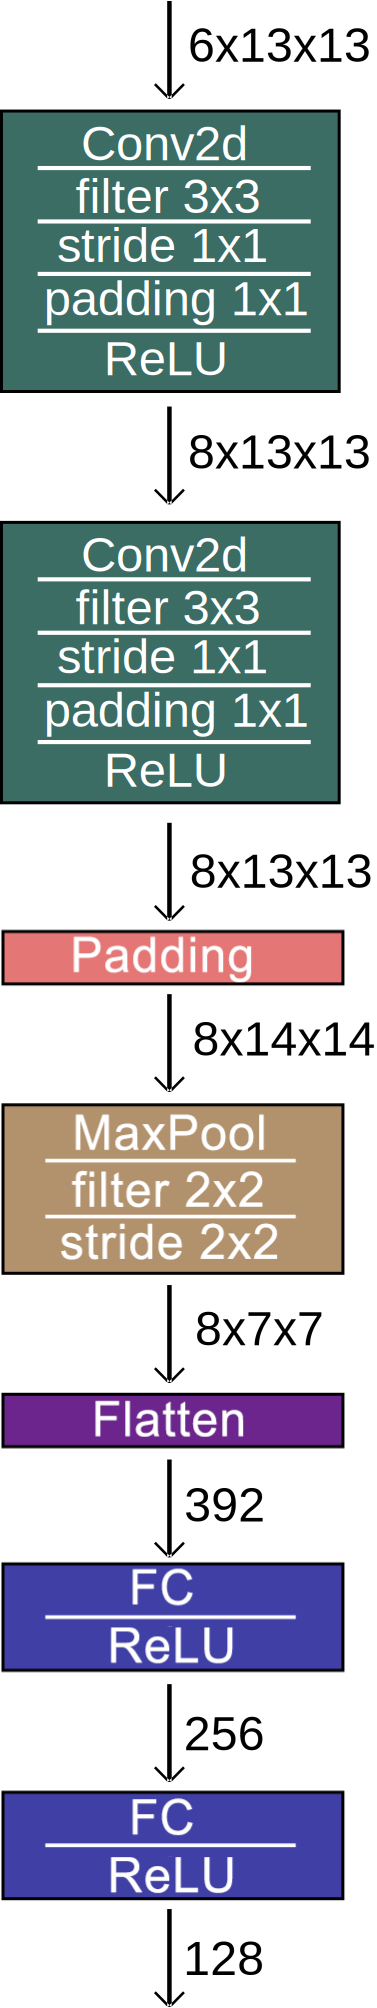
\includegraphics[width=3.0cm, height=15.5cm]{Abbildungen/ConvNet.png}
	\caption[ConvNet]{\\ConvNet}
	\label{fig:ConvNet}
\end{wrapfigure}

Im Rahmen dieser Ausarbeitung soll sich auf eine Netzstruktur konzentriert werden, um die Vergleichbarkeit der einzelnen Algorithmen zu erhöhen. Dennoch müssen, aufgrund des Algorithmus, kleinere Anpassungen an der Netzstruktur vorgenommen werden. Diese werden im weiteren erklärt.\\
Dieses NN stellt dabei einen Kompromiss zwischen Vollständigkeit und Effizienz dar. Wurden in den Papers von \cite{Autonomous_Agents_in_Snake_Game_via_DRL} und \cite{UAV} nur ein einziges großes CNN \ref{sec:Anhang_CNN} genutzt, welche Gefahr läuft viele, für den Spielerfolg, unnötige Informationen zu verarbeiten und eventuelle Probleme mit variablen Spielfeldgrößen zu bekommen, so wird in dieser Ausarbeitung auf ein zweiteilige Netzstruktur gesetzt. Diese besteht aus dem ConvNet und dem Actor-, Critic- oder Q-Head.
Zuerst wird die AV durch zwei Convolutional Layer mit einer ReLU Aktivierungsfunktion geleitet. Dabei erhöht sich die Channel-Anzahl auf acht, wobei eine weitere Erhöhung der Channel-Anzahl aufgrund der bereits sehr stark optimierten AV nicht nötig ist. Die Feature Map wird während dieses Prozesses nicht minimiert, aufgrund des Paddings der Conv2d Layers. Dies soll den Informationsverlust an den Rändern minimieren.  
Danach werden allen Feature Maps eine Null-Zeile und Spalte hinzugefügt (Padding), damit beim Max-Pooling unter der Filtergröße und dem Stride von 2x2, auch die letzten Zeile und Spalte verarbeitet wird. Der Tensor besitzt nun die Form (8x14x14). Nach dem max-pooling besitzt der Tensor, Feature Maps der Größe 7x7. Nach einer Einebnung (Flatten) zu einem eindimensionalen Tensor wird, wird dieser durch zwei weitere Fully Connected Layer (FC) mit einer ReLU Aktivierungsfunktion propagiert. Der resultierende Tensor besitzt die Größe 1x128 und ist ein zwischen Ergebnis, da dieser nun mit der SO verbunden wird (Join).
%eine zeile platz sonst failed die Formartierung
\begin{wrapfigure}{l}{5.1cm}
	\centering
	\includegraphics[width=3.0cm, height=8.0cm]{Abbildungen/Actor.png}
	\caption[Actor-Head]{\\Actor-Head}
	\label{fig:Actor_Head}
\end{wrapfigure}

Da das NN in beide Algorithmus-Arten verwendet wird, müssen Netzwerkköpfe für den Actor, Critic und für das Q-Net definiert werden. Alle unterscheiden sich jedoch nur in ihrer Ausgabe. 
Nachdem der Joined Tensor (1x169) durch zwei weitere FC Layer mit ReLU Aktivierungsfunktion propagiert wurde, benötigt der Actor des PPO-Agenten eine Wahrscheinlichkeitsverteilung über alle Actions. Daher auch die Ausgabe von einem Tensor der Größe drei. Um diese Wahrscheinlichkeitsverteilung zu erhalten, wird die SoftMax Funktion angewendet, siehe \ref{fig:Actor_Head}.\\
Der Critic des PPO verwendet hingegen den Critic-Head, siehe \ref{fig:Critic_Q_Head} links. Dieser leitet den Joined Tensor durch ein weiteres FC Layer mit ReLU Aktivierung. Der Resultierende Output wird danach durch ein weiteres FC Layer ohne Aktivierung geleitet. Da der Critic für jeden State die Discounted Sum of Rewards zu bestimmt \ref{sec:Baseline_Estimate}, gibt dieser einen Tensor mit einem einzigen Wert zurück.
Der Q-Net-Kopf ist in seinem Aufbau sehr ähnlich zu dem Critic-Kopf. Da dieser jedoch die Q-Values für jede Aktion im Zustand angeben soll, muss ein Tensor der Größe drei zurückgegeben werden. Von der Struktur des Netzes sind jedoch der Critic- und Q-Net-Kopf gleich, siehe \ref{fig:Critic_Q_Head}.
\begin{figure}[H]
	\centering
	\includegraphics[width=3cm, height=5.2cm]{Abbildungen/Critic.png}
	\hspace{.3\linewidth}% Abstand zwischen Bilder
	\includegraphics[width=3cm, height=5.2cm]{Abbildungen/QNet.png}
	\caption[Critic- und Q-Net-Head]{Darstellung des Critic-Kopfes (links) und des Q-Net-Kopfes (rechts).}
	\label{fig:Critic_Q_Head}
\end{figure}


\subsection{DQN}
Der DQN Algorithmus und damit auch die Agenten, welche auf dem Algorithmus basieren, bestehen aus drei Komponenten. Diese ermöglichen die Implementierung der Hauptmethoden act und learn.
\begin{figure}[H]
	\centering
	\def\svgscale{0.18}
	\input{Abbildungen/DQN-Agent.pdf_tex}
	\caption[DQN-Agent]{Darstellung des DQN-Agent mit seinen Komponenten.}
	\label{fig:DQN-Agent}
\end{figure}
Diese Hauptmethoden sind in der DQN-Komponente eingebettet, welche die zentrale Instanz des DQN darstellt. In ihr werden zudem die Memory und Q-Network Komponente verwaltet. Des Weiteren werden wichtige Konstanten für den DQN Algorithmus, wie z.B. Gamma (gamma), Epsilon (eps), Epsilon-Dekrementierung (eps\_dec), der minimal Wert für Epsilon (eps\_min), die Batch-Size (batch\_size), die maximale Größe des Memory (max\_mem\_size) und die Lernrate (lr), in der DQN-Komponente gespeichert.\\
Die Memory-Komponente speichert die gesammelten Erfahrungen des DQN-Agenten in einer Ring-Buffer Struktur. Sollte dieser Buffer voll sein, so werden die ältesten Erfahrungen mit den neuen überschrieben.
Die gespeicherten Erfahrungen werden im weiteren Verlauf von der learn Methode abgerufen, um mit ihnen den Lernprozess durchzuführen. Abzuspeichernde Werte, für jeden Schritt, sind dabei die around\_view (AV), die scalar\_obs (SO) die Aktion (action), der Reward (reward), die Information, ob man sich in einem terminalen Zustand befindet (terminal) und die around\_view (AV\_) und scalar\_obs (SO\_) des Nachfolgezustandes. \\
Die Q-Network-Komponente verwaltet das NN (Q-Network). Dieses wird von der act Methode dazu genutzt, um die Aktionen für das Env zu bestimmen. Des Weiteren wird das Q-Network durch die learn Methode aktualisiert, sodass eine höhere Performance erreicht werden kann.

\subsubsection{Aktionsauswahlprozess}
Zur Bestimmung der nächsten Action wird der act Methode die momentane Obs übergeben.
Diese generiert einen Zufallswert zwischen null und eins, was den Wahrscheinlichkeiten von 0\% bis 100\% entspricht.
Ist der Zufallswert größer als den momentane Epsilon-Wert, so wird die Aktion durch das Q-Network bestimmt. Anderenfalls wird eine zufällige Aktion ausgewählt. Die Bestimmung der Aktion durch das Q-Network geschieht dabei wie folgt.\\
Die around\_view (AV) und die scalar\_obs (SO) werden durch das Q-Network, entsprechende der Ausführungen in \ref{sec:Konzept_Netzstruktur}, geleitet. Dieses gibt einen Tensor der Größe drei wieder, welche die Q-Values der Aktionen turn left (0), turn right (1) und do nothing (2) beinhaltet.
Es wird daraufhin die Aktion gewählt welche dem Index des größten Q-Values entspricht.\\
Sei (0.32, -0.11, 0.45) ein Tensor, welcher vom Q-Network zurückgegeben wurde, dann würde no nothing (2) gewählt werden, da 0.45 der größte Q-Value ist und an Stelle 2 steht.\\
Zum Schluss wir die Aktion zurückgegeben und die Methode terminiert.
\begin{figure}[H]
	\centering
	\def\svgscale{0.13}
	\input{Abbildungen/DQN-Aktionsbestimmung.pdf_tex}
	\caption[DQN-Aktionsbestimmung]{Darstellung der Aktionsbestimmung des DQN-Agent.}
	\label{fig:DQN-Aktionsbestimmung}
\end{figure}

\subsubsection{Lernprozess}
Der Lernprozess wird über die learn Methode ausgeführt und stellt sich dabei wie folge dar:\\
Zuerst wird überprüft, ob im Memory genügend Experiences (Exp) gespeichert sind, um einen Mini-Batch mit der zuvor definierten batch\_size, zu extrahieren. Sollte dies nicht der Fall sein, wird die Methode terminiert. Anderenfalls wird ein Mini-Batch aus zufälligen Exp ohne Duplikate gebildet.\\
Danach wird der Q-Value bestimmt, welcher zu der abgespeicherten Aktion gehört. Es wird daher $Q(s_i,a_i;\theta_i)$ bestimmt \ref{eq:DQN_Loss}, wobei $s_i$ die Observation (AV und SO), $a_i$ die gewählte Aktion im State $s_i$ und $\theta$ die Netzwerkparameter des Q-Network, darstellten. Dieser wird als Q-Eval definiert.
Als nächstes werden die Q-Values des Nachfolgezustandes (AV\_ und SO\_) bestimmt. Sollte der Nachfolgezustand ein terminaler Zustand sein, so wird der Q-Value auf null gesetzt, da die Q-Values die zu erwartende Discounted Sum of Rewards angeben. In einem terminalen Zustand ist diese gleich null, da keine Zustande mehr Besucht werden können \ref{sec:Q-Learning}.\\
Daraufhin wird der maximale Q-Value bestimmt, mit gamma multipliziert und mit dem erhaltenen Reward addiert. Es wird daher $r(s,a) + \gamma \max_{a'}Q(s',a';\theta_{i-1})$ bestimmt \ref{eq:DQN_Loss}. Dieser Wert wird als Q-Target definiert und entspricht Q-Eval.
Am Ende wird der Mean Squared Error zwischen den Q-Targets und Q-Evals aus dem Mini-Batch gebildet. Auf Basis dieses Fehlers soll das Q-Network mittels Backpropagation und Gradientenverfahren \ref{Backprop_GD} angepasst werden.

\subsection{PPO}
\begin{figure}[H]
	\centering
	\def\svgscale{0.18}
	\input{Abbildungen/PPO-Agent.pdf_tex}
	\caption[PPO-Agent]{Darstellung des PPO-Agent mit seinen Komponenten.}
	\label{fig:PPO-Agent}
\end{figure}
Der PPO Algorithmus und damit auch die Agenten, welche auf diesem Algorithmus basieren, bestehen aus vier Komponenten. Diese ermöglichen die Implementierung der Hauptmethoden act und learn.\\
Diese Hauptmethoden sind in der PPO-Komponente eingebettet, welche die zentrale Instanz des DQN darstellt. In ihr werden zudem die Memory-, Actor- und die Critic-Komponenten verwaltet. Des Weiteren werden wichtige Konstanten für den PPO Algorithmus, wie z.B. Gamma (gamma), der Epsilon-Clip-Wert (eps\_clip) \ref{sec:Surrogate_Objectives}, Anzahl der Trainingsläufe pro Datensatz (K\_Epochs), die Lernrate (lr) und weitere Statische Konstanten, in der PPO-Komponente gespeichert.\\
Die Memory-Komponente speichert die gesammelten Erfahrungen des PPO-Agenten. Diese werden im weiteren Verlauf von der learn Methode abgerufen, um mit ihnen den Lernprozess durchzuführen. Abzuspeichernde Werte, für jeden Schritt, sind dabei die around\_view (AV), die scalar\_obs (SO) die Aktion (action), der Reward (reward), die Information, ob man sich in einem terminalen Zustand befindet (terminal) und die logarithmierte Wahrscheinlichkeit der Aktion (log\_prob). \\
Die Actor-Komponente verwaltet das Actor-NN. Dieses wird von der act Methode dazu genutzt, um die Aktionen für das Env zu bestimmen. Des Weiteren wird das Actor-NN durch die learn Methode aktualisiert, sodass eine höhere Performance erreicht werden kann.\\
Die Critic-Komponente verwaltet das Critic-NN. Dieses wird einzig von der learn Methode verwendet, um die erwartete Discounted Sum of Rewards zu bestimmen. mit dieser wird im Trainingsverlauf der Value-Loss bestimmt \ref{eq:Value_Loss}.

\subsubsection{Aktionsauswahlprozess}
Der Aktionsauswahlprozess wird durch die act Methode in der PPO-Komponente angestoßen, welche die around\_view und die scalar\_obs übergeben bekommt. Dieser werden sogleich durch das Actor-NN, welches sich in der Actor-Komponente befindet, propagiert. Der vom Actor-NN ausgegebene Tensor der Größe drei, beinhaltet eine Wahrscheinlichkeitsverteilung. Auf Basis dieser Verteilung wird die nächste Aktion bestimmt.\\
Sei (0.05, 0.05, 0.9) die Wahrscheinlichkeitsverteilung über alle Aktionen. bestimmte man 100 Aktionen unter dieser Verteilung, so würde durchschnittlich 90-mal die Aktion zwei gewählt werden. Aktion null und eins nur rund fünfmal.\\
Zum Schluss wird die Aktion zurückgegeben und die act Methode wird terminiert.

\subsubsection{Lernprozess}
Der Lernprozess des PPO wird durch die learn Methode angestoßen. Dabei wird wie folgt verfahren.\\
Zu Beginn werden die Erfahrungen, aus den gespielten Spielen, aus dem Memory (Replay-Buffer) extrahiert. Der Memory bzw. Replay Buffer befindet sich in der Memory-Komponente.\\
Um den Return \ref{sec:Return} zu erhalten, werden die einzelnen Rewards aus dem Memory, welche extrahiert worden sind, diskontiert. Sollte der Reward dabei aus einem terminalen Zustand entstanden sein, so wird dieser auf null gesetzt, da der Return der diskontierten Summe aller Rewards bis zum Ende der Spielepisode entspricht. Nach einem terminalen Zustand werden keine weiteren zustände besucht, sodass keine neuen Rewards gesammelt werden können und daher der Return gleich null ist.\\
Um ein gleichmäßigeres Lernen zu unterstützen, werden die Rewards in Anschluss noch normalisiert.
Danach wird die folgende Prozedur (K\_epochs) mal ausgeführt, um das NN zu trainieren. Danach terminiert die learn Methode.\\
Als nächstes werden die logarithmierte Wahrscheinlichkeiten für die gespeicherten Aktionen $a_i$ $\pi_{\theta}(a_{t}|s_{t})$ bestimmt \ref{sec:Probability_Ratio}. Dazu werden die aus dem Memory entnommenen AVs (around\_view) und SOs (scalar\_obs) durch das Actor- und Critic-NN propagiert. Anschließend werden die logarithmierte Wahrscheinlichkeiten für die Aktionen bestimmt und zusammen mit den Baseline Estimates \ref{sec:Baseline_Estimate} und den Entropien der Wahrscheinlichkeitsverteilungen \ref{sec:PPO_Training_Objective_Function} zurückgegeben.\\
Daraufhin werden die Probability Ratios aus der eben bestimmten logarithmierte Wahrscheinlichkeiten und den alten logarithmierte Wahrscheinlichkeiten des Memories bestimmt \ref{sec:Probability_Ratio}.
Nachfolgend werden die Advantages durch Subtraktion der Returns mit den Baseline Estimates berechnet $\hat{A}_{t}(s, a) = R_{t} - b(s_{t})$ \ref{sec:Advantages}.\\
Des Weiteren werden als nächstes die Surrogate Objective Losses Surr1: $r_{t}(\theta) \hat{A}_{t}(s, a)$ und Surr2: $\text{clip}(r_{t}(\theta), 1 - \epsilon, 1 + \epsilon) \hat{A}_{t}(s, a)$ bestimmt \ref{sec:Surrogate_Objectives}, mit welchen der Actor-Loss $L^\text{CLIP}_{t} (\theta) = \mathbb{\hat{E}}_{t} [ \min(r_{t}(\theta) \hat{A}_{t}(s, a), \text{clip}(r_{t}(\theta), 1 - \epsilon, 1 + \epsilon) \hat{A}_{t}(s, a))]$ berechnen wird.
Um zum Schluss den gesamt Loss des PPO zu bestimmen zu können, wird zusätzlich noch der Value-Loss $L^{\text{VF}}_{t} = (V_{\theta}(s_{t})-V_{t}^{targ})^2 \text{ wobei } V_{t}^{targ} = r_{t}(\theta)$ und Entropy-Loss bestimmt \ref{sec:PPO_Training_Objective_Function}. Diese wenden dann alle zusammengerechnet, entsprechend der Formel: 
$L^\text{PPO}_{t} (\theta) = L^\text{CLIP + VF + S}_{t} (\theta) = \mathbb{\hat{E}}_{t} [L^{\text{CLIP}}_{t}(\theta) - c_{1}L^{\text{VF}}_{t} + c_{2}S[\pi_{\theta}](s_{t})]$ \ref{sec:PPO_Training_Objective_Function}.\\
Das Actor- und Critic-NN werden mit dem Loss unter Zuhilfenahme von Backpropagation und Gradientenverfahren aktualisiert.

\subsection{Vorstellung der zu untersuchenden Agenten}
Ein zentraler Aspekt eines Vergleiches von verschiedenen RL-Agenten ist die genaue Definition dieser einzelnen. 
Basierende auf den Grundlagen \ref{sec:Agent} soll in diesem Abschnitt die zu vergleichenden Agenten vorgestellt werden.\\
Da die ausgewählten Hyperparameter einen immensen Einfluss auf das Verhalten der Agenten besitzen, ist ein Vergleich zwischen DQN und PPO Agenten mit wahllos gewählten Hyperparametern folglich wenig aussagekräftig. Darum sollen im weiteren die Wahl der Hyperparameter der Agenten hier begründet werden.\\
\\Wie bereits in der Abbildung \ref{fig:Vorgehen} zu erkennen ist, sollen 6 Agenten definiert und miteinander verglichen werden.
\begin{figure}[H]
	\centering
	\def\svgscale{0.102}
	\chapter{Agenten}
Ein zentraler Aspekt der eines Vergleiches von verschiedenen RL-Agenten ist die genaue Definition der einzelnen Agenten. Basierende auf den Grundlagen \ref{sec:Agent} soll in diesem Kapitel der Begriff vervollständigt und die zu vergleichenden Agenten sollen vorgestellt werden.\\
Erste statistische Erhebungen haben gezeigt, dass die ausgewählten Hyperparameter einen immensen Einfluss auf das Verhalten der Agenten haben. Bestätigt wird diese Aussage durch die Quelle \cite{Sutton1998}. Ein Vergleich zwischen DQN und PPO mit wahllos gewählten Hyperparametern ist folglich wenig aussagekräftig. Daher ist auch die Definition des Begriffs Agent, welcher nur zwischen DQN und PPO diffenenziert, unzureichend.\\
\\Angebracht wäre eine neuer erweiterte Definition des Begriffs Agent für diese Ausarbeitung. Diese soll um den entscheidenen Faktor der Hyperparameter erweitert werden. Ein Agent wird daher nicht mehr alleinig durch seine Art (Q-Learning oder Policy Gradient bzw. DQN oder PPO) definiert, sondern ebenfalls durch die ausgewählten Hyperparameter.Eine Analogie aus dem Tierreich sollte hier Klarheit verschaffen.\\
\\Im Tierreich gibt es Hunde und Katzen. Diese stellen die RL-Klassen, wie z.B. Q-Learning- oder Policy Gradient Verfahren, dar. Sieht man jedoch genauer hin, so unterscheiden sich die Hunde und Katzen durch ihre jeweiligen Rassen, wie z.B. Pudel und Dalmatiner bei den Hunden und Maine Coons und Norwegische Waldkatzen bei den Katzen. Diese stellen die Algorithmusklassen, wie z.B. DQN oder PPO, dar. Dennoch unterscheiden sich auch Hunde und Katzen der selben Rasse untereinander, nämlich in ihrer DNS. Diese stellt die letzte Differenzierungsebene der Agenten dar. Im Sachzusammenhang stellen die Hyperparameter und Attribute, wie beispielsweise die Netzstruktur, die DNS eines Agenten dar.\\
Soll nun also ein Vergleich zwischen verschiedenen Agenten vollzogen werden, so gilt es als erstes die einzelnen Agenten zu definieren, daher ihre RL-Klasse, Algorithmusklasse und Hyperparameter zu bestimmen.

\section{Agenten}
Im Folgenden werden die einzelnen Agenten, welche untereinander verglichen werden sollen, tabellarisch vorgestellt. Daher wird Aufschluss über Details, wie z.B. die RL-Klasse, Algorithmusklasse, Hyperparameter und die Netzstruktur gegeben.
\begin{longtable}[h]{|p{3.5cm}|p{2.5cm}|p{1.5cm}|p{6cm}|}
	\caption{Agenten}
	\label{tab:Agenten} 
	\endfirsthead
	\endhead
	\hline
	Agentenname & RL-Klasse & Algo-rithmus-klasse & Hyperparameter \\
	\hline
	DQN\_0.99\_64\_5e-6\_2**12\_5e-4 & Q-Learning & DQN & 
	\begin{itemize}
		\item gamma ($\gamma$) =  0.99
		\item batch\_size = 64 = $2^{6}$
		\item epsilon\_decrement = $5\mathrm{e}{-6}$
		\item max\_mem\_size = $2^{12}$
		\item lr = $5\mathrm{e}{-4}$
	\end{itemize} 
	\\
	\hline
	DQN\_0.95\_128\_1e-5\_2**13\_1e-4 & Q-Learning & DQN & 
	\begin{itemize}
		\item gamma ($\gamma$) =  0.95
		\item batch\_size = 128 = $2^{7}$
		\item epsilon\_decrement = $1\mathrm{e}{-5}$
		\item max\_mem\_size = $2^{13}$
		\item lr = $1\mathrm{e}{-4}$
	\end{itemize} 
	\\
	\hline
	PPO\_0.99\_128\_10\_1e-3\_1.5e-3\_0.5\_1e-3\_128\_2**11 & Policy Gradient & PPO & 
	\begin{itemize}
		\item gamma ($\gamma$) =  0.99
		\item K\_epochs = 10
		\item epsilion\_clip = 0.2
		\item lr\_actor = $1\mathrm{e}{-3}$
		\item lr\_critic = $1.5\mathrm{e}{-3}$
		\item critic\_loss\_coefficient = 0.5
		\item entropy\_coefficient = 0.001
		\item batch\_size = 128
		\item max\_mem\_size = $2^{11}$
	\end{itemize} 
	\\
	\hline
	PPO\_0.95\_128\_8\_0.5e-3\_1e-3\_0.5\_1e-4\_64\_2**9 & Policy Gradient & PPO & 
	\begin{itemize}
		\item gamma ($\gamma$) =  0.99
		\item K\_epochs = 10
		\item epsilion\_clip = 0.2
		\item lr\_actor = $1\mathrm{e}{-3}$
		\item lr\_critic = $1.5\mathrm{e}{-3}$
		\item critic\_loss\_coefficient = 0.5
		\item entropy\_coefficient = 0.001
		\item batch\_size = 128
		\item max\_mem\_size = $2^{11}$
	\end{itemize} 
	\\
	\hline
\end{longtable}
	\caption[Agenten]{Darstellung der zu untersuchenden Agenten.}
	\label{fig:Agenten}
\end{figure}
Der erste Agent PPO-01 soll ein langsamer aber stetiger Lerner sein. Mit einer ACTOR-LR von 2e-4 und einer CRITC-LR von 4e-4 wurden Lernraten gewählt, welche, spezifisch für diese Netzstruktur, im Mittelfeld liegen. Ein hoher Wert für GAMMA von 0.99 sorgt für ein zukunftsorientiertes Lernen. Mit einem K\_EPOCHS-Wert von acht wird das Lernen weiter verlangsamt und verstetigt. Damit der PPO-01 keine zu großen Aktualisierungen der Netze unternimmt, wurde EPS\_CLIP auf 0.15 gesetzt, was, verglichen mit der Literatur \cite[S. 6]{PPO}, recht niedrig ist.\\
\\ Der PPO-02 soll ein schnell lernendes Verhalten zeigen. Zu diesem Zweck wurden zwar niedrige Lernraten von des Actors von 1e-4 und des Critics von 2.5e-4 gewählt, jedoch sorgt relativ großer K\_EPOCHS-Wert von zwölf für ein stärkeres Aktualisieren der Netzwerkparameter von Actor und Critic. Dies wird ebenfalls durch den EPS\_CLIP-Wert von 0.25 unterstützt, welcher, nach der PPO Literatur \cite[S. 6]{PPO}, höher als der Durchschnittswert ist. Der GAMMA-Wert von 0.95 bestärkt zudem den schnelleren Lernerfolg, aufgrund der Kurzzeitpräferenz des Agenten.\\
\\PPO-03 soll ein Kompromiss zwischen schnellen Lernen und stetigem Fortschritt sein. Mit mittleren Lernraten von des Actors und Critics von 1.5e-4 bzw. 2.5e-4 sollte ein schneller und zugleich stetiger Lernfortschritt erzielt werden. Der GAMMA-Wert von 0.97 soll als Kompromiss zwischen Kurz- und Weitsichtigkeit dienen. Auch die Werte von K\_EPOCHS mit zehn und EPS\_CLIP von 0.2 werden in der Literatur \cite[Anhang A]{PPO} empfohlen und stellt ein gutes Mittelmaß dar.\\
\\Der DQN-01 ist wieder als langsamer Lerner gedacht. Mit einer mittleren LR on (LR = 0.9e-4) und einem großen GAMMA-Wert von 0.99, wird ein stetiges und zukunftsorientiert Lernen bestärkt. Eine BATCH\_SIZE und Memory-Size (MAX\_MEM\_SIZE) 64 und 2**15, soll zudem das Lernen verlangsamen. Geringe Werte für Eps\_Dec und EPS\_MIN von 5e-6 und 0.01 sollen die Neugierde des Agenten zu Beginn stärken und die Wahl von Zufallsaktionen in späteren Trainingsphasen senken.\\
\\DQN-02 ist wieder als Schnelllerner konzipiert worden. Eine vergleichsweise hohe Lernrate (LR) von 1.5e-4 in Verbindung mit einem mittleren bis kleinen Wert für Gamma von 0.95 soll einen schnellen Lernfortschritt generieren. Dies wird durch die niedrige Memory-Size (MAX\_MEM\_SIZE) von 2**11 und die große Epsilon-Dekrementierung (EPS\_DEC) von 1e-5 verstärkt. Auch sorgt der verhältnismäßig große Wert für EPS\_MIN von 0.05 für eine schnellerer Exploration und damit für ein schnelles Lernen.\\
\\ Der DQN-03 besitzt die folgenden Hyperparameter, LR = 1e-4, GAMMA = 0.97, BATCH\_SIZE = 64, MAX\_MEM\_SIZE = 2**12, 
EPS\_DEC = 8e-6 und EPS\_END = 0.025 und ist mit dieser Kombination an Parametern ein mittelfristiger Lerner.

\section{Optimierungen}
In diesem Abschnitt werden die anzuwendenden Optimierungen vorgestellt und erklärt, welche nach dem Baseline-Vergleich die Leistung in den einzelnen Evaluationskategorien noch weiter verstärken soll. Zu diesem Zweck sollen vier Optimierungen auf die Baseline Agenten (Agenten ohne Optimierungen) angewendet werden, welche aus einer verwandten Arbeit \ref{sec:Paper_1} und eigenen Ideen stammten.\\
\\ Die Optimierungen welche aus dem Paper "`UAV Autonomous Target Search Based on Deep Reinforcement Learning in Complex Disaster Scene"' \cite{UAV} konnten bezüglich ihrer Qualität nicht überzeugen. Das aper hat als Optimierung eine neue Reward Funktion vorgestellt die sehr einfach gehalten ist und wenige Spielfaktoren mit in die Berechnung des Rewards mit einfließen lasst  sodass zwei Optimierungen aus dem Paper "`Autonomous Agents in Snake Game via Deep Reinforcement Learning"' \cite{Autonomous_Agents_in_Snake_Game_via_DRL} für den folgenden Vergleich ausgewählt wurden.

\subsection{Optimierung A - Dual Experience Replay} \label{sec:Konzept_Optimierung01}
Die Idee für Dual Experience Replay oder auch hier Splited Memory genannt, stammt aus der Arbeit "`Autonomous Agents in Snake Game via Deep Reinforcement Learning"' \cite{Autonomous_Agents_in_Snake_Game_via_DRL} und wurde in \ref{sec:Paper_1} bereits erwähnt.\\
Diese Optimierung zielt darauf ab, den Replay Buffer (Memory) zu zweiteilen, sodass ein Mem1 und Mem2 entstehen. In Mem1 werden ausschließlich Erfahrungen gespeichert, welche einen Reward vorweisen können, der größer als ein vordefinierter Grenzwert ist. In Mem2 werden alle übrigen Erfahrungen gespeichert. Diese Aufteilung zielt darauf ab, dass zu beginn ein größerer Anteil an guten Erfahrungen für das Lernen verwendet wird, um das Lerntempo und die Stabilität zu erhöhen. Den Verfassern schwebt ein Verhältnis von (80\% guten und 20 \% schlechteren Erfahrungen vor). Dieses Verhältnis normalisiert sich über die Trainingszeit, daher zum Verhältnis von (50\% zu 50\%).\\
Problematisch ist jedoch die erfahrungsorientierte Aufteilung, da diese für den PPO nur schlecht umsetzbar ist.\\
Alternativ kann die Sortierung nicht auf Erfahrungsbasis, sondern Episoden basiert geschehen. Es werden daher die besten Spielepisoden, gemessen an ihren Scores, in die Memories einsortiert.\\
Zu diesem Zweck wird eine weitere Memory-Art in den Memory-Komponenten des DQN und PPO definiert, welchen diese beschriebene Funktionalität bereitstellt. Diese trägt den Namen Splited-Memory\\
Beim DQN Memory wird zusätzlich darauf geachtet, dass beim Einfügen einer ganzen Episode an Erfahrungen die Ring-Buffer Eigenschaften des Memory erhalten bleiben. Beim Memory des PPO ist dies nicht nötig.


\subsection{Optimierung B - Joined Reward Function} \label{sec:Konzept_Optimierung02}
Die Joined Reward Function wurde im Paper "`Autonomous Agents in Snake Game via Deep Reinforcement Learning"' \cite{Autonomous_Agents_in_Snake_Game_via_DRL} vorgestellt und in \ref{sec:Paper_1} erklärt. Sie setzt sich aus drei Teilen zusammen. Die Basis bildet ein Distanz Reward, welcher abhängig von der Distanz und Schwanzlänge ist. Um unerwünschte Lerneffekte, von beispielsweise der Neuerzeugung eines Apfels, zu verhindern werden diese Erfahrungen aus dem Memory gelöscht, was die Training Gap Strategy und den zweiten Teil der Reward Funktion darstellt. Zur Verstärkung des Pathfindings wird die Timeout Strategy angewendet, welche den Agenten für nicht zielgerichtetes Verhalten, wie z.B. das unnötige Umherlaufen, bestraft.\\
Die Implementierung dieser neuen Reward Funktion findet in der Reward-Komponente statt. Dabei wird der Reward wie folgt berechnet:
\begin{align}
	r_{distanz}(dis, len, size) = \frac{10}{dis} \times \frac{len}{size}
\end{align}
$dis$ stellt die Distanz gemessen mit der Euklidischen Norm dar, $len$ ist die Länge der Snake und $size$ ist die Größe des Spielfeldes (bei einer Spielfeldform von 8x8 ergibt sich eine Größe von 64).\\ Da die Training Gap Strategy zu Problemen beim PPO führen würde, wird diese nicht beachtet. Die Timeout Strategy wird in abgewandelter Form implementiert. Dies geschieht nach folgender Formel:
\begin{align}
	r_{timeout}(steps, len) = \frac{1}{100} \times \frac{steps}{len}
\end{align}
$steps$ beschreibt die Anzahl an Schritten, welche seit dem letzten Konsum eines Apfels gelaufen worden sind. 
Die Joined Reward Function lautet daher: $r_{res}(dis, len, size, steps) = 	r_{distanz}(dis, len, size) - r_{timeout}(steps, len)$.

\subsection{Optimierung C - Anpassung der Lernrate} \label{sec:Konzept_Optimierung03}
Die dritte Optimierung versucht das Lernen des Agenten durch das stetige Anpassen der Lernrate (LR) zu verbessern. 
Die Lernrate wird immer dann mit 0.95 multipliziert und als neue LR gesetzt, sobald keine Performance Steigerung in den letzten 200 Schritten erfolgt ist.

\subsection{Optimierung D - Parameteraddition zu den Netzwerken} \label{sec:Konzept_Optimierung04}
Die vierte Optimierung versucht durch das Hinzufügen von Parametern zu den Netzwerken des Actors, Critics und des Q-Networks die Performance zu steigern. Konkret sollen die Parameter der Netzwerke ansatzweise verdoppelt werden. Natürlich bietet sich dies nicht an jeder Stelle der Netzstruktur an, daher werden nur bestimmte Layer des NN von der Optimierung betroffen sein. An der Struktur des NN wird jedoch nichts verändert. Die optimierte Netzstruktur ist im Anhang \ref{fig:ConvNetOptimized} dargestellt. 

\section{Datenerhebung} \label{sec:Konzept_Datenerhebung}

\chapter{Implementierung}
Für eine Umsetzung eines solchen Vergleichs, wie er in dem Kapitel \ref{chap:Vorgehen} beschrieben worden ist, ist es nötig eine Implementierung des Spiels Snake und der beiden Agenten, inklusive der Ablaufroutine, durchzuführen. Als Programmiersprache wurde Python (3.7.9) gewählt.\\
Python bietet im Bereich des DRL eine Vielzahl an Frameworks, welche nicht nur bei der Implementierung des Envs. helfen, sondern auch welche, die Funktionalität der Neuronalen Netzwerke bereitstellen.

\section{Snake Environment}
Zur Implementierung des Spiels Snake wurde das Framework gym von OpenAI genutzt (\url{https://gym.openai.com/}). Dieses bietet viele Methoden und Vorgaben in der Projektstruktur, welche das Implementieren erleichtern. So besteht das Snake Environment Package (snake\_env), aus den wesentlichen Files:

\begin{itemize}
	\item gui
	\item observation
	\item snake\_env
	\item snake\_game
\end{itemize}

\subsection{Schnittstelle} \label{sec:Impl_Schnittstelle}
Die grundlegende Schnittstelle des Snake Env. wird in dem File snake\_env bereitgestellt. In diesem wird die Klasse SnakeEnv definiert, welche durch die Vererbung der Oberklasse gym.Env zentrale Methoden übernimmt. Zu diesen gehören die step, reset, render und close Methode.\\
Weiterhin bietet die selbst definierte Methode post\_init die Möglichkeit zentrale Einstellungen, wie z.B. die Spielfeldgröße und GUI-Aktivierung, zu editieren. 
Die step-Methode startet den Ausführungsprozess der vom Agenten ausgewählten Action, durch Aufrufen weiterer Methoden \ref{sec:Impl_Spiellogik}. Nach der Abarbeitung wird die neue Obs, der Reward, das done-flag und das has\_won-flag übermittelt, wobei letzteres zur Bestimmung des Sieges dient.
Die reset-Methode startet das Spiel von neuem. Zum Schluss wird dann noch die Obs. zurückgegeben.
Die render-Methode ruft die Methoden für die visuelle Darstellung auf.
Die close-Methode terminiert das Programm.\\
Auf Basis der oben genannten Methoden wird ersichtlich, dass es sich bei der Klasse SnakeEnv um eine Wrapper-Klasse handelt, die als Schnittstelle dient.


\subsection{Spiellogik} \label{sec:Impl_Spiellogik}
Die Spiellogik, welche durch die step-Methode \ref{sec:Impl_Schnittstelle} angestoßen wird, befindet sich im snake\_game File, welches eine Klasse namens SnakeGame definiert. Neben einigen Methoden werden im SnakeGame-Objekt auch viele spielbezogene Daten, wie z.B. das Spielfeld (ground), ein Player-Objekt (p),
ein GUI-Objekt (gui) und die Spielfeldgröße (shape), den Schrittzähler (step\_counter) und eine Hilfsvariable (has\_grown), die für die Bestimmung des Reward benötigt wird.\\
Der Weiteren werden die folgenden Methoden implementiert:
\begin{longtable}[h]{|p{4cm}|p{\linewidth - 5cm}|}
	\caption{Methoden der SnakeGame Klasse}
	\label{tab:methods_of_SnakeGame} 
	\endfirsthead
	\endhead
	\hline
	Methode & Erklärung \\
	\hline
	action & action ist für die Ausführung der Aktionen verantwortlich.\\
	\hline
	evaluate & evaluate bestimmt den, durch die Ausführung der Action, zu erhaltenden Reward.\\
	\hline
	observe & observe stößt den Generierungsprozess der Obs an, welcher ausgelagert im observation File liegt. \\
	\hline
	make\_apple & make\_apple erzeugt einen neuen Apfel auf dem Spielfeld. \\
	\hline
	reset\_snake\_game & reset\_snake\_game setzt den Spielfortschritt zurück und startet es von neuem. \\
	\hline
	max\_snake\_length (getter) & Gibt die maximale Länge der Snake zurück. \\
	\hline
	is\_done (getter) & Liefert den Lebensstatus (player.done). \\
	\hline
\end{longtable}

Zum Erhalt eines tieferen Verständnisses über die Spiellogik, soll diese exemplarisch erläutert werden. Bevor dies jedoch geschehen kann muss noch die Datenhaltungsklasse Player erwähnt werden, die ebenfalls im Snake\_game File definiert ist.
Diese speichert spielerbezogen Daten, wie z.B. die Position aller Schwanzglieder inkl. des Kopfes (pos, tail), Blickrichtung (direction), die Anzahl der Schritte seit dem letzten Fressen (inter\_apple\_steps), den Lebensstatus (done) und einige Konstanten, welche für die Visualisierung benötigt werden (id, c\_s und c\_h). Zuzüglich besitzt die Player Klasse noch eine player\_reset Methode und einige getter Methoden.\\

Da Snake ein zweidimensionales Spiels ist, wird eine gleich dimensionale Matrix (ground) zur Spieldarstellung verwendet.
So kann mit dn Zeilen- und Spaltenindexen der Matrix die Position der Snake deutlich gemacht werden. So wird der Schwanz mit der Konstante c\_s, der Kopf mit c\_h, der Apfel mit -2 und das Ende der Snake mit -1, in der Matrix (ground) deutlich gemacht.
Der Einfachheit halber werden die Zeilen- und Spaltenindexe, daher die Position, ebenfalls noch in einer List (tail) festgehalten. Dieser erleichtert später die Feststellung des Lebensstatus (done).\\
\\Mit dem folgenden Aktivitätsdiagramm soll der Fokus weiter auf die action-Methode gelegt werden. Diese wird wie folgt abgearbeitet.
Als erstes wird der inter\_apple\_steps erhöht. Sollte dieser Zähler größer als, die vorher definierte, Obergrenze sein, so wird der Lebensstatus auf tot gesetzt (p.done = True) und die Methode wird terminiert. Im weiteren Verlauf wird diese Unterprozedur Abbruchprozedur genannt.\\
Anderenfalls wird als nächstes überprüft, um welche action es sich handelt, wobei die actions mit den Zahlen von null - zwei kodiert sind.
\begin{longtable}[h]{|p{4cm}|p{\linewidth - 5cm}|}
	\caption{Kodierung der Actions}
	\label{tab:Aktionscodierung} 
	\endfirsthead
	\endhead
	\hline
	Action & Erklärung \\
	\hline
	0 & Die Snake ändert ihre Richtung um 90° nach links. Z.B. Von N $\longrightarrow$ W \\
	\hline
	1 & Snake ändert ihre Richtung um 90° nach rechts. Z.B. Von N $\longrightarrow$ O \\
	\hline
	2 & Die Richtung der Snake wird nicht verändert. \\
	\hline
\end{longtable}
Entsprechende der Action wird die direction des Players angepasst. Die vier Himmelsrichtungen werden dabei mit den Zahlen von 0 - 3 dargestellt, wobei null Norden entspricht eins Osten usw.\\
Nach der Manipulation der direction des Players, wird pos, also die vorläufige neue Position, im Player-Objekt angepasst. 
Diese Änderung wird jedoch noch nicht sofort in die Matrix übertrage, da das Eintragen on Positionen außerhalb des Spielfeldes zu Fehlern führen würde. Es muss daher erst überprüft werden, ob die neue Position des Players im Spielfeld liegt. Sollte dies nicht der Fall sein, so wird die Abbruchprozedur aufgerufen.\\
Anderenfalls wird die neue Position in tail eingefügt.\\
Zu diesem Stand der Abarbeitung ist es möglich, dass das Spiel bereits gewonnen ist. Um dies zu überprüfen, wird die Länge der Snake mit der maximal möglichen Länge, welche sich durch die Spielfeldgröße ergibt, verglichen. Entspricht die Länge Snake der maximal mögliche, so wird die Abbruchprozedur aufgerufen.
Ansonsten muss als nächster Schritt die Matrix aktualisiert werden. Jedoch muss vorher festgestellt werden, ob die Snake einen Apfel gefressen hat.\\
Sollte sie dies getan haben, so wird die neue Position des Kopfes in die Matrix eingepflegt, ein neuer Apfel wird auf einer zufälligen freien Stelle generiert, inter\_apple\_steps wird auf null und die Hilfsvariable has\_grown wird auf True gesetzt. Letztere wird von der evaluate Methode verwendet, um di Höhe des rewards zu bestimmen, siehe \ref{sec:Impl_Reward_Function}.\\
Ist die Snake jedoch nicht gewachsen, so wird das letzte Schwanzglied aus Matrix und Liste gelöscht, um den Anschein von Bewegung zu erwecken. Zuzüglich wird  die Hilfsvariable has\_grown auf False gesetzt.\\
Zum jetzigen Zeitpunkt besteht immer noch die Möglichkeit, dass die Snake in sich selber gelaufen ist. Um dies festzustellen, wird tail auf Duplikate überprüft. Sollten sich Duplikate in tain befinden, wird die Abbruchprozedur aufgerufen.\\
Ansonsten wird zum Schluss noch über tail iteriert und die korrespondierenden Einträge der Matrix (ground) werden mit den Positionen von tail aktualisiert, wobei der Kopf und das letzte Schwanzglied mittels eines anderen Zahlenwert dargestellt werden.

\subsection{Reward Function} \label{sec:Impl_Reward_Function}
Die evaluate Methode, welche den Reward bestimmt, befindet sich in der SnakeGame Klasse. Basierend auf dem letzten Zug wird in dieser Methode der Reward bestimmt. Dies geschieht nach folgenden Vorbild.
Der Reward ist abhängig von drei Faktoren. Dem Fressen eines Apfels, dem Sieg und dem Verlust. Sollte keiner dieser genannten Faktoren eintreten, wird ein Reward von -0.01 zurückgegeben. Dies hält den Agenten dazu an den kürzesten Pfad zum Apfel zu finden, da jeder Schritt geringfügig bestraft wird.\\
War es der Snake möglich einen Apfel zu fressen so wird ein Reward von +1.0 zurückgegeben, da ein Sub-Goal erfüllt worden ist.
Sollte die Snake gestorben sein, durch das Verlassen des Spielfeldes oder das Laufen in sich selbst oder das zu lange Umherlaufen, so wird ein Reward von -10 zurückgegeben, um dieses Verhalten in seiner Häufigkeit zu minimieren.
Hat die Snake alle Äpfel gefressen, sodass das gesamte Spielfeld mit der Snake ausgefüllt ist, so wird ein Reward von +10 zurückgegeben, um ein solches Verhalten in seiner Häufigkeit zu maximieren.

\subsection{Observation}
Die Observation, welche das Snake Env. zurückgibt besteht aus zwei Teilen, der around\_view (AV) und der scalar\_obs (SO). Zur Erstellung der Obs wird die observe Methode in der SnakeGame Klasse aufgerufen. Diese ruft ihrerseits die make\_obs Funktion auf, welches im observation File definiert ist. Mit Hilfe verschiedener Unterfunktionen wird dann die Obs generiert.\\
Die AV lässt sich dabei als ein Ausschnitt der Matrix (ground) beschreiben, welche einen festen Bereich um den Kopf der Snake abdeckt.
Strukturen wie Wände und Teile des eigenen Schwanzes, welche vielleicht eine Sackgasse aufspannen, werden deutlich. Numerische ist die AV eine one-hot-encoded Matrix der Form (6x13x13).\\
\\Das One-Hot-Encoding benutzt zum codieren nur null und eins. Sollte ein Merkmal vorhanden sein, so wird dieses mit eins codiert anderenfalls mit null.\\
Dies ist auch der Grund, warum die AV Matrix sechs Channel (zweidimensionale Schichten) besitzt. Diese geben Aufschluss über folgende Informationen:
\begin{longtable}[h]{|p{4cm}|p{\linewidth - 5cm}|}
	\caption{Channel-Erklärung der Around\_View (AV)}
	\label{tab:around_view} 
	\endfirsthead
	\endhead
	\hline
	Channel der Matrix bzw. Erste Dimension (Ax13x13) & Erklärung \\
	\hline
	A = 0 & Die erste Feature Map signalisiert den Raum außerhalb des Spielfelds. Nährt sich die Snake dem Rand, so würde der Ausschnitt der AV aus dem Spielfeld herausragen und den Eindruck erwecken, dass dieser größer wäre als er in Realität wirklich ist. Darum werden Felder der AV, die sich außerhalb des Spielfeldes befinden, angezeigt.\\
	\hline
	A = 1 & Diese Feature Map stellt alle Schwanzglieder mit Ausnahme des Kopfes und es letzten Schwanzgliedes dar. \\
	\hline
	A = 2 & In dieser Feature Map wird der Kopf der Snake dargestellt. \\
	\hline
	A = 3 & Damit gegen Ende des Spiels der Agent noch freie Felder erkennen kann, wird in dieser Feature Map jedes freie und sich im Spielfeld befindliche Feld mit eins codiert. \\
	\hline
	A = 4 & Die vorletzte Feature Map codiert das Schwanzende der Snake. \\
	\hline
	A = 5 & In der letzte Feature Map wird der Apfel abgebildet. \\
	\hline
\end{longtable}
Vorteilhaft an der AV ist, dass, im Gegensatz zu den verwandten Arbeiten \ref{sec:Paper_1} und \ref{sec:Paper_3}, nicht das gesamte Feld übertragen wurde sondern nur der wichtigste Ausschnitt, was die Menge an zu verarbeiten Daten drastisch reduzieren kann. Des Weiteren ergeben sich keine Probleme mit der Input-Size der Convolutional Layer.\\
Ein Nachteil dieser Obs ist jedoch die Vollständigkeit. Sollte der blaue Punkt in \ref{fig:Observation} außerhalb des grauen Kasten und daher außerhalb der AV liegen, so besitzt der Agent keine Informationen über den Aufenthaltsort des Apfels.
Auch Informationen wie z.B. der Hunger, also die verbleibenden Schritte bis das Spiel endet, die Distanzen zu den Wänden und zu exkludierten Schwanzteilen und die Blickrichtung (direction) der Snake.
\begin{figure}[H]
	\centering
	\def\svgscale{0.95}
	\input{Abbildungen/Observation.pdf_tex}
	\caption[Observation]{Partielle Darstellung der verwendeten Observation. Das blaue Rechteck und dessen Schwanz stellt die Snake dar, wobei das rot umrandete Rechteck den Kopf darstellt. Die schwarzen Felder werden nicht von der AV abgedeckt, graue liegen innerhalb der AV. 
	Die gelben gestrichelten Linien stellen ein X-Ray Distanzbestimmung dar. Der blaue Kreis stellt den Apfel dar und der grüne viertel Kreis oben links symbolisiert Hunger.}
	\label{fig:Observation}
\end{figure}
Aus diesem Grund wurde die AV mit der scalar\_obs (SO) ergänzt. Diese beinhaltet skalare Informationen und ist eine Konkatenation aus X-Ray Distanzbestimmung, Hunger- Blickrichtungsanzeige und zwei Kompasse für die relative Positionsinformation zwischen Kopf und Apfel bzw. letztem Schwanzglied.
Letztere sind eindimensionale Vektoren, welche über das One-Hot-Encoding anzeigen, ob sich das gesucht Objekt relativ zum Kopf oberhalb, unterhalb oder in der selben Zeile (Matrixsicht) befindet. Analog verhält es sich mit der vertikalen Sicht.\\
Die Blickfeldanzeige ist ebenfalls one-hot-encoded und stellt mit seinem Vektor die vier Ausrichtungen Norden, Osten, Süden und Westen dar.
Da der Hunger bei einer großen Differenz zwischen inter\_apple\_steps und max\_steps einen kleinen und bei einer geringen Differenz einen großen Einfluss besitzen soll, wurde die Differenz durch eins geteilt. Nähren sich die beiden Werte, so rückt der resultierende näher an unendlich, da den Nenner immer kleiner wird. Um mit der Unendlichkeit auftretende Probleme zu umgehen wir zwei zurückgegeben, wenn die Differenz null ist.\\
In ähnlicher Weise wird mit den X-Rays Distanzbestimmungen verfahren. Bei ihnen handelt es sich um acht Distanzmesserlinien, die in 45° Abständen ausgesandt werden, siehe \ref{fig:Observation}. Befindet sich das gesucht Objekt in dieser Linie, so wird die durch eins dividierte Differenz zwischen Kopf und Objekt zurückgegeben. Es wird nach Wänden, dem eigenem Schwanz und dem Apfel gesucht. Daher wird die X-Ray Distanzbestimmung in einem Vektor der Größe 24 (3 * 8 = 24) gespeichert.

\subsection{Graphische Oberfläche}
Im gui File wird eine Klasse GUI definiert, welche das Spiel mit Hilfe des Frameworks pygame (\url{https://www.pygame.org/}) darstellt. Dazu wird in der GUI-Klasse ein Oberfläche (screen) erzeugt, welche die Matrix ground darstellt, siehe \ref{fig:Game_of_Snake}. 
Die Methode update\_GUI, welche von der SnakeGame Methode view aufgerufen wird, überschreibt dazu jeden einzelnen Eintrag des pygame-Spielfelds mit dem korrespondierenden Wert von ground. 
Spielfeld (GUI) und Matrix sind daher nicht direkt gekoppelt sondern müssen über update\_GUI angeglichen werden.\\
Die Fenstergröße der Spieloberfläche wird dynamisch berechnet und kann über das Attribut Particle verändert werden, welches die Feldgröße eines einzelnen Matrixeintrags darstellt. 
Die draw Methode ist für das Generieren der einzelnen Spielfeld-Rechtecke zuständig und reset\_GUI versetzt das Spielfeld zurück in den Ursprungszustand.


\section{Agenten}
Dieser Teil der Implementierung soll sich mit den Agenten befassen. Dabei wird näher auf die Netzstruktur, den Aktionsauswahlprozess die Lern-Methode, den Speicher (Replay Buffer) und die Hauptausführungsmethode (main Methode) eingegangen.

\subsection{Netzstruktur} \label{sec:Impl_Netzstruktur}
Zu Beginn soll die Netzstruktur erklärt werden, wobei dies unabhängig von den Agenten geschehen kann, da sowohl DQN als auch PPO Agenten das annähernd gleiche Netz nutzen.
\begin{figure}[H]
	\centering
	\def\svgscale{0.80}
	\input{Abbildungen/BaseNet.pdf_tex}
	\caption[BaseNet]{Darstellung des BaseNet, welches als Standard für den weiteren Vergleich dient.}
	\label{fig:Netzsturktur}
\end{figure}
Aufgrund der Agentenunabhängigkeit, ist das NN als eine eigenständige Klasse im base File, welches sich im common Package befindet, ausgelagert. 
Diese BaseNet-Klasse besitzt eine forward Methode, welche die Obs (AV, SO), nach dem umwandelt in Tensoren, durch das NN propagiert und einen Output bestimmt. Dieser Prozess geschieht dabei folgendermaßen:\\
Zuerst wird die AV durch zwei Convolutional Layer mit einer ReLU Aktivierungsfunktion durch propagiert. Dabei erhöht sich die Channel-Anzahl auf 32, um eine bessere Merkmalextraktion zu erhalten. Die Feature Map wird während dieses Prozesses von 13x13 auf 9x9 minimiert, was ein Effekt der Convolutional Layern ist. 
Danach werden allen Feature Maps eine Null-Zeile und Spalte hinzugefügt (Padding), damit beim Max-Pooling unter der Filtergröße und dem Stride von 2x2, auch die neunte Zeile und Spalte verarbeitet wird. Der Tensor besitzt nun die Form (30x10x10) 
Nach dem max-pooling besitzt der Tensor weiterhin 32 Channel mit Feature Maps der Größe 5x5. Nach der Ebnung (Flatten) des Tensoren zu einem eindimensionalen Tensor-Vektor wird dieser durch zwei weitere Fully Connected Layer (FC) mit einer ReLU Aktivierungsfunktion durch propagiert. Der resultierende Tensor besitzt die Größe 1x128 und ist ein zwischen Ergebnis, da dieser nun mit der SO verbunden wird (Join).\\
Da das NN in beide Algorithmus-Arten verwendet werden soll, müssen drei unterschiedliche Netzwerkköpfe definiert werden, siehe \ref{fig:Netzsturktur} rechts. Alle unterscheiden sich jedoch nur in ihrer Ausgabe. Nachdem der Joined Tensor (1x128) durch zwei weitere FC Layer propagiert wurde, benötigt der Actor des PPO-Agenten eine Wahrscheinlichkeitsverteilung über alle Actions. Daher auch die Ausgabe von einem Tensor der Größe 3 nach dem zweiten FC Layer auf welchen danach noch SoftMax angewendet wird, siehe \ref{fig:Netzsturktur} rechts oben.\\
Die Critics der PPOs und die DQNs verwendet den rechts unten dargestellten Netzwerkkopf (ValueNet-Head) \ref{fig:Netzsturktur}. Beim den Critics werden Tensoren mit einem einzigen Zahlenwert (Return) zurückgegeben, wohingegen bei den DQNs Tensoren mit drei Zahlenwerten entsprechende der Actions zurückgegeben.


\subsection{DQN}
Der DQN Algorithmus ist einer der beiden Algorithmus-Arten, welche im Rahmen dieser Ausarbeitung, implementiert wurden. Diese Implementierung findet hauptsächlich in vier Files statt, welche im dqn Package liegen, dass wiederum zum agents Package gehört.
Im dqn File wird die Agentenklasse definiert, welche die Aktionsbestimmungsmethode act und die lern Methode enthält. 
Im memoryDQN File wird die Memory-Klasse definiert, welche den Replay-Buffer darstellt \ref{sec:Q-Learning}. 
Die Files dqn\_train und dqn\_play beinhalten die eigentlichen main-Methoden, welche Agenten und Env. erstellen und den Trainings- bzw. Spielprozess umsetzt.

\subsubsection{Aktionsauswahlprozess}
Zur Bestimmung der nächsten Action wird der act Methode die momentane Obs übergeben.
Die Bestimmung der Actions durch den DQN Agenten ist maßgeblich vom $\epsilon$ Wertes abhängig \ref{alg:DQN}, welcher das Verhältnis zwischen der Wahl einer zufälligen und einer NN-basierten Action bestimmt. Dabei wird folgendermaßen vorgegangen \ref{alg:DQN}.
Zuerst wird ein Zufallswert $rand$ zwischen null und eins generiert, welcher mit $\epsilon$ verglichen wird. Wenn $rand < \epsilon$ so wird die Action mittels des NN bestimmt. Anderenfalls wird eine zufällige Action gewählt.
Zur NN-basierten Bestimmung der Action werden aus der Obs zwei Tensoren generiert, welche zum vordefinierten Device (CPU oder GPU) geschickt werden. Danach folge die Prozedur, welche in \ref{sec:Impl_Netzstruktur} dargestellt ist.

\subsubsection{Trainingsprozess}
Der Trainingsprozess wird über die learn Methode ausgeführt und stellt sich dabei wie folge dar:\\
Zuerst wird überprüft, ob im Memory genügend Experiences (Exp) gespeichert sind, um einen Mini-Batch mit der zuvor definierten batch\_size, zu extrahieren. Sollte dies nicht der Fall sein, wird die Methode terminiert. Anderenfalls wird ein Mini-Batch aus zufälligen Exp. ohne Duplikate gebildet.\\
\\Das Memory (Replay Buffer) wird durch Tensoren dargestellt, welche die Erfahrungen in einer zusätzlichen Dimension speichern. So besitzt der Tensor der AV die Form (max\_mem\_size, 6, 13, 13). Die Tensoren werden dabei wie eine Überlaufliste verwaltet, sodass wenn die Anzahl an Exp die max\_mem\_size überschreitet, die ältesten Einträge durch die neuen ersetzt werden.\\
\\Danach folgt die Bestimmung aller Q-Values der States (s) des Mini-Batch, wobei der Q-Value der zum State (s) gespeicherten Action entnommen und als q\_eval, gespeichert wird. 
Anschließend werden alle Q-Values der Nachfolge-States (s\_next) bestimmt und als q\_next gespeichert. Die Q-Values terminaler States werden anschließend auf null gesetzt, da die Discounted Sums of Rewards bis zum Ende der Spielepisode null entspricht, siehe \ref{sec:Q-Learning}.\\
Um nun q-target zu bestimmen, werden die maximalen Q-Values der s\_next bestimmt, diskontiert und mit dem, im Mini-Batch gespeicherten, Reward addiert, siehe \ref{eq:DQN_Loss}.
Nachfolgend wird der MSE (Mean Squared Error) zwischen q\_eval und q\_target bestimmt. Zuletzt wird der Fehler Mit Hilfe des Pytorch Frameworks mit Hilfe von Backpropagation und Gradient Descent \ref{Backprop_GD} zurück propagiert und entsprechend die Parameter des NN angepasst.

\chapter{Evaluation} \label{chap:Evaluation}
In diesem Kapitel sollen die Ergebnisse der angewendeten Methodik präsentiert werden. Des Weiteren wird eine Abdeckungsanalyse durchgeführt, um zu beurteilen, welche Anforderungen umgesetzt wurden. Sollen einige nicht umsetzbar gewesen sein, so werden diese erläutert.

\section{Ergebnisevaluation der Vergleiche} \label{sec:Evaluation_Ergebnisevaluation}
In der Evaluation sollen die Ergebnisse, welche aus den Vergleichen stammten, präsentiert werden.

\subsection{Evaluation der Baseline Vergleiche}
Basierend auf dem Vorgehen \fullref{sec:Konzept_Vorgehen} wird mit den Baseline Vergleichen begonnen. Bei diesen handelt es sich um die Vergleiche, welche von  nicht optimierten Agenten (Baseline Agenten) durchgeführt worden sind \fullref{fig:Konzept_Agenten}). Diese Agenten wurden in einem Trainingsverlauf, entsprechend der Beschreibung im \autoref{subsec:Konzept_Datenerhebung}, trainiert. 
Währenddessen wurden die Trainingsdaten erhoben, die grafisch dargestellt wurden. 
Als nächster Schritt wurden die Testdaten ermittelt, welche im Folgenden tabellarisch ausgewertet werden mit Ausnahme der Robustheit und Effizienz. Bei diesen bietet sich eine grafische Auswertung der Testdaten an.

\subsubsection{Performance}
Die Baseline Vergleichsauswertung soll mit der Performance beginnen. Dabei ist in der \autoref{fig:Evaluation_Baseline_01_performance} die durchschnittliche Performance bzw. Apfelanzahl der letzten 200 Epochs pro Epoch abgebildet.\\
Die DQN Agenten waren in den Vergleichen nicht in der Lage, eine durchschnittliche Apfelsammelrate von 30 Äpfeln pro Spiel zu erreichen. 
Eine vermutliche Erklärung warum die Agenten des DQN Algorithmus keine guten Leistungen erzielen konnten, liegt in der Wahl von Zufallsaktionen. Die Komplexität des Spiels Snake steigt gegen Ende immer weiter an, da die Snake mit zunehmenden Spielfortschritt keine nicht zielführenden Schritte mehr gehen darf. In einer beengten Spielsituation könnte jeder falsche Schritt zum Tod führen, wobei durch zufällige Aktionen falsche Schritte durchgeführt werden könnten. Dadurch, dass das Spiel immer vorzeitig beendet würde, könnte der DQN Agent auch seine Leistung nicht weiter steigern, weil ihm die Daten zum Lernen fehlen würden.
\begin{figure}[H]
	\centering
	\includesvg[scale=0.4517]{baseline-performance}
	\caption[Performance - Auswertung der Trainingsdaten der Baseline Vergleiche]{Trainingsdatenauswertung der Baseline Vergleiche für die Performance. Die Performance ist als Apfelanzahl pro Epoch definiert. Für einen besseren Kurvenverlauf wird die durchschn. Performance der letzten 200 Epochs abgebildet.}
	\label{fig:Evaluation_Baseline_01_performance}
\end{figure}
Im Training konnten besonders die Leistungen der PPO Agenten PPO-03 und PPO-01 überzeugen. 
Der PPO-03 kann dabei besonders mit seinem schnellen Lernerfolg punkten, wohingegen der PPO-01 mit seiner annähernd linearen Stetigkeit überzeugen kann.
PPO-02 konnte zwar ebenfalls eine fast lineare Steigerung seiner Performance erzielen, jedoch konvergierte dieser früher als der PPO-01.
Dieses Verhalten der Agenten entspricht den Darstellungen im \autoref{subsec:Konzept_Vorstellung_Agenten}.
\begin{longtable}[H]{|p{4.5cm}|p{4.5cm}|p{4.5cm}|}
	\hline
	Agent & Durchschn. Performance & Standardabweichung \\
	\hline
	DQN-01 & 17.7812 & 2.9577 \\
	\hline
	DQN-02 & 26.4226 & 4.3482 \\
	\hline
	DQN-03 & 25.4506 & 4.8280 \\
	\hline
	PPO-01 & 44.4544 & 19.6957 \\
	\hline
	PPO-02 & 38.7325 & 11.5756 \\
	\hline
	PPO-03 & 46.4268 & 14.0280 \\
	\hline
\caption{Testdatenauswertung der Baseline Vergleiche für die Performance.}
\label{tab:Evaluation_Testdaten_Performance} 
\end{longtable}
\newpage
Auch die Auswertung der Testdaten \fullref{tab:Evaluation_Testdaten_Performance} zeigt den sich in den Trainingsdaten abzeichnenden Trend. So erbringt der PPO-03 die beste und der PPO-01 die zweitbeste Leistung. Die Standardabweichungen des PPO-03 und PPO-01 zeigen jedoch, dass die Leistungen nicht konsistent sind. Besonders PPO-01 zeigte eine schwankende Performance, welche auch in den Trainingsdaten \fullref{fig:Evaluation_Baseline_01_performance} zu beobachten ist.
Daher bleibt der PPO-03 für das Evaluationskriterium der Performance der Sieger.\\
Stark mit der Performance korrelierend, stellt die Siegrate das nächste zu untersuchende Evaluationskriterium dar.

\subsubsection{Siegrate} \label{subsubsec:Evaluation_Siegrate}
Ähnlich wie bei der Performance verhält es auch mit dem Evaluationskriterium der Siegrate. PPO-03 und PPO-01 besitzen die besten Siegraten während des Trainings \fullref{fig:Evaluation_Baseline_winrate}.
\begin{figure}[H]
	\centering
	\includesvg[scale=0.4517]{baseline-siegrate}
	\caption[Siegrate- Auswertung der Trainingsdaten der Baseline Vergleiche]{Trainingsdatenauswerten der Baseline Vergleiche für die Siegrate. Für den besseren Kurvenverlauf wird die durchschn. Siegrate der letzten 200 Epochs abgebildet.}
	\label{fig:Evaluation_Baseline_winrate}
\end{figure}
Die DQN Agenten sind nicht in der Lage gewesen Siege zu erreichen und fallen daher aus der Betrachtung heraus.
Der PPO-02 zeigt eine deutlich geringe Siegrate, trotz ähnlicher Performances zu den anderen PPO Agenten.
Bemerkenswert ist des Weiteren, dass der PPO-03 zwar ähnliche Leistungen wie der PPO-01 erreicht \fullref{fig:Evaluation_Baseline_01_performance}, jedoch der PPO-01 eine deutlich bessere Siegrate erzielt. Dies ist möglicherweise auf den stetigen Lerncharakter des Agenten zurückzuführen \fullref{subsec:Konzept_Vorstellung_Agenten}.
Auch die Testdaten in \autoref{tab:Evaluation_Testdaten_Winrate} zeigen, dass PPO-01 der Sieger ist, wobei sich der eben beschriebene Trend aus den Trainingsdaten in den Testdaten widerspiegelt. Daher ist der PPO-01 der Sieger für das Evaluationskriterium der Siegrate.
\newpage
\begin{longtable}[H]{|p{4.5cm}|p{4.5cm}|p{4.5cm}|}
	\hline
	Agent & Durchschn. Siegrate & Standardabweichung \\
	\hline
	PPO-01 & 0.6759 & 0.33306 \\
	\hline
	PPO-02 & 0.0926 & 0.20478 \\
	\hline
	PPO-03 & 0.3316 & 0.32751 \\
	\hline
	\caption{Testdatenauswertung der Baseline Vergleiche für die Siegrate.}
	\label{tab:Evaluation_Testdaten_Winrate} 
\end{longtable}

\subsubsection{Robustheit} \label{subsubsec:Evaluation_Robustheit}
Die Robustheit stellt ein besonderes Evaluationskriterium dar, denn sie wird ausschließlich aus Testdaten bestimmt. Diese werden zur besseren Übersicht in eine Grafik überführt. Die Robustheit ist als durchschn. Apfelanzahl dividiert durch die Spielfeldgröße pro Quadratwurzel aus der Spielfeldgröße definiert. 
\begin{figure}[H]
	\centering
	\includesvg[scale=0.4517]{baseline-robustheit}
	\caption[Robustheit - Auswertung der Testdaten der Baseline Vergleiche]{Testdatenauswertung der Baseline Vergleiche für die Robustheit. Diese wird als durchschn. Apfelanzahl dividiert durch die Spielfeldgröße pro Quadratwurzel aus der Spielfeldgröße dargestellt.}
	\label{fig:Evaluation_Baseline_Robustheit}
\end{figure}
Wie in \autoref{fig:Evaluation_Baseline_Robustheit} zu erkennen ist, zeigen die DQN Agenten keine guten Resultate.
Sie erreichen auf kleineren Spielfeldgrößen bessere Ergebnisse als auf der Standardspielfeldgröße von 8x8. Sollte sich jedoch das Spielfeld vergrößern, so stagnieren ihre Leistungen.
Bei den PPO Agenten zeigt sich ein ähnliches Bild. Ihre Leistungen steigen ebenfalls nicht mit dem sich vergrößernden Spielfeld an. Jedoch ist der PPO-03 in der Lage, die besten Ergebnisse in den unbekannten Gebieten zu erzielen.\\
Bemerkenswert ist des Weiteren, dass sich ein Trend abzeichnet, nachdem Agenten auf geraden Spielfeldgrößen (z.B. (6x6), (8x8) und (10x10)) bessere Leistungen erzielen können als auf ungeraden (z.B. (7x7) und (9x9)).\\
Aus diesem Vergleich geht dennoch der PPO-03 Agent als Sieger für das Evaluationskriterium der Robustheit hervor.

\subsubsection{Effizienz} \label{sec:Evaluation_Effizienz_Baseline}
Die Effizienz stellt zusammen mit der Robustheit ein besonderes Evaluationskriterium dar. Sie ist als durchschn. Schrittanzahl pro Apfelanzahl definiert.
\begin{figure}[H]
	\centering
	\includesvg[scale=0.4517]{baseline-effizienz}
	\caption[Effizienz - Auswertung der Trainingsdaten der Baseline Vergleiche]{Trainingsdatenauswertung der Baseline Vergleiche für die Effizienz. Diese ist als durchschn. Schrittanzahl pro Apfelanzahl dargestellt.}
	\label{fig:Evaluation_Baseline_Effizienz}
\end{figure}
Wie in der \autoref{fig:Evaluation_Baseline_Effizienz} zu erkennen ist, sind DQN-01 und DQN-02 diejenigen, welche die wenigsten Schritte für die jeweilige Apfelanzahl unternehmen müssen. Dies gilt jedoch nicht kontinuierlich. Denkbar wären daher die DQN Agenten in Einsatzgebieten mit wenigen Zielen aber großen Distanzen einzusetzen, sodass der Effizienzcharakter der Agenten hilft beispielsweise Kraftstoff bzw. Energie zu sparen.
Eine weitere Betrachtung der DQN Agenten unter dem Kriterium der Effizienz wird jedoch aufgrund der fehlenden Daten nicht durchgeführt.
Da die DQN Agenten ausgeschieden sind, bleiben nur noch die PPO Agenten. Diese verfügen über den gesamten Trainingslauf eine solide Effizienz.
Der PPO-02 konnte bei der Auswertung der Trainingsdaten die besten Ergebnisse erzielen, gefolgt vom PPO-03.\\
Erwähnenswert ist ebenfalls, dass die Effizient-Differenz zwischen den PPO Agenten gegeben Ende deutlich abnimmt, da durch die Gesetzmäßigkeiten des Spiels Snake, kaum effizientere Routen zum Apfel zu finden sind.\\
Auch bei der Auswertung der Testdaten wird dieser Trend deutlich, wobei
einzelnen Graphen in der \autoref{fig:Evaluation_Effizienz2_Baseline} immer wieder Abschnitte besitzen, in welchen der Graph abbricht. Dies bedeutet, dass der Agent eine solche Anzahl an Äpfeln nie erreicht hat. Dies muss nicht negativ ausgewertet werde.\\
Die gute Effizienz des PPO-02 kann dabei unter anderem auf den niedrigen Gammawert von 0.93 zurückgeführt werden, welcher den Agenten dazu anhält, schnell viele gute Rewards zu erzielen \fullref{subsec:Konzept_Vorstellung_Agenten}. Da der PPO-02 sowohl in den Trainingsdaten als auch in den Testdaten bessere Ergebnisse als seine Konkurrenten zeigt, ist dieser der Sieger des Evaluationskriteriums der Effizienz.
\begin{figure}[H]
	\centering
	\includesvg[scale=0.4517]{baseline-effizienz2}
	\caption[Effizienz - Auswertung der Testdaten der Baseline Vergleiche]{Testdatenauswertung der Baseline Vergleiche für die Effizienz.}
	\label{fig:Evaluation_Effizienz2_Baseline}
\end{figure}

\subsection{Evaluation der Optimized Vergleiche}
Nach der Durchführung der Baseline Vergleiche werden nun entsprechend des Vorgehens \fullref{sec:Konzept_Vorgehen} die Baseline Gewinner Agenten \fullref{fig:Konzept_Vorgehen} optimiert und dann untereinander verglichen.
Dabei ist es auch möglich, sofern sich die Optimierungen nicht gegenseitig ausschließen, die Agenten mit mehr als nur einer Optimierung als zusätzlichen Parameter auszustatten. Dies wird jedoch in dieser Ausarbeitung, trotz der bestehenden Möglichkeit, nicht durchgeführt, um damit die Menge an Agenten nicht zu stark auszuweiten. Dies schafft eine bessere Übersichtlichkeit bei den Auswertungen.\\
Ebenfalls werden die Gewinner der Baseline Vergleiche mit in die Optimized Vergleiche eingebunden. Die Ergebnisse finden sich in den folgenden Abschnitten.

\subsubsection{Performance} \label{sec:Evaluation_Performance_Optimized}

Wie in \autoref{fig:Evaluation_Optimized_Performance} zu erkennen ist, sind die Leistungen der einzelnen Agenten sehr unterschiedlich. Alle Agenten, welche auf dem PPO-02 aufbauen (Dunkelgrün, Dunkelblau und Gelb), konnten sich in diesen Vergleichen nicht behaupten und schnitten schlechter als alle anderen ab. Dies könnte mit der Kurzzeitpräferenz, welche durch den niedrigen Gammawert hervorgerufen wird, in Verbindung stehen. Die Ergebnisse der PPO-01 Agenten (Rot, Hellblau, Hellgrün) liegen im Mittelfeld, mit Ausnahme des PPO-01-opt-b, welcher das zweit beste Ergebnis erzielen konnte. Im oberen Mittelfeld sind die Agenten, welche vom PPO-03 abstammen. Diese beinhalten auch den Gewinner bezüglich der Trainingsdaten. PPO-03-opt-b konnte seine Leistungen in den letzten 5.000 Trainingsspielen noch verbessern, im Gegensatz zum PPO-01-opt-b.
\begin{figure}[H]
	\centering
	\includesvg[scale=0.4517]{optimized-performance}
	\caption[Performance - Auswertung der Trainingsdaten der Optimized Vergleiche]{Trainingsdatenauswertung der Optimized Vergleiche für die Performance.}
	\label{fig:Evaluation_Optimized_Performance}
\end{figure}
Insgesamt schnitten die Agenten mit der Optimierung B immer besser ab als die mit der Optimierung A (PPO-01-opt-a, PPO-02-opt-a, PPO-03-opt-a) und die nicht optimierten (PPO-01, PPO-02, PPO-03). Optimierung A stellte sich unter dem Gesichtspunkt der Performancesteigerung sogar als hinderlich heraus, da die Leistungen der optimierten Agenten entweder ungefähr gleich blieben (siehe die Agenten von PPO-01 und PPO-03) oder schlechter wurden (siehe die Agenten von PPO-02).
\begin{longtable}[h]{|p{4.5cm}|p{4.5cm}|p{4.5cm}|}
	\hline
	Agent & Durchschnittliche Performance & Standardabweichung \\
	\hline
	PPO-01 & 44.4544 & 19.6957 \\ 
	\hline
	PPO-01-opt-a & 45.8125 & 18.1183 \\ 
	\hline
	PPO-01-opt-b & 45.6213 & 18.7242 \\ 
	\hline
	PPO-02 & 38.7325 & 11.5756 \\ 
	\hline
	PPO-02-opt-a & 34.8827 & 6.9273 \\ 
	\hline
	PPO-02-opt-b & 42.5969 & 12.4416 \\ 
	\hline
	PPO-03 & 46.4268 & 14.0280 \\ 
	\hline
	PPO-03-opt-a & 48.7674 & 14.9580 \\ 
	\hline
	PPO-03-opt-b & 56.1117 & 12.3773 \\ 
	\hline
	\caption{Testdatenauswertung der Optimized Vergleiche für die Performance}
	\label{tab:Evaluation_Testdaten_Performance_Optimized} 
\end{longtable}
Auch aus den Testdaten \fullref{tab:Evaluation_Testdaten_Performance_Optimized} geht hervor, dass der PPO-03-opt-b der Sieger dieses Vergleichs ist. Mit einer Standardabweichung von 12.3773, welche sich insgesamt im Mittelfeld befindet, zeigt sich jedoch, das der PPO-03-opt-b dieser Leistung nicht kontinuierlich erzielen kann. Jedoch bleibt der PPO-03-opt-b, selbst unter Einbeziehung der Standardabweichung der Gewinner im Evaluationskriterium der Performance.\\
Als nächstes Evaluationskriterium wird die Siegrate, entsprechend der Priorisierung \fullref{sec:Konzept_Vorgehen}, thematisiert.

\subsubsection{Siegrate} \label{sec:Evaluation_Siegrate_Optimized}
Die Siegrate spiegelt ein ähnliches Bild wider wie bei der zuvor thematisierten Performance \fullref{sec:Evaluation_Performance_Optimized}. Der PPO-03-opt-b konnte auch hier die besten Ergebnisse zeigen \fullref{fig:Evaluation_Optimized_Winrate}. Die Auswertung der Trainingsdaten zeigt, dass der PPO-03-opt-b mit einem kleinen Vorsprung vor dem PPO-01-opt-b liegt.
\begin{figure}[H]
	\centering
	\includesvg[scale=0.4517]{optimized-winrate}
	\caption[Siegrate - Auswertung der Trainingsdaten der Optimized Vergleiche]{Trainingsdatenauswertung der Optimized Vergleiche für die Siegrate.}
	\label{fig:Evaluation_Optimized_Winrate}
\end{figure}
Die PPO-02 Agenten konnten wieder keine guten Leistungen erreichen. Interessant ist jedoch die Tatsache, dass die PPO-03 Agenten mit Ausnahme des PPO-03-opt-b bei den Siegraten eher im unteren Mittelfeld liegen und die PPO-01 Agenten mit Ausnahme des PPO-01-opt-b im oberen Mittelfeld. Dies stellt ein gegensätzliches Verhalten zur Performance dar.\\
Auch die Auswertung der Testdaten \fullref{tab:Evaluation_Testdaten_Winrate_Optimized} zeigt, dass der PPO-03-opt-b der Gesamtsieger des Evaluationskriteriums der Siegrate ist. Mit einer Rate von 0.8466 übertrifft er selbst den Zweitplatzierten PPO-01-opt-b, welcher nur eine Siegrate von 0.7186 erreichte.
\begin{longtable}[h]{|p{4.5cm}|p{4.5cm}|p{4.5cm}|}
	\hline
	Agent & Durchschnittliche Siegrate & Standardabweichung \\
	\hline
	PPO-01 & 0.6759 & 0.3331 \\ 
	\hline
	PPO-01-opt-a & 0.6551 & 0.3377 \\ 
	\hline
	PPO-01-opt-b & 0.7186 & 0.3011 \\ 
	\hline
	PPO-02 & 0.0926 & 0.2048 \\ 
	\hline
	PPO-02-opt-a & 0.0001 & 0.0071 \\ 
	\hline
	PPO-02-opt-b & 0.2354 & 0.2496 \\ 
	\hline
	PPO-03 & 0.3316 & 0.3275 \\ 
	\hline
	PPO-03-opt-a & 0.5273 & 0.3479 \\ 
	\hline
	PPO-03-opt-b & 0.8466 & 0.2482 \\ 
	\hline
	\caption{Testdatenauswertung der Optimized Vergleiche für die Siegrate}
	\label{tab:Evaluation_Testdaten_Winrate_Optimized} 
\end{longtable}

\subsubsection{Robustheit}
\begin{figure}[H]
	\centering
	\includesvg[scale=0.4517]{optimized-robustheit}
	\caption[Robustheit - Auswertung der Testdaten der Optimized Vergleiche]{Testdatenauswertung der Optimized Vergleiche für die Robustheit.}
	\label{fig:Evaluation_Robustheit_Optimized}
\end{figure}
Die Auswertung der Testdaten zeigt, dass der PPO-03-opt-b der robusteste Agent ist.
Von allen wies er die kontinuierlichsten Ergebnisse vor \fullref{fig:Evaluation_Robustheit_Optimized}. Sowohl auf größeren als auch auf kleineren Spielfeldern zeigt er eine gute Leistung und damit eine solide Robustheit. 
Einzig bei einer Spielfeldgröße von (10x10) unterlag er knapp dem PPO-03-opt-a.
Interessant ist der Weiteren, dass der PPO-01-opt-b nicht der zweitbeste Agent ist, wie er es in den vorherigen Evaluationskriterien war. Zweitplatzierter in diesen Vergleichen ist der PPO-03-opt-a. Es lässt sich daher vermuten, dass die Robustheit nicht nur primär von der Performance sondern auch von den gewählten Hyperparametern abhängig ist. So könnte der niedrigere Gammawert der PPO-03 Agenten die Robustheit verstärken.\\
Zudem ist zu beobachten, dass das der Trend aus \autoref{subsubsec:Evaluation_Robustheit} sich auch bei den Optimized Vergleichen zeigt. Es kann daher angenommen werden, dass dieser keinen Zufall darstellt.
\newpage
Weiterhin ist zu vermuten, dass die Strategie der Agenten in irgendeiner Form von der Spielfeldgröße abhängig ist, obwohl diese nicht direkt übergeben wird \fullref{subsubsec:Konzept_Observation}.

\subsubsection{Effizienz}
Wie in \autoref{fig:Evaluation_Effizienz_Optimized} zu erkennen ist, benötigt der PPO-02-opt-a die wenigsten Schritte um die jeweilige Apfelanzahl zu sammeln. Dieser scheidet jedoch aufgrund seiner unzureichenden Leistungen bzw. Daten aus. Der beste Agent basierend auf den Trainingsdaten ist damit der PP0-02 gefolgt vom PPO-03-opt-a. 
Insgesamt ist jedoch zu bemerken, dass beide Agenten sehr ähnliche Effizienzen besitzen. Der PPO-02 liefert bessere Ergebnisse bei kleineren Apfelanzahlen und der PPO-03-opt-a bei größeren. Die Auswertung der Testdaten zeigt auch hier ein ähnliches Bild \fullref{fig:Evaluation_Effizienz2_Optimized}.
\begin{figure}[H]
\centering
\includesvg[scale=0.4517]{optimized-effizienz}
\caption[Effizienz - Auswertung der Trainingsdaten der Optimized Vergleiche]{Trainingsdatenauswertung der Optimized Vergleiche für die Effizienz.}
\label{fig:Evaluation_Effizienz_Optimized}
\end{figure}
 
Wie bereits im \autoref{sec:Evaluation_Effizienz_Baseline} erwähnt, besitzen die einzelnen Graphen immer wieder Abschnitte, in welchen der Graph abbricht. Dies bedeutet, dass der Agent eine solche Anzahl an Äpfeln nie erreicht hat.
Der PPO-03 ist wie zuvor in den Trainingsdaten der Gewinner gefolgt vom PPO-03-opt-a. Der Sieger dieses letzten Vergleichs soll jedoch trotzdem der PPO-03-opt-a sein, da gerade die Effizienz bei größeren Apfelanzahlen von besonderer Wichtigkeit ist. Des Weiteren liegen die Leistungen der Agenten so nahe beieinander, dass die Unterschiede der Leistungen nicht ins Gewicht fallen.
\begin{figure}[H]
	\centering
	\includesvg[scale=0.4517]{optimized-effizienz2}
	\caption[Effizienz - Auswertung der Testdaten der Optimized Vergleiche]{Testdatenauswertung der Optimized Vergleiche für die Effizienz.}
	\label{fig:Evaluation_Effizienz2_Optimized}
\end{figure}

\subsection{Bestimmung des optimalen Agenten} \label{subsec:Evaluation_Bestimmung_optimaler_Agent}
In diesem Abschnitt soll nun der optimale Agent ermittelt werde. Basierend auf den Ergebnissen der Vergleiche stellt sich heraus, dass der PPO-03-opt-b Agent der optimale Agent ist. Er liefert die besten Resultate in den Evaluationskriterien der Performance, Siegrate und Robustheit. Einzig bei der Effizienz schnitt der Agent mittelmäßig ab. Basierend auf der Priorisierung \fullref{sec:Konzept_Vorgehen} ist damit der PPO-03-opt-b der Gesamtsieger.

\section{Anforderungsevaluation}
Zu Beginn sollen die Anforderungen an das Environment evaluiert werden. Danach folgen die Anforderungsevaluationen der Agenten und Datenerhebung. Zum Schluss soll bewertet werden, ob alle Anforderungen bezüglich der Statistiken und der Evaluation selbst erfüllt worden sind.

\subsection{Anforderungsevaluation der Environment}
Die Hauptanforderung an das Env besagt, dass das Spiel Snake implementiert werden soll. Im Rahmen dieser Ausarbeitung wurde das Spiel Snake nach der Beschreibung in \autoref{sec:Grundlagen_Game_of_Snake} implementiert. Diese Anforderung kann daher als erfüllt angesehen werden. Eine Darstellung der Implementierung befindet sich im Abschnitt des Konzepts \fullref{sec:Konzept_Environment} und in der Implementierung \fullref{sec:Implementierung_Environment}.\\
\\ Ebenfalls wurde die Anforderung der standardisierten Schnittstelle \fullref{subsec:Anforderungen_Schnittstelle}, welche zu einer Normung und damit zu einer einfacheren Benutzung des Environments führen soll, erfüllt. Wie in dem \autoref{subsec:Konzept_Schnittstelle} und \autoref{sec:Implementierung_train_Methode} zu sehen ist, werden Aktionen durch die step Methoden entgegengenommen und Rewards und Observationen zurückgegeben. Neben der step Methode wird die Observation auch noch durch die Schnittstellenmethode reset geliefert. Diese beiden Methoden spannen die standardisierte Schnittstelle auf.\\
\\Auch sind die funktionalen Anforderungen, welche den geregelten Ablauf im Environment garantieren, beachtet worden.
So wird die Aktionsausführung  \fullref{subsubsec:Anforderungen_Aktionsausführung} durch die action Methode in der SnakeGame Klasse durchgeführt, welche von der Schnittstellenmethode step aufgerufen wird. Die reset und render Anforderungen werden durch die gleichnamigen Schnittstellenmethoden abgedeckt (siehe \autoref{subsubsec:Konzept_Spielablauf} und \autoref{sec:Implementierung_Environment}).

\subsection{Anforderungsevaluation der Agenten}
Der nächste große Anforderungsbereich behandelt die Agenten. Zu diesem Zweck wurden die Anforderungen der Aktionsbestimmung und des Lernens aufgestellt. Diese stellen die grundlegenden Funktionen der Agenten dar. 
Wie im Konzept dargestellt, wurden sowohl DQN als auch der PPO Agenten mit Aktionsauswahlmethoden und einer learn Methode ausgestattet \fullref{chap:Implementierung}. Diese implementieren das geforderte Verhalten aus den Anforderungen \ref{subsec:Anforderungen_Funktionalitäten_Agent}. Des Weiteren wurde die Anforderung der Parametrisierung umgesetzt \fullref{sec:Evaluation_Ergebnisevaluation}, da von System mehrere Agenten des gleichen Algorithmus erstellt werden können, welche sich durch ihre Hyperparameter unterscheiden \fullref{subsec:Konzept_Vorstellung_Agenten}.\\
\\Neben den funktionalen existiert noch die Anforderung der Diversität der Algorithmen.
Diese fordert Vergleiche verschiedener Algorithmen, wobei explizit Agenten, die auf dem DQN und PPO Algorithmen basieren, miteinander verglichen werden sollen. Diese Anforderung kann ebenfalls als erfüllt angesehen werden, da sowohl ein DQN \fullref{subsec:Implementierung_DQN_Agent} als auch ein PPO Agenten \fullref{subsec:Implementierung_PPO_Agent} implementiert wurden.

\subsection{Anforderungsevaluation an die Datenerhebung} \label{sec:Evaluation_Datenerhebung}
Auch an die Datenerhebung wurden einige Anforderungen im Rahmen dieser Ausarbeitung gestellt. Zu diesen gehört die Forderung, dass die zu erhebenden Daten mehrfach erhoben werden sollen. Dies soll die Validität der statistischen Untersuchung steigern. Wie im Abschnitt der Datenerhebung \fullref{subsec:Konzept_Datenerhebung} zu sehen ist, werden die auszuwertenden Daten doppelt erhoben.\\
Daraus lässt sich ebenfalls schließen, dass die Daten für die Statistiken gespeichert wurden. Damit wird die Anforderung der Datenspeicherung erfüllt. Dies wurde darüber hinaus in dem \autoref{subsec:Konzept_Datenerhebung} und in der Implementierung \fullref{sec:Implementierung_train_Methode} dargestellt.

\subsection{Anforderungen an die Evaluation}
In den Anforderungen der Evaluation war gefordert, dass die Evaluationskriterien Performance, Siegrate, Robustheit und Effizienz untersucht werden. Wie im \autoref{sec:Evaluation_Ergebnisevaluation} zu erkennen ist, wurde genau dies durchgeführt. Weiterhin wird ersichtlich, dass Statistiken zu den einzelnen Evaluationskriterien generiert wurden. Mithilfe dieser konnte auf Grundlage der erhobenen Statistiken ein optimaler Agent für jedes Kriterium ausgewählt werden. Weiterhin konnte mit der Auswertung, entsprechend der Forschungsfrage, der optimale Agent zum Lösen des Spiels Snake ermittelt werden.

%--------------------------
%---Literaturverzeichnis---
%--------------------------

%Dokument vollständig setzen:
%latex
%bibtex
%latex
%latex

\cleardoublepage
\phantomsection
\addcontentsline{toc}{chapter}{Literaturverzeichnis} %Literaturverzeichnis im Inhaltsverzeichnis aufführen

\bibliography{Bibliographie/Bibliographie} %Bibliographie-Datei ohne .bib-Endung angeben!

%------------
%---Anhang---
%------------

\appendix %nummerierte Kapitel im Anhang mit Buchstaben statt Zahlen

\chapter{Anhang}

\section{Backpropagation und das Gradientenverfahren} \label{Backprop_GD}
Nachdem nun alle Agenten-Klassen vorgestellt sind, man sich vielleicht der eine oder andere Leser frage, wie denn nun das eigentliche Lernen vonstattengeht. Die dem Lernen zugrunde liegenden Verfahren sind das Backpropagation und das Gradient Descent. Dabei wird häufig fälschlicherweise angenommen, dass sich hinter dem Begriff Backpropagation der komplette Lernprozess verbirgt. Dem ist jedoch nicht so.\\
Der Backpropagation-Algorithmus oder auch häufig einfach nur Backprop genannt, ist der Algorithmus, welcher zuständig für die Bestimmung der Gradienten in einer Funktion. Häufig wird ebenfalls angenommen, dass Backprop nur für NN anwendbar sind, den ist jedoch nicht so. Prinzipiell können mit dem Backprob-Algorithmus die Gradienten einer jeden Funktion bestimmt werden, egal ob NN oder eine Aktivierungsfunktion, wie z.B. Sigmoid oder TanH \cite[S. 90ff.]{DL}.\\
\\Das Gradientenverfahren oder im Englischen auch Gradient Descent genannt, wird dafür eingesetzt um die eigentliche Optimierung des NN durchzuführen. Dafür werden jedoch die Gradienten benötigt, welche im Vorhinein durch den Backprop-Algorithmus bestimmt wurden. Jedes NN definiert je nach den Gewichten des NN eine mathematische Funktion. Diese steht in Abhängigkeit von den Inputs und berechnet auf deren Basis die Outputs bzw. Ergebnisse. Basierende auf dieser Funktion lässt sich eine zweite Funktion definieren, die Loss Function oder Kostenfunktion oder Verlustfunktion usw. Diese gibt den Fehler wieder und soll im Optimierungsverlauf minimiert werden, um optimale Ergebnisse zu erhalten. Diese Fehlerfunktion zu minimieren müssen die Gewichte des NN soweit angepasst werden, der die Fehlerfunktion geringe Werte ausgibt. ist diese für alle Daten, mit welchen das NN jemals konfrontiert wird geschafft, so ist das NN perfekt angepasst \cite[S. 225ff.]{DL}.\\
\\Ein näheres Eingehen auf die Bestimmung der Gradienten im Rahmen des Back-propagation-Algorithmus und auf die Anpassung der Gewicht im Rahmen des Gradientenverfahrens wird der Übersichtlichkeit entfallen. Des Weiteren machen moderne Framework wie Facebooks PyTorch, Googles Tensorflow oder Microsofts CNTK das detaillierte Wissen um diese Verfahren für anwendungsorientiert Benutzer obsolet.

\chapter{Anleitung}
Zur besseren Anwendbarkeit der Software, wurden die Files main\_train und main\_play erstellt. Mit diesen kann ein Benutzer die Trainings- und Spielroutine starten. Alternativ lässt sich dies auch durch die Verwendung von Python spezifischen Entwicklungsumgebungen durchführen.\\
Zum Start des Trainings muss  main\_train mit den folgenden Parametern gestartet werden. Dabei ist jedoch zu beachten, dass je nach Algorithmus-Art unterschiedliche Parameter übergeben werden müssen. Die Algorithmus-Art wird zu diesem Zweck als erstes Startargument übergeben.

\section{PPO Train Startargumente} 
\begin{enumerate}
	\item "PPO" $\longrightarrow$ Algorithmus-Art
	\item N\_ITERATIONS (Int) $\longrightarrow$ Anzahl l der zu spielenden Spiele
	\item LR\_ACTOR (Float) $\longrightarrow$ Lernrate der Actor-NN
	\item LR\_CRITIC (Float) $\longrightarrow$ Lernrate des Critic-NN
	\item GAMMA (Float) $\longrightarrow$ Abzinsungsfaktor \ref{sign:Gamma}
	\item K\_EPOCHS (Int) $\longrightarrow$ Gibt die Anzahl der  Lernzyklen eines Batches bzw. Spieles an. Siehe \ref{sec:PPO_Algorithmus}
	\item EPS\_CLIP (Float) $\longrightarrow$ Clip Faktor, welcher St Standard bei 0.2. Siehe \ref{sec:PPO_Training_Objective_Function}
	\item BOARD\_SIZE (Tuple of Ints) $\longrightarrow$ Spielfeldgröße bzw. Spielfeldform. Z.B. "(8, 8)"
	\item PATH (String) $\longrightarrow$ Path an dessen Stelle ein neuer Ordner erstellt wird mit dem erlernten Modell sowie der Trainingsstatistik und den Trainingsdaten. Wenn der Standard Path verwendet werden soll: "" übergeben.
	\item DO\_TOTAL\_RUN (Boolean) $\longrightarrow$ Wenn False, wird nur bis zu dem Zeitpunkt gelernt, an dem der Agent unter den zehn letzten Spielen sechs Siege erreichen hat. Ansonsten wird ein kompletter Trainingsrun durchgeführt.
	\item GPU (Boolean) $\longrightarrow$ Wenn True und eine CUDA-fähige Grafikkarte vorhanden ist, wird der Trainingsprozess auf der Grafikkarte ausgeführt.
\end{enumerate}
So könnte ein Start mittels Kommandozeile aussehen:
\begin{center}
	Path\_to\_File\textbackslash Bachelor-Snake-AI\textbackslash src\textbackslash python main\_train.py "PPO"{} 30000 0.0001 0.0004 0.95 10 0.2 "(8, 8)"{} ""{} False True
\end{center}

\section{DQN Train Startargumente}
\begin{enumerate}
	\item "DQN" $\longrightarrow$ Algorithmus-Art
	\item N\_ITERATIONS (Int) $\longrightarrow$ Anzahl l der zu spielenden Spiele
	\item LR (Float) $\longrightarrow$ Lernrate der Q-NN
	\item GAMMA (Float) $\longrightarrow$ Abzinsungsfaktor \ref{sign:Gamma}
	\item BATCH\_SIZE (Int) $\longrightarrow$ Größe des zu entnehmenden Batches \ref{alg:DQN}
	\item MAX\_MEM\_SIZE (Int) $\longrightarrow$ Maximale Größe des Memory.
	\item EPS\_DEC (Float) $\longrightarrow$ Der Absenkungsfaktor von Epsilon \ref{alg:DQN}
	\item EPS\_END (Float) $\longrightarrow$ Der Endwert von Epsilon \ref{alg:DQN}
	\item BOARD\_SIZE (Tuple of Ints) $\longrightarrow$ Spielfeldgröße bzw. Spielfeldform. Z.B. "(8, 8)"
	\item PATH (String) $\longrightarrow$ Path an dessen Stelle ein neuer Ordner erstellt wird mit dem erlernten Modell sowie der Trainingsstatistik und den Trainingsdaten. Wenn der Standard Path verwendet werden soll: "" übergeben.
	\item DO\_TOTAL\_RUN (Boolean) $\longrightarrow$ Wenn False, wird nur bis zu dem Zeitpunkt gelernt, an dem der Agent unter den zehn letzten Spielen sechs Siege erreichen hat. Ansonsten wird ein kompletter Trainingsrun durchgeführt.
	\item GPU (Boolean) $\longrightarrow$ Wenn True und eine CUDA-fähige Grafikkarte vorhanden ist, wird der Trainingsprozess auf der Grafikkarte ausgeführt.
\end{enumerate}
So könnte ein Start mittels Kommandozeile aussehen:
\begin{center}
	Path\_to\_File\textbackslash Bachelor-Snake-AI\textbackslash src\textbackslash python main\_train.py "DQN"{} 30000 0.0001 0.99 64 2048 0.00007 0.01 "(8, 8)"{} ""{} False True
\end{center}

\section{Play Startargumente}
Da die Play Methoden der beiden Algorithmus-Arten nahe zu identisch sind, teilen sie alle Startargumente bis auf die Algorithmus-Art. Daher können die Startparameter beider Methoden zusammen erklärt werden.
\begin{enumerate}
	\item "DQN" / "PPO" $\longrightarrow$ Algorithmus-Art	
	\item PATH (String) $\longrightarrow$ Path der Model Datei.
	\item N\_ITERATIONS (Int) $\longrightarrow$ Anzahl l der zu spielenden Spiele.
	\item BOARD\_SIZE (Tuple of Ints) $\longrightarrow$ Spielfeldgröße bzw. Spielfeldform. Z.B. "(8, 8)"
	\item PRINT\_STATS (Boolean) $\longrightarrow$ Wenn True, werden Informationen über den abgeschlossen Spielverlauf auf der Konsole erscheinen.
	\item HAS\_GUI (Boolean) $\longrightarrow$ WENN True wird die GUI \ref{sec:Impl_GUI} dargestellt.
	\item GPU (Boolean) $\longrightarrow$ Wenn True und eine CUDA-fähige Grafikkarte vorhanden ist, wird der Spielprozess auf der Grafikkarte ausgeführt.
\end{enumerate}
So könnte ein Start mittels Kommandozeile aussehen:
\begin{center}
	Path\_to\_File\textbackslash Bachelor-Snake-AI\textbackslash src\textbackslash python main\_play.py "PPO"{} "Path\_to\_Model"{} 300 "(8, 8)"{} True True True
\end{center}

%-------------
%---Schluss---
%-------------

\backmatter %Keine nummerierten Kapitel für z.B. Glossar, Index, Erklärung, etc.

\pagenumbering{gobble} %keine Seitenzahl auf der Erklärung
\chapter*{Erklärung}
Hiermit versichere ich, \autor{}, dass ich diese Arbeit selbständig verfasst und keine anderen als die angegebenen Quellen und Hilfsmittel benutzt habe. Außerdem versichere ich, dass ich die allgemeinen Prinzipien wissenschaftlicher Arbeit und Veröffentlichung, wie sie in den Leitlinien guter wissenschaftlicher Praxis der \universitaet{} festgelegt sind, befolgt habe.

\vspace{3cm}

{\def\arraystretch{2}
\begin{tabular}{p{8cm}}
\hline 
\autor \\ 
\end{tabular}
}

 %Erklärung auf der letzten Seite der gesamten Arbeit



\end{document}